\chapter{Higgs $\to \Pgt\Pgt$: $\PW\PH$ and $\PZ\PH$ Associated Production}
\label{sec:vh_analysis}

Associated production of the Higgs Boson with vector bosons, $\PW\PH$ and $\PZ\PH$,
is suppressed by almost an order of magnitude compared to $ggH$ production. However, 
these processes, when studying fermionic decays of the Higgs boson, such as $\htt$, 
provide simultaneous access to the Higgs boson couplings to fermions and vector bosons
in a single measurement. By focusing on the leptonic decays of the vector bosons,
the $\PW$ and $\PZ$ decay products are well reconstructed, including at the trigger level, resulting
in highly suppressed backgrounds.
This study is complementary to the previously described $ggH$ and VBF targeted
$\htt$ analysis in Chapter~\ref{sec:htt_analysis} and is performed 
using data corresponding to 35.9\fbinv of integrated luminosity 
collected at center-of-mass energy 13\TeV~\cite{HIG-18-007}. Combining
the results from this associated production targeted analysis with the results 
of the $ggH$ and VBF targeted analysis~\cite{cms_13TeV_htt_jhep_2017}
we produce an observation of the $\htt$ process at 13\TeV, 
measured at the 5.5 $\sigma$ confidence level. 

For the $\PZ\PH$ targeted final states, $\PZ\rightarrow \Pe\Pe$
and $\PZ \to \Pgm\Pgm$ decays are considered combined with four possible $\htt$ 
final states: $\Pe\tauh$, $\Pgm\tauh$,
$\Pe\Pgm$ and $\tauh\tauh$. For the $\PW\PH$ targeted final states, four final states are considered with
the $\PW$ boson decaying leptonically to an electron or muon plus a neutrino, 
and at least one $\tauh$ from the Higgs boson decay:
$\Pgm\Pgm\tauh$, $\Pe\Pgm\tauh$, $\Pe\tauh\tauh$ and $\Pgm\tauh\tauh$. 

There are many similarities in the treatment of simulated samples, Monte Carlo
corrections, and uncertainties between the $ggH$ and VBF targeted $\htt$ analysis
and the associated production targeted $\htt$ analysis. When appropriate, instead of repeating
what has already been documented in other chapters, I refer back to the previous sections for
full details.



\section{Overview}
This chapter specifically focuses on studying the Higgs boson produced via the associated
production mechanisms, $\PW\PH$/$\PZ\PH$.
In the following pages the symbol $\ell$ refers to light leptons (electrons and muons) and $\tauh$ refers to hadronically
decaying $\tau$ leptons. Leptons refers inclusively to electrons, muons, and $\Pgt$ including their decay products:
$\tau_{e}$, $\tau_{\mu}$, $\tauh$.
We study all possible $\tau\tau$ final state combinations with the
exception of two electron and two muon final states because of the low 
$\tau\tau \to \tau_{e}\tau_{e}/\tau_{\mu}\tau_{\mu}$
branching fractions. The $\htt$ final states which are
studied are the same as those used in the $ggH$ and VBF analysis and are: 
$\tau_{e}\tauh$ ($\Pe\tauh$), $\tau_{\mu}\tauh$ ($\Pgm\tauh$),
$\tau_{e}\tau_{\mu}$ ($\Pe\Pgm$), and lastly, $\tauh\tauh$ ($\tauh\tauh$).
This combination of $\Pgt\Pgt$ final states covers about 94\% of all possibilities.
We ensure uniqueness between the studied final states be applying veto criteria to events based
on the number of reconstructed loosely identified electrons and muons.



\subsection{Triggers}
The $\PW$ and $\PZ$ bosons in the $\PW\PH$ and $\PZ\PH$ final states ensure the presence of one 
or two well-isolated leptons with sufficiently high $\pt$. Because of this,
we use single or double lepton triggers to select events.
The $\PW\PH$ targeted final states rely on a set of single lepton triggers
which must be fired by the $\PW$ boson lepton. These single
lepton triggers are the same single electron and single muon triggers which are 
used in the $ggH$ and VBF targeted analysis described in 
Section~\ref{sec:htt_triggers}. In general, the $\PW$ boson lepton
will have a higher $\pt$ than the Higgs boson leptons, providing
higher efficiency for trigger selection. Requiring that the $\PW$
boson lepton fires the trigger ensures that there is negligible
isolation or identification
bias in the selection of the Higgs boson leptons from the trigger
requirements. The lack of bias in the Higgs boson lepton selection 
allows us to use specific background estimation techniques.
% which are described
%in the background estimation Section~\ref{sec:vh_background_estimation}.

Double electron and double muon triggers are used in 
the $\PZ\PH$ targeted final states to trigger on the $\PZ$ decay products.
The presence of two leptons in the double lepton
triggers allows for lower $\pt$ thresholds online, which increases
the acceptance of $\PZ\PH$ events after offline selections are applied. 
Similar to the $\PW\PH$ final states, triggering on the vector boson associated
leptons removes selection bias from the
Higgs boson associate leptons and enables the use of specific background
estimation methods (Section~\ref{sec:vh_background_estimation}). Additionally, $\PZ\PH$ events can be selected using
single lepton triggers applied to either of the $\PZ$ leptons. 
This helps increase the overall trigger selection efficiency.

The trigger selection criteria for the $\PW\PH$ and $\PZ\PH$ targeted final 
states is detailed in Table~\ref{tab:vh_triggers}.


\begin{table*}[htbp]
\centering
\begin{small}
\begin{tabular}{lll}
     \multicolumn{3}{c}{$\PW\PH$ trigger selection requirements}                 \\ 
\hline
  Final State           &         Trigger ($\pt/\eta$)         & Lepton Selection: $\pt$     \\
\hline
 $\Pe\Pgm\tauh$      &  $\Pgm (22/2.1)$ or $\Pe (25/2.1)$  &     $\pt^\Pe>15, \pt^\Pgm>23$ or $\pt^\Pe>26, \pt^\Pgm>15$  \\ 
 $\Pgm\Pgm\tauh$     &  $\Pgm (22/2.1)$                    &     $\pt^\Pgm>23,\pt^\Pgm>15$                               \\ 
 $\Pe\tauh\tauh$     &  $\Pe (25/2.1)$                     &     $\pt^\Pe>26$                                            \\ 
 $\Pgm\tauh\tauh$    &  $\Pgm (22/2.1)$                    &     $\pt^\Pgm>23$                                           \\ 
\hline \\

\\
     \multicolumn{3}{c}{$\PZ\PH$ trigger selection requirements}                 \\ 
\hline
  Final State           &         Trigger ($\pt/\eta$)         & Lepton Selection: $\pt$             \\
\hline
  $\Pe\Pe\Pgm\tauh$     &                                    &                                   \\ 
  $\Pe\Pe\Pe\tauh$      & $\Pe(23/2.5)\,\&\,\Pe(12/2.5)$,    &  $\pt^\Pe>24\,\&\,\pt^\Pe>13$,    \\ 
  $\Pe\Pe\tauh\tauh$    & or $\Pe(27/2.5)$                   &  or $\pt^\Pe>28$                  \\ 
  $\Pe\Pe\Pe\Pgm$       &                                    &                                   \\ 
\hline
  $\Pgm\Pgm\Pgm\tauh$   &                                    &                                   \\ 
  $\Pgm\Pgm\Pe\tauh$    &  $\Pgm(17/2.4)\,\&\,\Pgm(8/2.4)$,  &  $\pt^\Pgm>18\,\&\,\pt^\Pgm>10$,  \\ 
  $\Pgm\Pgm\tauh\tauh$  &   or $\Pgm(24/2.4)$                &  or $\pt^\Pgm>25$                 \\ 
  $\Pgm\Pgm\Pe\Pgm$     &                                    &                                   \\ 
\hline
\end{tabular}
\end{small}
\caption{Kinematic selection requirements for $\PW\PH$ and $\PZ\PH$ events.
The trigger requirement is defined by a combination of trigger candidates with 
$\pt$ over a given threshold (in \GeV), indicated inside parentheses. The 
pseudorapidity thresholds come from trigger and object reconstruction constraints.
The trigger requirements for the $\PZ\PH$ events are defined by the $\PZ$ boson
decay products, either $\PZ\to\Pe\Pe$ or $\PZ\to\Pgm\Pgm$.
\label{tab:vh_triggers}
}
\end{table*}



\subsection{Event Selection}
\label{sec:vh_evt_selection}
In each final state, the event selection criteria was chosen to reject background
events while preserving as many signal events as possible. For continuous variables such as
$\pt$, the thresholds were optimized by scanning along the range of possible thresholds
and maximizing the signal sensitivity. For discrete variables such as the electron,
muon, and $\tauh$ identification working points, the different working points were
tested in the optimization process~\cite{HIG-18-007}.

In the semileptonic $\PW\PH$ associated production final states, $\Pe\Pgm\tauh$ and 
$\Pgm\Pgm\tauh$,
the two light leptons are required to have the same charge to reduce the $\ttbar$ 
and $\PZ+\textrm{jets}$ backgrounds where one or more jets is misidentified as a $\tauh$ 
candidate. The $\tauh$ candidate has opposite charge to the light leptons. The leading (highest $\pt$)
light lepton is considered as coming from the $\PW$ boson, while the Higgs boson 
candidate is formed from the $\tauh$ and the subleading (lowest $\pt$) light lepton. The 
correct pairing is achieved in about 75\% of events. The leading light lepton is required 
to fire the single lepton triggers and to have a $\pt$ that is 1\GeV above the online 
thresholds, whereas the subleading light lepton has $\pt>15\GeV$; this $\pt$ threshold
is the result of optimizing the selection for maximum signal significance. 
Based on optimizing for signal sensitivity, selection criteria based 
on three variables improve the sensitivity of the results in both final states~\cite{HIG-18-007}:
\begin{itemize}
\item $L_{\text{T}}>100\GeV$, where $L_{\text{T}}$ is the scalar $\pt$ sum of the three leptons in the final state
\item $\abs{\Delta\phi(\ell_1,\PH)}>2.0$, where $\ell_1$ is the leading light lepton, and 
$\PH$ is the system formed by the subleading light lepton and the $\tauh$ candidate
\item $\abs{\Delta\eta(\ell_1,\PH)}<2.0$.
\end{itemize}


In the hadronic $\PW\PH$ associated production final states, $\Pe\tauh\tauh$ and 
$\Pgm\tauh\tauh$,
the $\tauh$ candidates are both assumed to be from the Higgs boson decay, and thus are 
required to have opposite charge. Based on optimizing for signal significance,
the $\tauh$ that has the same charge as the light lepton must 
have $\pt > 35\GeV$. This is driven 
by the fact that the $\tauh$ that has the same charge as the light lepton is almost 
always a jet misidentified as a $\tauh$ candidate, and the jet misidentification 
rate strongly decreases with $\pt$. 
The subleading $\tauh$ must have $\pt > 20\GeV$. 
Selection criteria based on three variables 
have been found to increase the sensitivity of the results in both final states:
\begin{itemize}
\item $L_{\text{T}}>130\GeV$, where $L_{\text{T}}$ is the scalar $\pt$ sum of the three leptons in the final state
\item $\abs{\vec{S_{\text{T}}}}<70\GeV$, where $\vec{S_{\text{T}}}$ is the vectorial $\pt$ sum of the three leptons in the final state and of $\etvecmiss$
\item $\abs{\Delta\eta(\tauh,\tauh)}<2.0$.
\end{itemize}



In the $\PZ\PH$ final states, the $\PZ$ boson is reconstructed from the opposite charge, same-flavor
light lepton combination which has a mass closest to the $\PZ$ boson mass. Different 
electron and muon identification and isolation criteria are used for the leptons 
assigned to the $\PZ$ boson than those assigned to the Higgs boson. A looser
selection is applied for the $\PZ$ boson leptons to increase signal acceptance. The
rate of misidentification for these leptons is relatively low because of the required $\PZ$ mass
window cut, $60\GeV < m_{\ell\ell} < 120\GeV$, and the opposite charge criteria.
In comparison, a tighter selection is applied to the leptons assigned to the Higgs boson to
decrease the background contributions from $\PZ+\textrm{jets}$ and other reducible
backgrounds. The specific selections are detailed in Table~\ref{tab:vh_inclusive_selection},
including those for the $\tauh$ candidates. All identification and isolation criteria
where chosen based on optimizing for the best signal sensitivity.

The signal region is split into a High-$L_{\text{T}}^{\textrm{Higgs}}$ and Low-$L_{\text{T}}^{\textrm{Higgs}}$
region; $L_{\text{T}}^{\textrm{Higgs}}$ is defined as the scalar $\pt$ sum of the decay 
products of the Higgs boson. This splitting helps separate the $\PZ+\text{jets}$
background from the $\PZ\PH$ signal which is concentrated in the
High-$L_{\text{T}}^{\textrm{Higgs}}$ region.
The different $\Pgt$ decay processes define the kinematics of the Higgs boson and
the $L_{\text{T}}^{\textrm{Higgs}}$. Therefore, the $L_{\text{T}}^{\textrm{Higgs}}$
regions are defined based on the specific $\htt$ final states of an event. 
The split between the High- and Low-$L_{\text{T}}^{\textrm{Higgs}}$
regions are:
\begin{itemize}
\item $\ell\ell\Pe\tauh$: $L_{\text{T}}^{\textrm{Higgs}} = 60\GeV$
\item $\ell\ell\Pgm\tauh$: $L_{\text{T}}^{\textrm{Higgs}} = 60\GeV$
\item $\ell\ell\tauh\tauh$: $L_{\text{T}}^{\textrm{Higgs}} = 75\GeV$
\item $\ell\ell\Pe\Pgm$: $L_{\text{T}}^{\textrm{Higgs}} = 50\GeV$
\end{itemize}
For convenience, the High- and Low-$L_{\text{T}}^{\textrm{Higgs}}$ regions are plotted
side-by-side, see Figures~\ref{fig:zh_all_eight1}, ~\ref{fig:zh_all_eight2}, 
and ~\ref{fig:zh_results_svFitAll}.



\subsection{Baseline Object Selection}
\label{sec:vh_obj_selection}

The expression $\pt^{\ell}$ stands for the $\pt$ of the lepton. The electron and muon isolation 
requirements used in this analysis, based on $I^{\ell}$ (Section~\ref{eqn:rel_isolation}), 
are listed in Table~\ref{tab:vh_inclusive_selection}. As stated above, all 
identification and isolation criteria where chosen based on optimizing for the best signal sensitivity.

The $\tauh$ candidates are identified using the MVA discriminant discussed in
Section~\ref{sec:obj_reco_tau}.
Three $\tauh$ MVA working points are used in this analysis,
\texttt{Very Tight Tau MVA}, \texttt{Tight Tau MVA}, and \texttt{Medium Tau MVA} ID. Each working point was selected based on
optimizing the analysis for highest sensitivity to the associated production
$\htt$ processes. In the lower statistics $\PZ\PH$ final states the higher
efficiency \texttt{Medium Tau MVA} is used. In the hadronic $\PW\PH$ final states
a combination of two working points is used. The 
$\tauh$ that has same charge as the light lepton, which 
is likely to be a fake, has to pass the \texttt{Very Tight Tau MVA} working 
point. The other $\tauh$ that has opposite charge to the light lepton
is less likely to be a fake and must only pass \texttt{Medium Tau MVA}.
In the semileptonic final states the \texttt{Tight Tau MVA} working points
is used.

For each final state there are additional $\tauh$ requirements
which help suppress electron to $\tauh$ and muon to $\tauh$ misidentification.
The exact working points used are tuned for each final state to suppress dominant
misidentified backgrounds. These discriminants are denoted in this analysis as
anti-e and anti-$\Pgm$ criteria and are discussed in Section~\ref{sec:obj_reco_tau}.
The discriminants have a range of thresholds with working points being
referred to as ``Very Loose'' (VL), ``Loose'' (L), ``Medium'' (M), and ``Tight'' (T).

A summary of the lepton selection details for each final state in the associated
production analysis is in Table~\ref{tab:vh_inclusive_selection}.
All reconstructed leptons in the events are required to be separated from each 
other by $\Delta R > 0.3$. In the case of $\tauh$, they are required to be 
separated from all other leptons by $\Delta R > 0.5$. The resulting event samples are made mutually 
exclusive by discarding events that have additional loosely identified 
and isolated muons or electrons.

We reject events which have been tagged as likely including heavy flavor jet decays from b-quarks.
The working point chosen gives an efficiency for identifying real b jets of about 70\% for 
about 1\% of light flavor or quark jets being misidentified, Section~\ref{sec:reco_b_jet}.
In the $\PZ\PH$ final states, this selection removes roughly 13\% of the background events
at a cost of only 2\% of the signal events increasing the purity of the signal region.
%For negligible signal loss, this requirement significantly decreases the $\ttbar$,
%$\ttbar\PW$, and $\ttbar\PZ$ background contributions.

\begin{table*}[htbp]
\centering
\begin{small}
\begin{tabular}{ll}
     \multicolumn{2}{c}{ \textbf{$\PW\PH$ selection requirements} }                \\ 
     \multicolumn{2}{c}{$\tauh$ baseline req: $\pt^{\tauh}>20$, $|\eta|<2.3$, anti-e VL, anti-$\mu$ L}    \\
     \multicolumn{2}{c}{$\Pe$ baseline req: $\pt^\Pe>10$, $|\eta|<2.5$, $I^\Pe<0.10$, $\Pe$ MVA Tight ID}                 \\ 
     \multicolumn{2}{c}{$\Pgm$ baseline req: $\pt^\Pgm>10$, $|\eta|<2.4$, $I^\Pgm<0.15$, Medium ID}          \\
\hline
  Final State            &      Additional $\tauh$ Criteria  \\
\hline
 $\Pe\Pgm\tauh$      &   \texttt{Tight Tau MVA}, anti-e VL/T, anti-$\mu$ T/L             \\
 $\Pgm\Pgm\tauh$     &   \texttt{Tight Tau MVA}, anti-$\mu$ T             \\
 $\Pe\tauh\tauh$     &   \texttt{Medium/Very Tight Tau MVA}, anti-e T \\
 $\Pgm\tauh\tauh$    &   \texttt{Medium/Very Tight Tau MVA}, anti-$\mu$ T \\
\hline \\

\\
     \multicolumn{2}{c}{ \textbf{$\PZ\PH$ selection requirements} }                \\ 
     \multicolumn{2}{c}{$\PZ$ boson: opposite charge, same-flavor light leptons, $60\GeV < m_{\ell\ell} < 120\GeV$}  \\ 
     \multicolumn{2}{c}{$\tauh$ baseline req: $\pt^{\tauh}>20$, $|\eta|<2.3$, \texttt{Medium Tau MVA}}   \\ 
     \multicolumn{2}{c}{$\Pe$ baseline req: $\pt^\Pe>10$, $|\eta|<2.5$, MVA Loose ID }   \\ 
     \multicolumn{2}{c}{$\Pgm$ baseline req: $\pt^\Pgm>10$, $|\eta|<2.4$, Loose ID, $I^\Pgm<0.25$ }   \\ 
\hline
  Final State           &        Additional Higgs Boson Lepton Criteria  \\
\hline
  $\Pe\Pe\Pgm\tauh$     &   $I^\Pgm<0.15$       \\
  $\Pe\Pe\Pe\tauh$      &   $\Pe$ Tight MVA ID, $I^\Pe<0.15$ \\
  $\Pe\Pe\tauh\tauh$    &   baseline selection       \\
  $\Pe\Pe\Pe\Pgm$       &   $\Pe$ Tight MVA ID, $I^\Pe<0.15$, $I^\Pgm<0.15$ \\
\hline
  $\Pgm\Pgm\Pgm\tauh$   &   $I^\Pgm<0.15$       \\
  $\Pgm\Pgm\Pe\tauh$    &   $\Pe$ Tight MVA ID, $I^\Pe<0.15$ \\
  $\Pgm\Pgm\tauh\tauh$  &   baseline selection       \\
  $\Pgm\Pgm\Pe\Pgm$     &   $\Pe$ Tight MVA ID, $I^\Pe<0.15$, $I^\Pgm<0.15$ \\
\hline
\end{tabular}
\end{small}
\caption{
Electron, muon, and $\tauh$ selection criteria for each final state in the
associated production $\htt$ analysis. In the $\Pe\Pgm\tauh$ final state there
are two different working points listed for electron and muon rejection.
Anti-e VL, anti-$\mu$ T applies for events where the electron and $\tauh$
are same charge and anti-e T, anti-$\mu$ L applies for events where the muon
and $\tauh$ are same charge.
}
\label{tab:vh_inclusive_selection}
\end{table*}



\section{Data Set}
\label{sec:vh_dataset}
The associated production targeted $\htt$ study utilizes the same dataset as the
$ggH$ and VBF targeted study, the full 2016 $\pp$ 
dataset collected by CMS corresponding to 35.9$\fbinv$ 
of integrated luminosity. The data were gathered at center-of-mass energy 13\TeV.
For further details see Section~\ref{sec:htt_dataset}.



\section{Monte Carlo Samples}
\label{sec:vh_mc_samples}
Signal and background processes are modeled with samples of simulated events.
For details on the production of simulated events, see Section~\ref{sec:simulation}.
%Because the analysis focuses on
%measuring the $\PW\PH$ and $\PZ\PH$ processes, the $\ttbar\PH$ process is 
%included as background.
For each simulated event, a number of additional pileup interactions is simulated and added. 
The number of pileup interactions added is based on best efforts to match the simulated
events to the pileup in data which is estimated from the measured instantaneous
luminosity for each bunch crossing. The average number of additional pileup interactions in
the 2016 CMS data is approximately 27 interactions per bunch crossing.



\section{Mass Reconstruction}
The visible mass of the $\Pgt\Pgt$ system, $\mvis$, can be used to separate
the $\htt$ signal events
from the large contribution of irreducible $\PZ \to \Pgt \Pgt$ events.
However, the neutrinos from the $\Pgt$ lepton decays carry a large fraction of
the $\Pgt$ lepton energy and reduce the discriminating power of this variable.
The \textsc{svfit} algorithm used in the $ggH$ and VBF targeted analysis,
discussed in Section~\ref{sec:svfit}, is used in the $\PZ\PH$ final states.
It combines the \etvecmiss 
with the four-vectors of both $\Pgt$ candidates to calculate a more accurate 
estimate of the mass of the parent boson and is denoted as $\mtt$. The
$\mtt$ variable is used in the $\PZ\PH$ final state where the majority of 
\etvecmiss is attributable to the $\Pgt$ decays. The $\mvis$ is used in the 
$\PW\PH$ final state because the \textsc{svfit} algorithm is not designed to account for the 
additional \etvecmiss associated with the neutrino from the $\PW$ boson
decay~\cite{Bianchini:2014vza}. 



\section{Background Estimation}
\label{sec:vh_background_estimation}
The simulated background processes are all scaled to their NLO cross section in Table~\ref{tab:vh_bkg_xsec}.

\begin{table}[htpb]
\begin{center}
\begin{footnotesize}
\begin{tabular}{lc}
Background Process& Cross section (pb) \\
\hline
Z+jets Inclusive Jet Production & 5747 \\
$t\bar{t}$ & 831.8\\
EWK $WZ \rightarrow 3\ell\nu$& 4.708\\
$ZZ \rightarrow 4\ell$& 1.212\\
$gg \rightarrow ZZ \rightarrow 2\ell2\ell$ & 0.005423 \\
$gg \rightarrow ZZ \rightarrow 4\ell$ & 0.002703 \\
$\ttbar\PZ + \text{jets}$ & 0.2529 \\
$WWW$   & 0.2086  \\
$WWZ$   & 0.1651  \\
$WZZ$   & 0.05565  \\
$ZZZ$   & 0.01398  \\
$\PZ\PH$, $\PH \rightarrow \PW\PW$  & 0.02005  \\
$\PW^{-}\PH$, $\PH \rightarrow \PW\PW$  & 0.01209  \\
$\PW^{+}\PH$, $\PH \rightarrow \PW\PW$  & 0.01905  \\
$gg \rightarrow \PH \rightarrow WW \rightarrow 2\ell 2\nu$& 1.001\\
VBF $H \rightarrow WW \rightarrow 2\ell 2\nu$ & 0.08900\\
$gg \rightarrow \PH \rightarrow \PZ\PZ$  & 0.0121  \\
$\ttbar\PH \rightarrow \text{non-}\bbbar$  & 0.215  \\
\hline
\end{tabular} 
\end{footnotesize}
\end{center}
\caption{
    NLO cross sections for considered backgrounds. In this table, $\ell$ represents all three generations of charged leptons, $\Pe$,$\Pgm$,$\Pgt$. In some cases the production mechanism is listed: quarks ($qq$) versus gluons ($gg$).
}
\label{tab:vh_bkg_xsec}
\end{table}


The irreducible backgrounds for the associated production analysis can
be split into those with four lepton final states for $\PZ\PH$ and those
with three lepton final states for $\PW\PH$. When a lepton escapes the fiducial
volume of the detector, or is otherwise poorly reconstructed, the four
lepton irreducible backgrounds can populate the $\PW\PH$ three
lepton final states.
Backgrounds typically composing
the irreducible background for the $\PZ\PH$ final states are: $\PZ\PZ$, 
$\ttbar\PZ$, $\PW\PW\PZ$, $\PW\PZ\PZ$, and $\PZ\PZ\PZ$. The dominant
irreducible backgrounds for the $\PW\PH$ final states are:
$\PW\PZ$ and $\ttbar\PW$. The irreducible backgrounds are 
estimated from simulation and scaled to their theoretical cross section. Higgs 
boson decays to pairs of $\PW$ or $\PZ$ bosons 
are also estimated from simulation and considered as background processes. 
Additionally, the $\ttbar\PH$ production process with all Higgs boson decay
paths is estimated from simulation and considered a background processes.

The reducible backgrounds, which have at least one jet misidentified as an electron, 
muon, or $\tauh$ lepton, are estimated from data. 
Data events meeting specific requirements detailed below are reweighted 
as a function of a misidentification rate to estimate the 
contribution of these processes in the signal region. 

In the $\PW\PH$ final states, the misidentification rate of jets as electrons, muons, 
or $\tauh$ candidates is measured in $\PZ+\textrm{jets}$ events~\cite{HIG-18-007}. The $\PZ$ boson is reconstructed 
in its dielectron decay mode for measuring the jet to muon misidentification
rate, and is reconstructed in its dimuon decay mode for measuring the jet to electron
or $\tauh$ misidentification rate.
The rates are measured in bins of the lepton $\pt$, and are 
split between reconstructed decay mode for the $\tauh$ candidates. 

In the semileptonic $\Pe\Pgm\tauh$ and $\Pgm\Pgm\tauh$ final states, 
events are selected for reweighting if they pass the full signal region 
selection except that the subleading light lepton or the $\tauh$ do not 
pass the isolation or identification conditions.
To remove the overlap between this method and the simulated samples, events in simulation that have a jet that is 
misidentified as the $\tauh$ or as the subleading lepton, are discarded. Simulated 
events that have a jet misidentified as the leading $\PW$ boson lepton, but two real leptons 
for the Higgs boson leptons, are estimated from simulation as their 
contribution is not taken into account with the misidentification rate method 
described above. These events mostly arise from $\ttbar$ and $\PZ+\textrm{jets}$ processes, 
and account for a small fraction of the total expected background in the signal region. 
In the hadronic $\Pe\tauh\tauh$ and $\Pgm\tauh\tauh$ final states, 
the method is essentially the same, except that the lepton most susceptible to being misidentified,
thus having the misidentification estimation method applied to it, 
is the $\tauh$ candidate that has the same charge as the light lepton.  

In the $\PZ\PH$ final states, a similar misidentification rate is used
to estimate the contribution of jets misidentified as electrons, muons, or $\tauh$
in signal region events. The misidentification rate is measured in four lepton final states which
is dominated by $\PZ+\textrm{jets}$ events with a small contribution from 
$\ttbar$ events~\cite{HIG-18-007}. Identical to the $\PW\PH$ final states, the rates are measured 
in bins of the lepton $\pt$, and are split between reconstructed decay modes for 
the $\tauh$ candidates.

In the four lepton final states, it is more likely that a jet will be misidentified
as one of the leptons resulting from the $\htt$ decay compared to the $\PZ \to \ell\ell$ leptons.
In the $\PZ\PH$ final states, data events which pass the full
signal region selection, except either or both of the Higgs boson leptons 
fail identification or isolation criteria, are weighted by the misidentification
rate for the failing lepton.
To avoid double counting events with misidentified leptons, 
events with both Higgs boson leptons failing have their weight
subtracted from the events which only have a single lepton failing. 
To remove the overlap between this method and the simulated samples, events in simulation that have a jet that is 
misidentified as an electron, muon, or $\tauh$ are discarded.
This misidentification rate method is used to estimate the yield of the reducible
backgrounds.

The shape of the reducible background contribution is taken from
data in a signal-free region with same charge Higgs boson leptons. The
contribution of irreducible backgrounds in the same charge region used to 
derive the shape template is less than 1\%. This means that the data derived template is
a very pure reducible background selection.
A high statistics, relaxed identification and isolation selection is used to reduce
statistical uncertainties for the shape template. The relaxed section is consistent
with Table~\ref{tab:vh_inclusive_selection} except for the identification and isolation criteria listed below:
\begin{itemize}
\item electron: MVA Loose ID
\item muon: Loose ID, $I^\Pgm<5.0$
\item $\tauh$: raw Tau MVA score $> -0.8$ (Reference~\cite{CMS-PAS-TAU-16-002})
\end{itemize}

Kolmogorov-Smirnov (KS) tests have been performed to validate
shape compatibility between this relaxed same charge selection and the signal region
reducible background distributions~\cite{HIG-18-007}. The KS tests indicate there is likely no
shape bias.

A high level of agreement is seen in Figures~\ref{fig:llet_pts}, ~\ref{fig:llmt_pts},
~\ref{fig:lltt_pts}, and~\ref{fig:llem_pts}
of the $\pt$ distributions for the four leptons per $\PZ\PH$
final state when using the simulated events for the irreducible background estimation and
the misidentification method for the reducible jet fake backgrounds.
The events estimated from these misidentification methods are labeled
as ``jet fakes'' in the following distributions.

\begin{figure*}[htbp]
\centering
     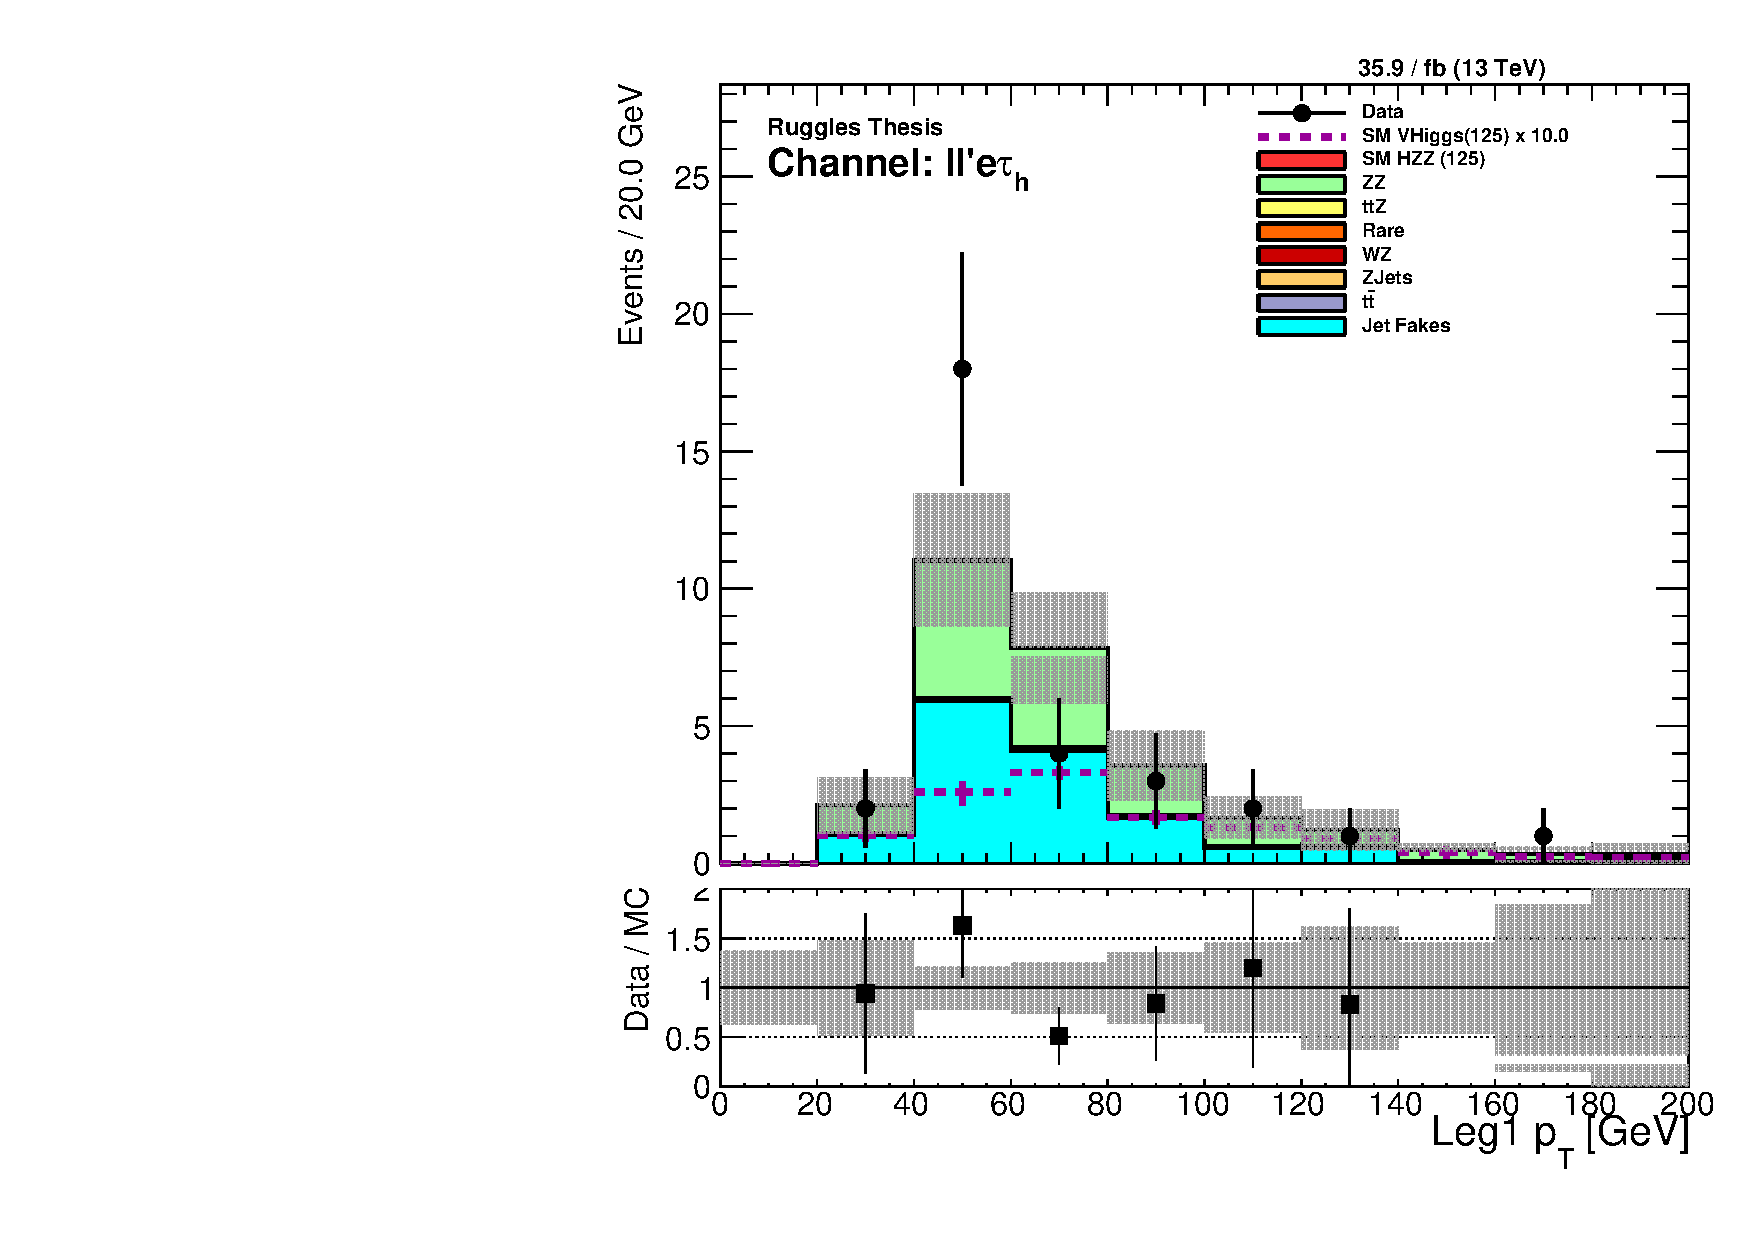
\includegraphics[width=0.49\textwidth]{higgs_to_taus_vh/plots/zh/fr_OS_control/LLET/pt_1.pdf}
     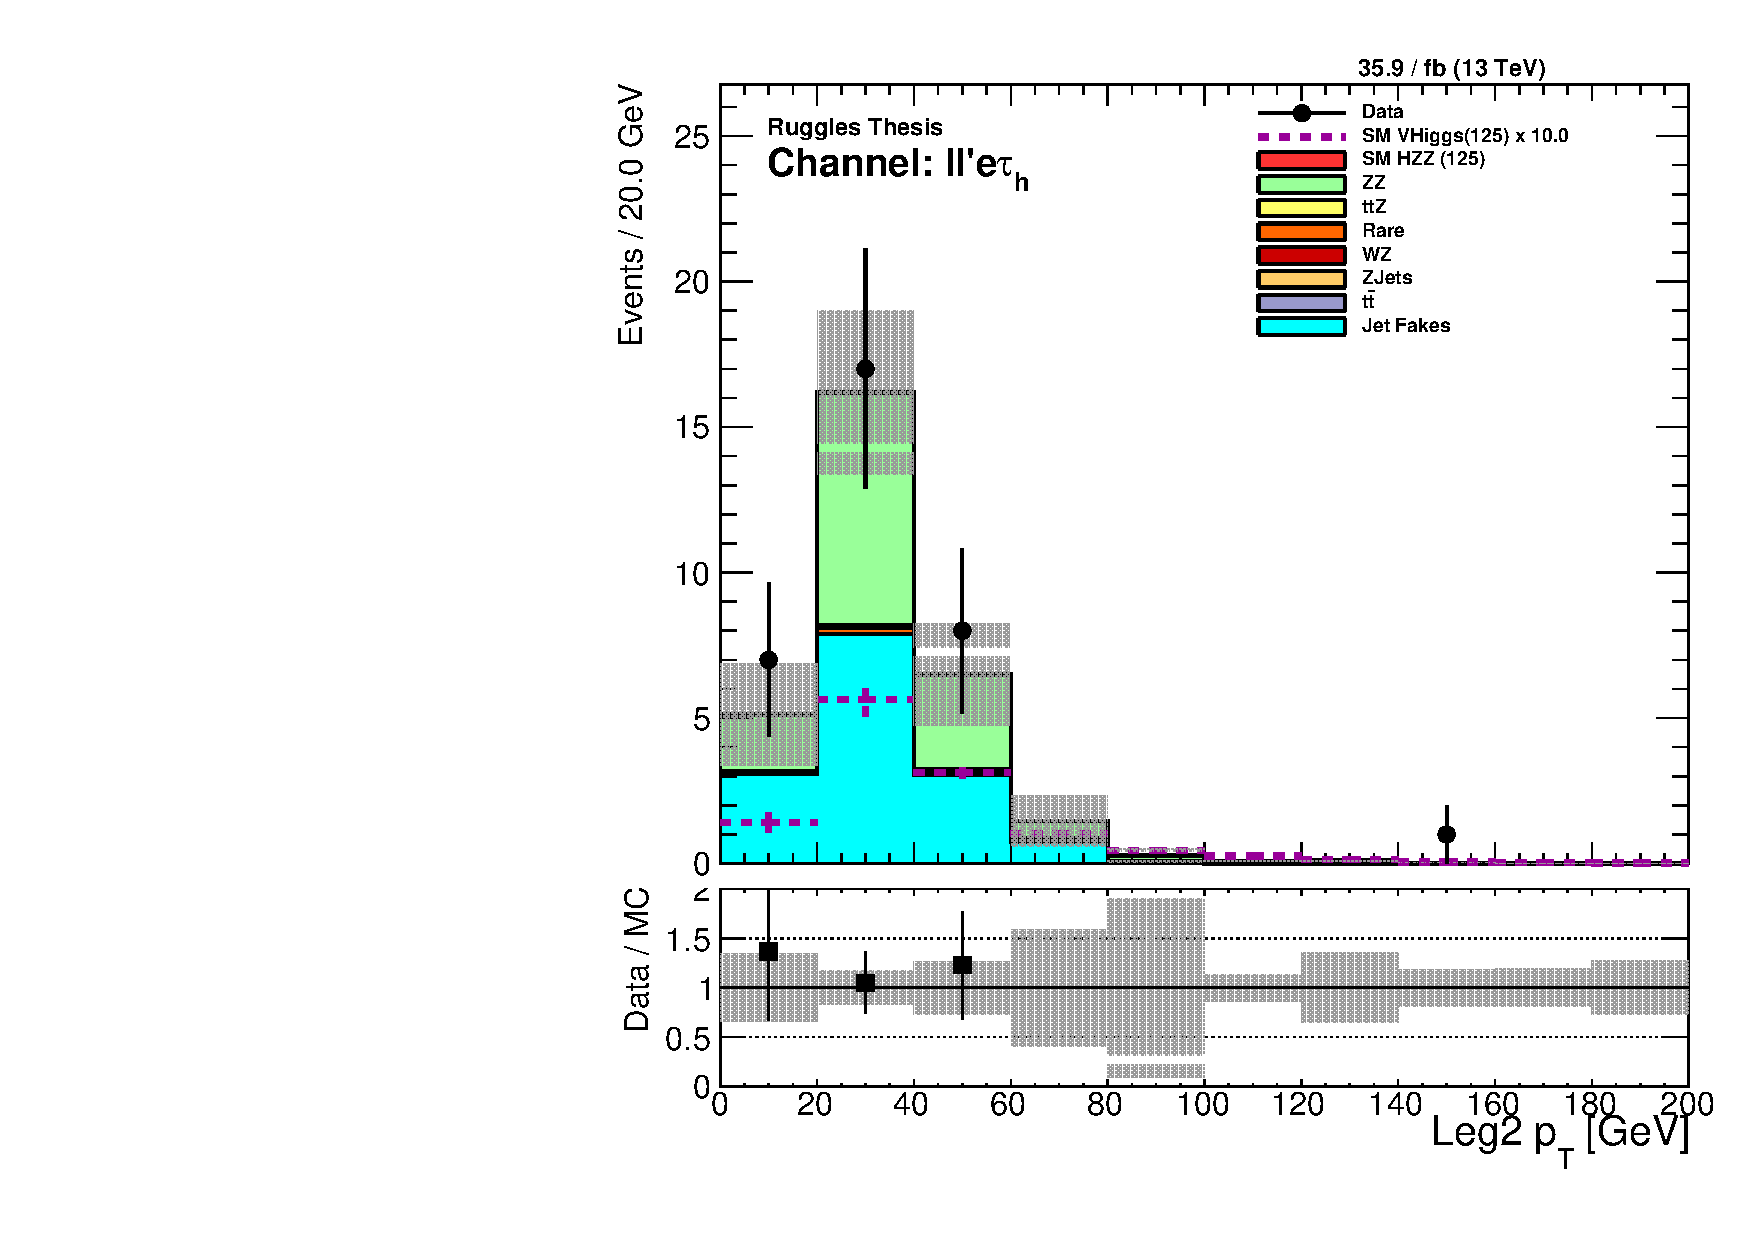
\includegraphics[width=0.49\textwidth]{higgs_to_taus_vh/plots/zh/fr_OS_control/LLET/pt_2.pdf}
     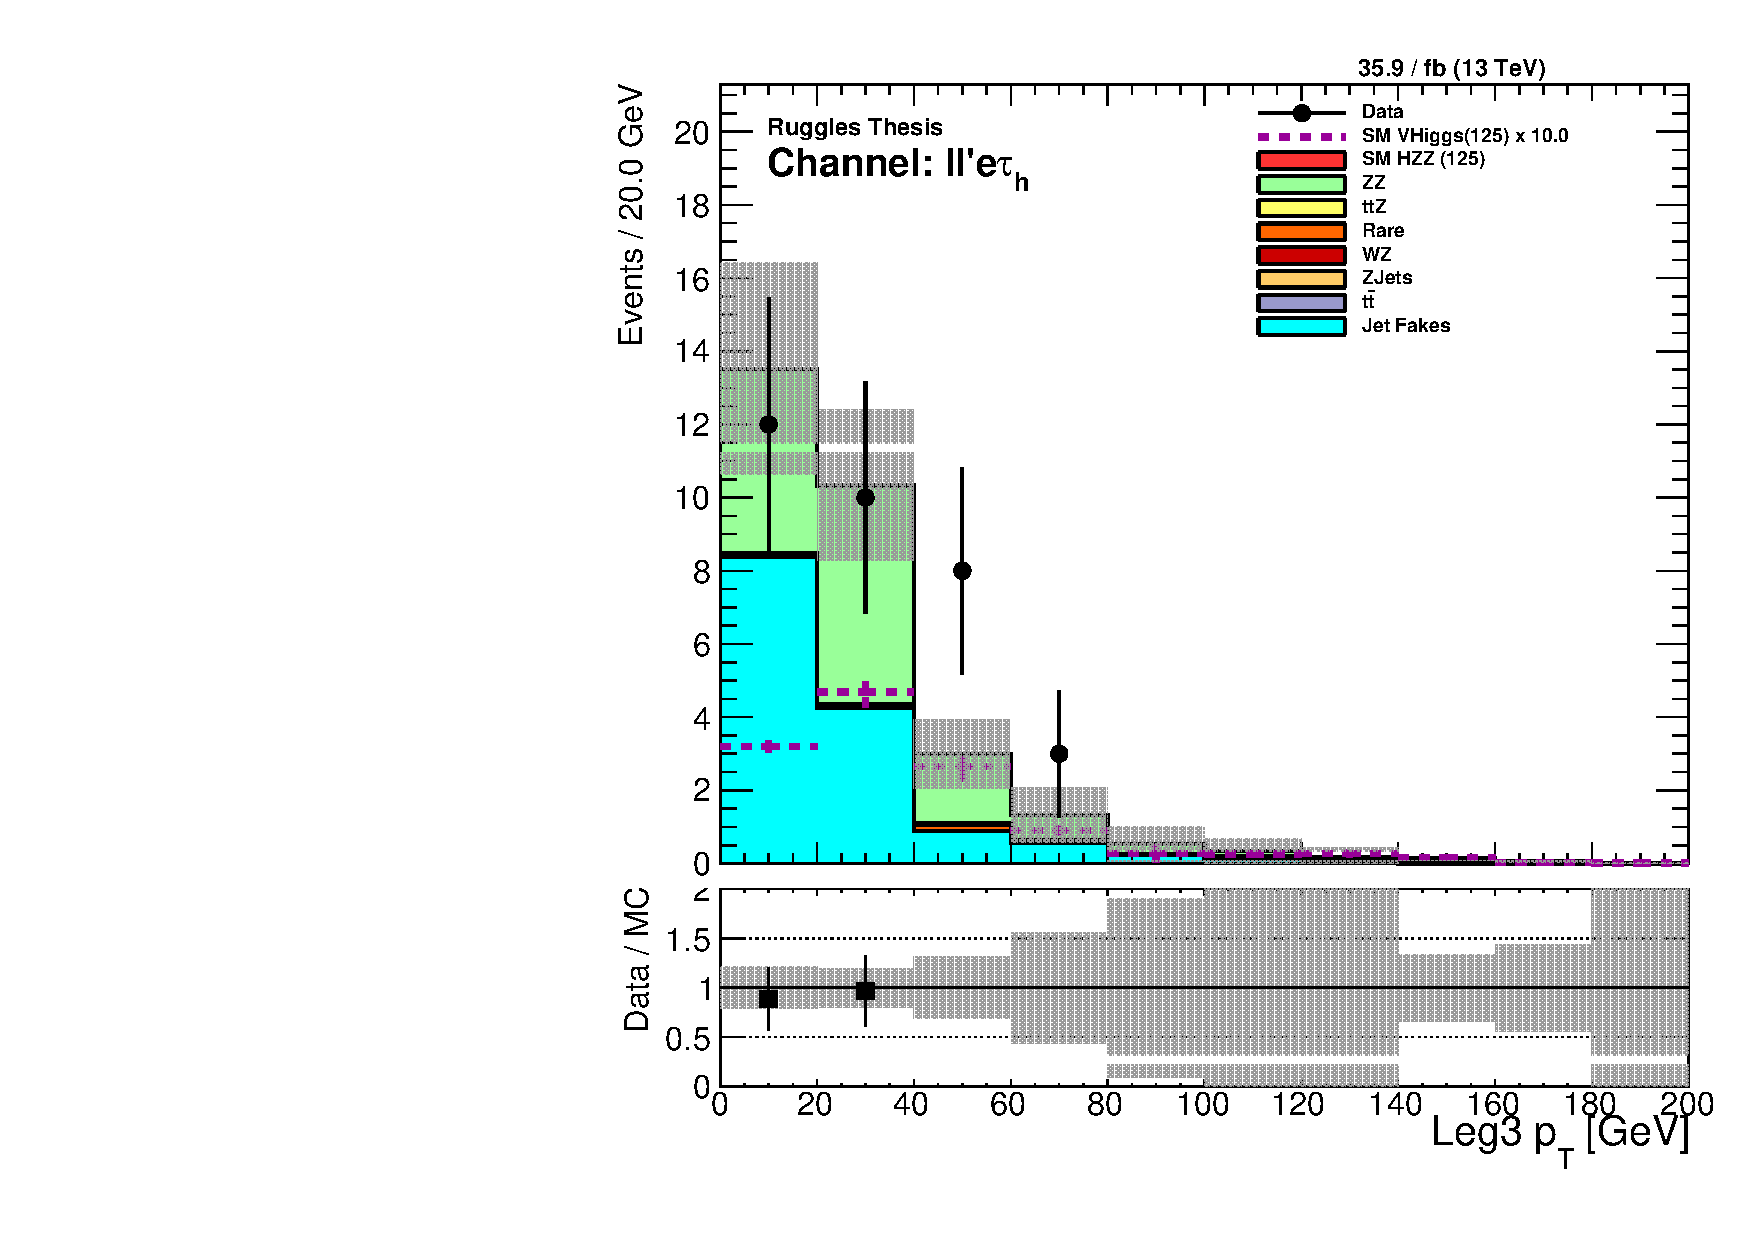
\includegraphics[width=0.49\textwidth]{higgs_to_taus_vh/plots/zh/fr_OS_control/LLET/pt_3.pdf}
     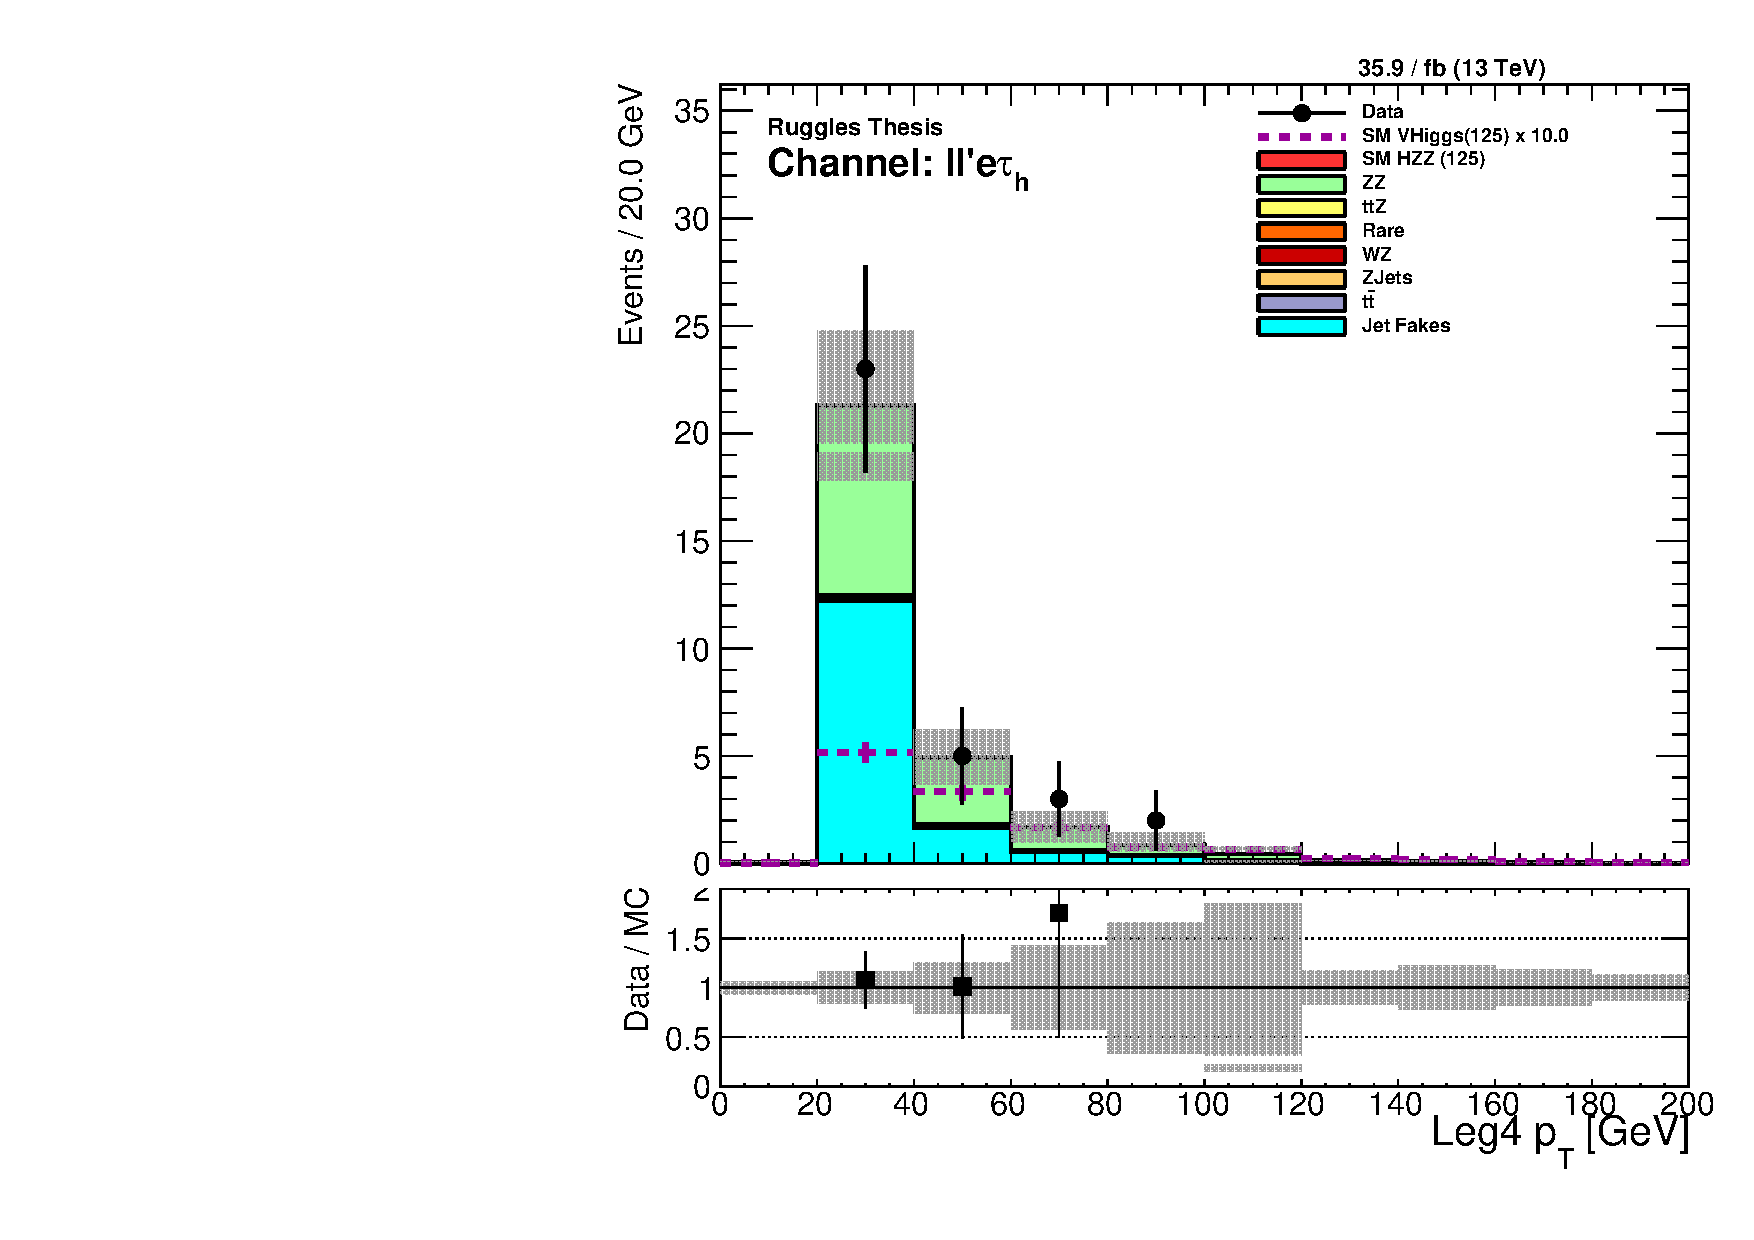
\includegraphics[width=0.49\textwidth]{higgs_to_taus_vh/plots/zh/fr_OS_control/LLET/pt_4.pdf}
     \caption{
Pre-fit $\pt$ distributions showing statistical uncertainties only for the 
four leptons in the $\ell\ell\Pe\tauh$ final states.
(top left) and (top right) leading and subleading $\ell$ from $\PZ$,
(bottom left) and (bottom right) $\Pe$ and $\tauh$ from Higgs boson candidate.
The $\PW\PH$ and $\PZ\PH$ signals are summed as $VHiggs$ and multipled by a factor of
10 times their SM expected yield.
     }
     \label{fig:llet_pts}
\end{figure*}

\begin{figure*}[htbp]
\centering
     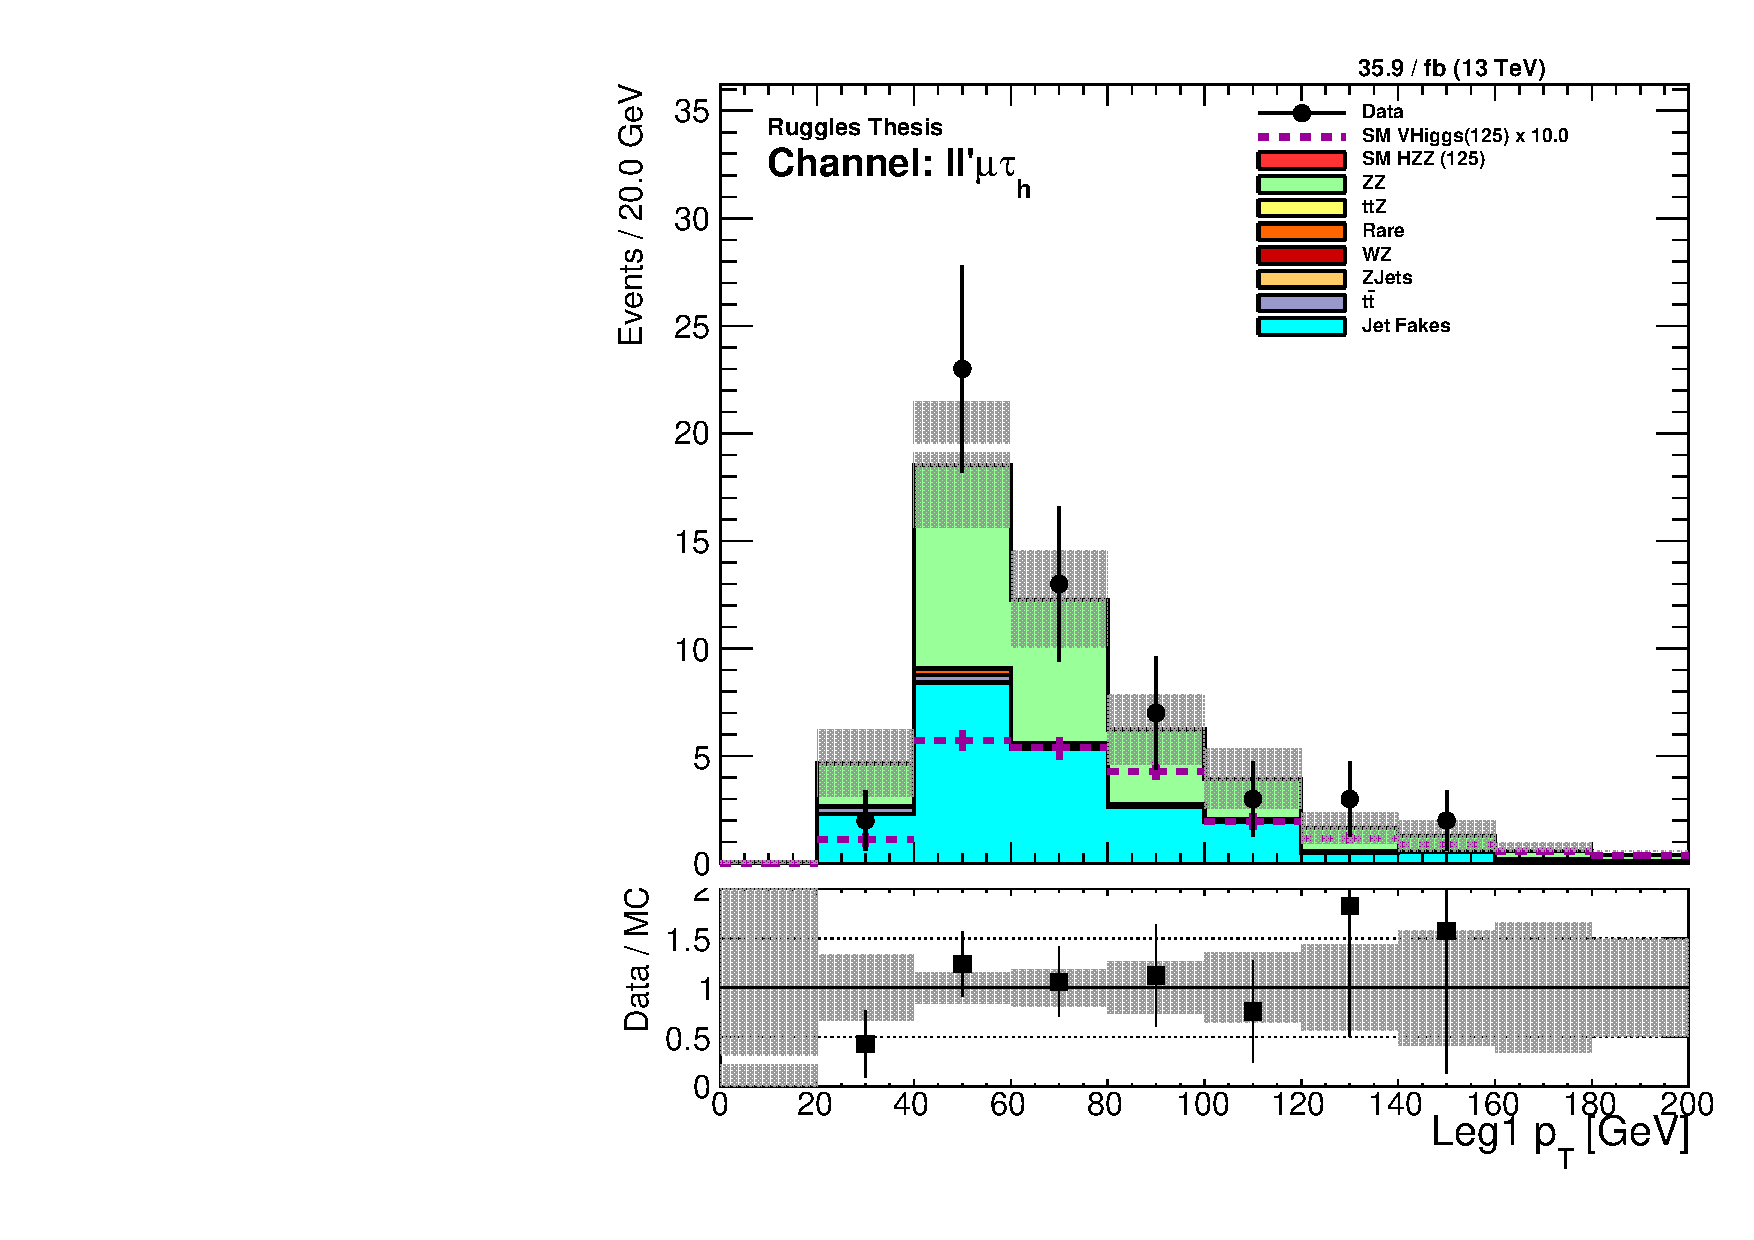
\includegraphics[width=0.49\textwidth]{higgs_to_taus_vh/plots/zh/fr_OS_control/LLMT/pt_1.pdf}
     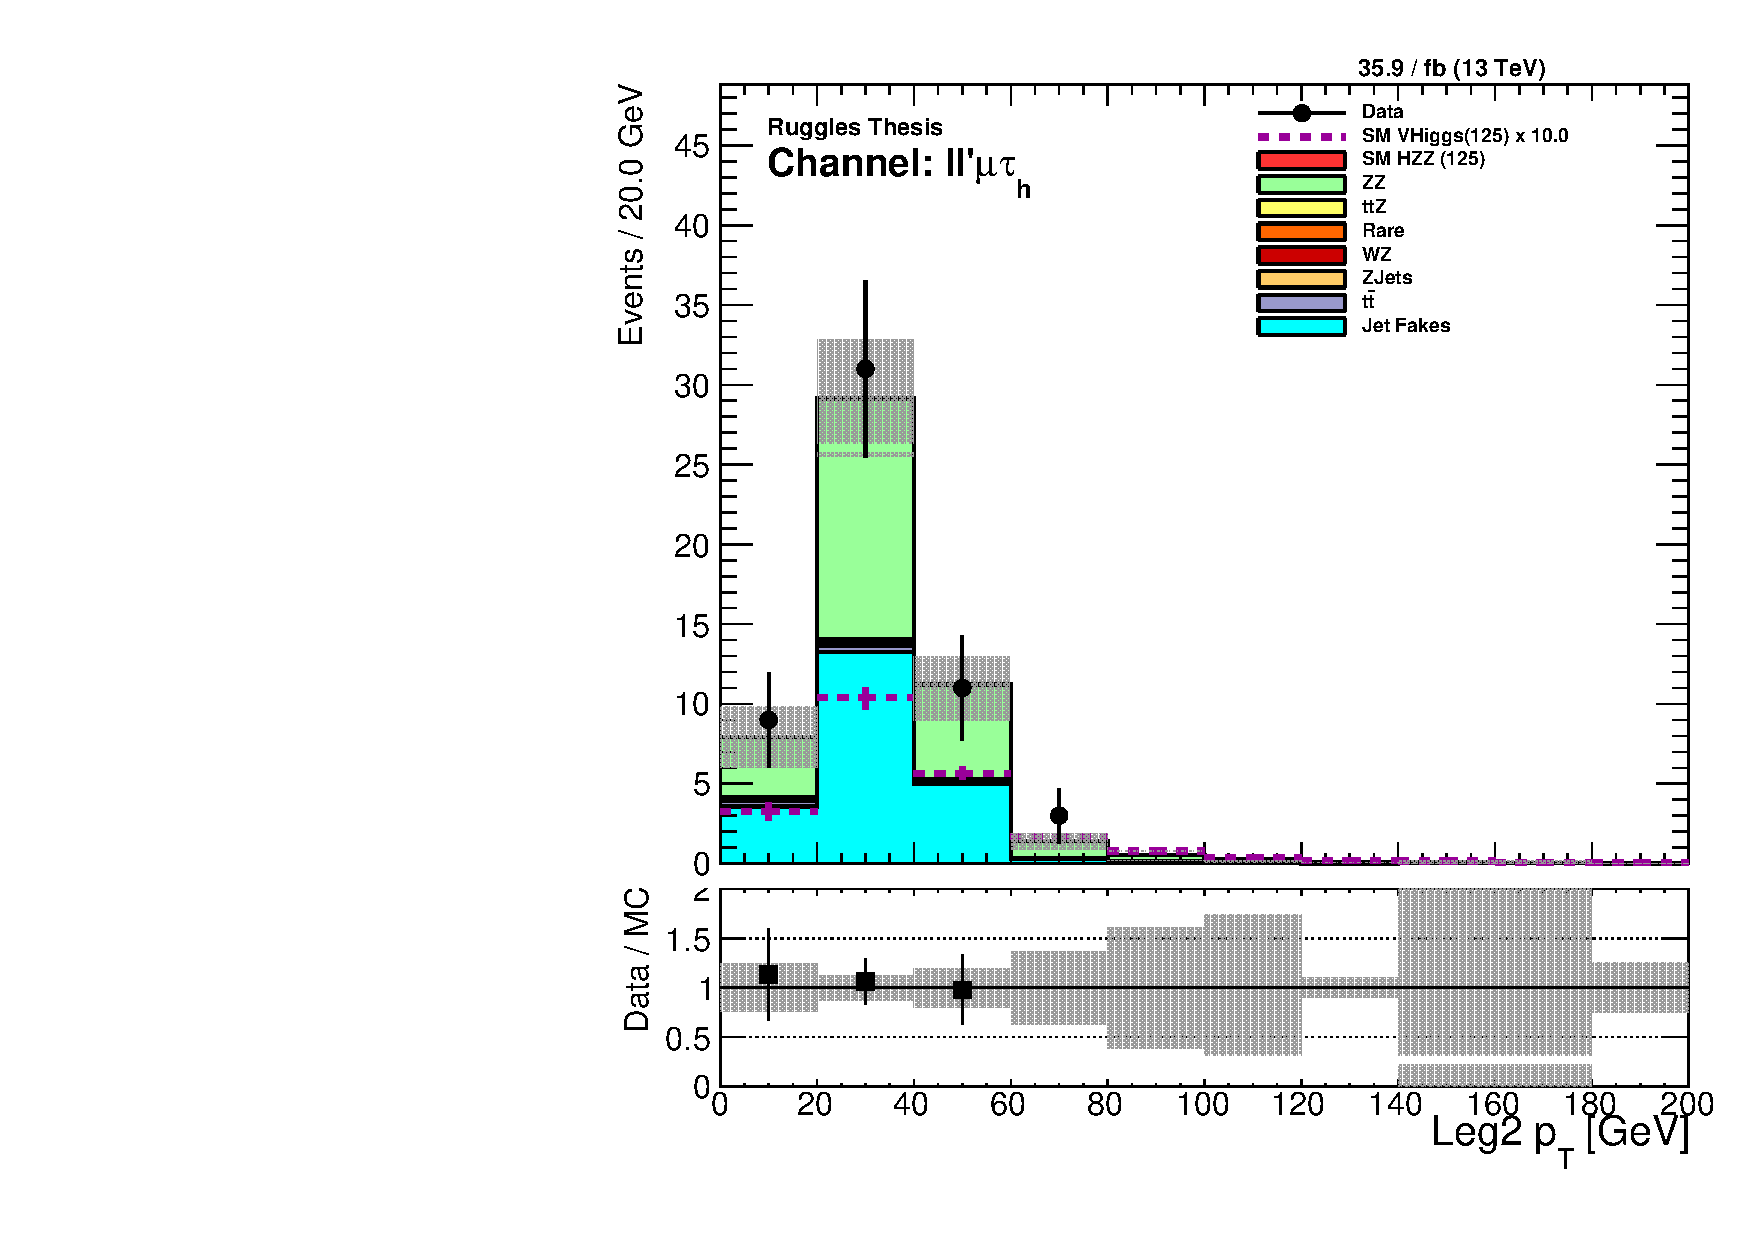
\includegraphics[width=0.49\textwidth]{higgs_to_taus_vh/plots/zh/fr_OS_control/LLMT/pt_2.pdf}
     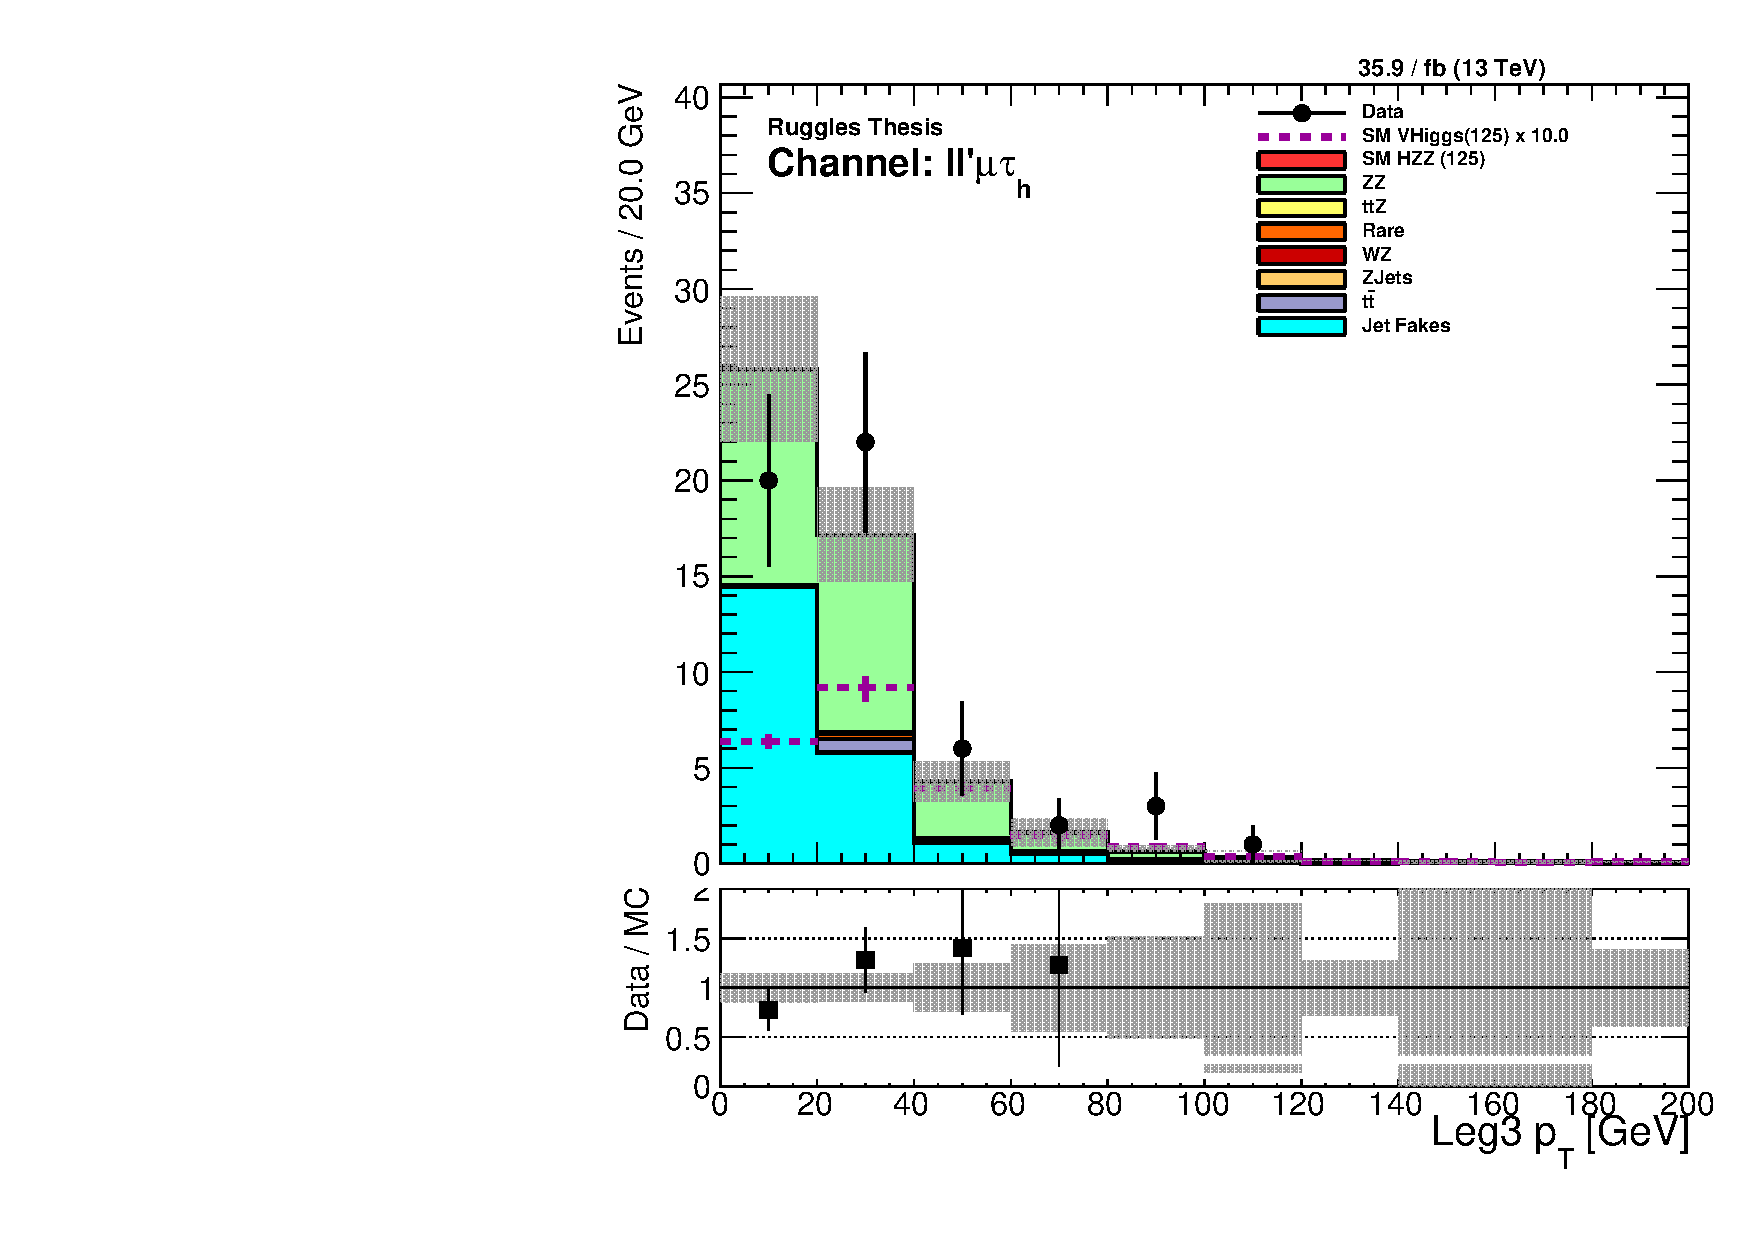
\includegraphics[width=0.49\textwidth]{higgs_to_taus_vh/plots/zh/fr_OS_control/LLMT/pt_3.pdf}
     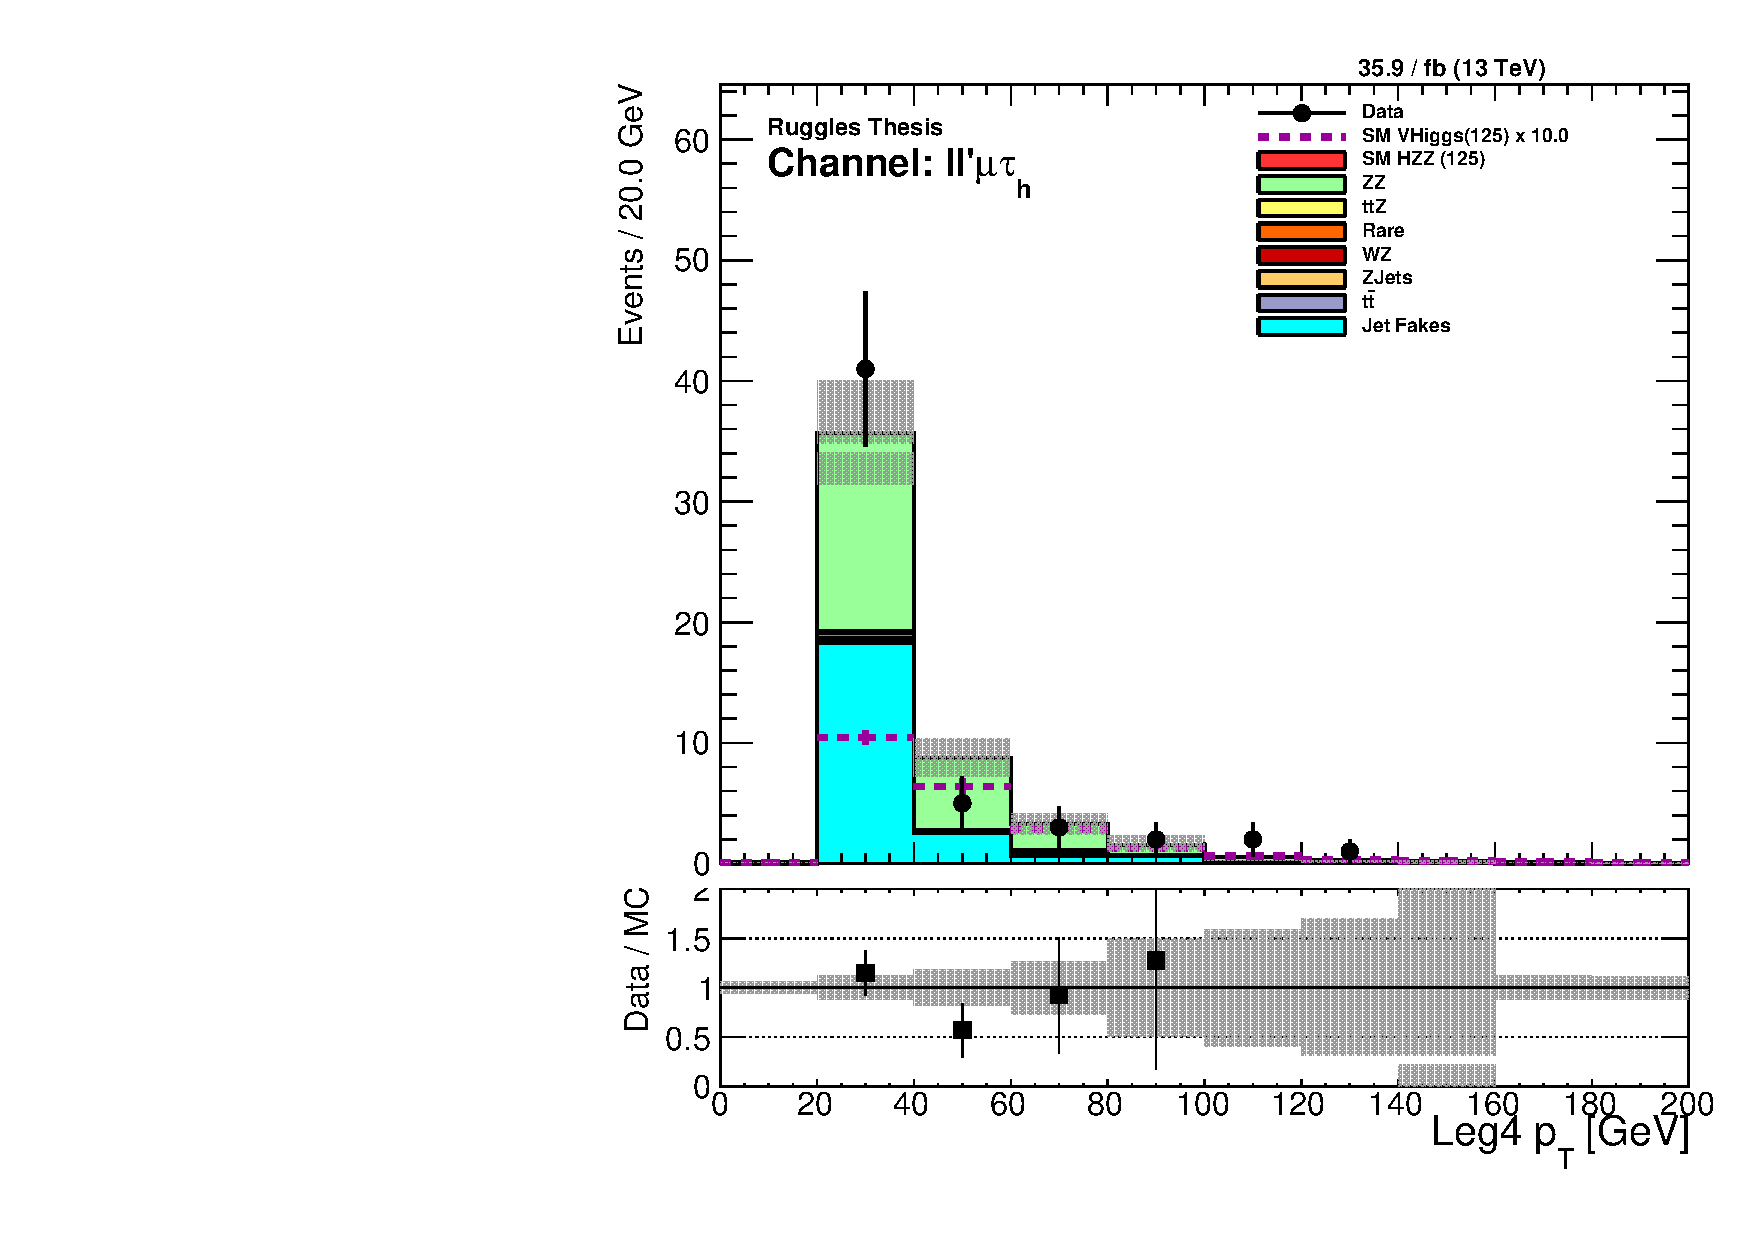
\includegraphics[width=0.49\textwidth]{higgs_to_taus_vh/plots/zh/fr_OS_control/LLMT/pt_4.pdf}
     \caption{
Pre-fit $\pt$ distributions showing statistical uncertainties only for the 
four leptons in the $\ell\ell\Pgm\tauh$ final states.
(top left) and (top right) leading and subleading $\ell$ from $\PZ$,
(bottom left) and (bottom right) $\Pgm$ and $\tauh$ from Higgs boson candidate.
The $\PW\PH$ and $\PZ\PH$ signals are summed as $VHiggs$ and multipled by a factor of
10 times their SM expected yield.
     }
     \label{fig:llmt_pts}
\end{figure*}

\begin{figure*}[htbp]
\centering
     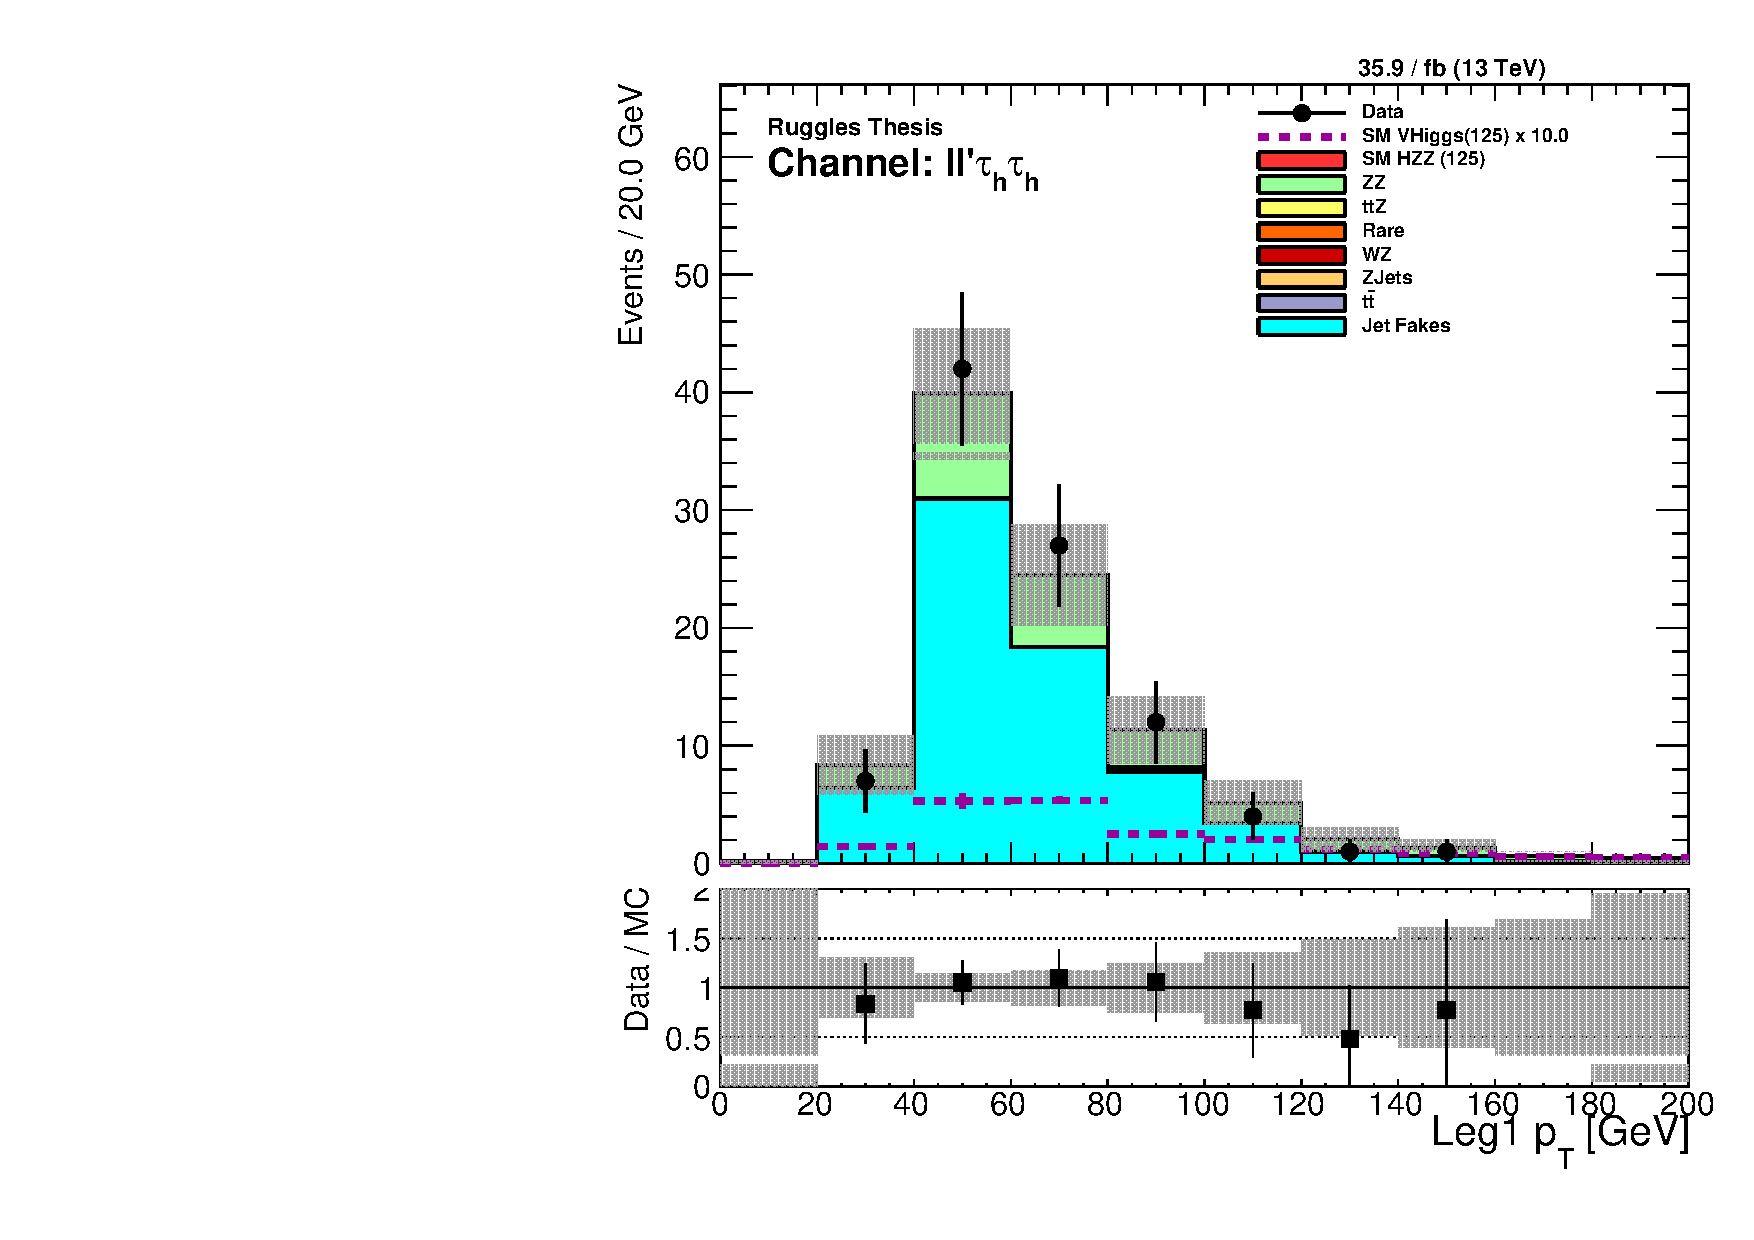
\includegraphics[width=0.49\textwidth]{higgs_to_taus_vh/plots/zh/fr_OS_control/LLTT/pt_1.pdf}
     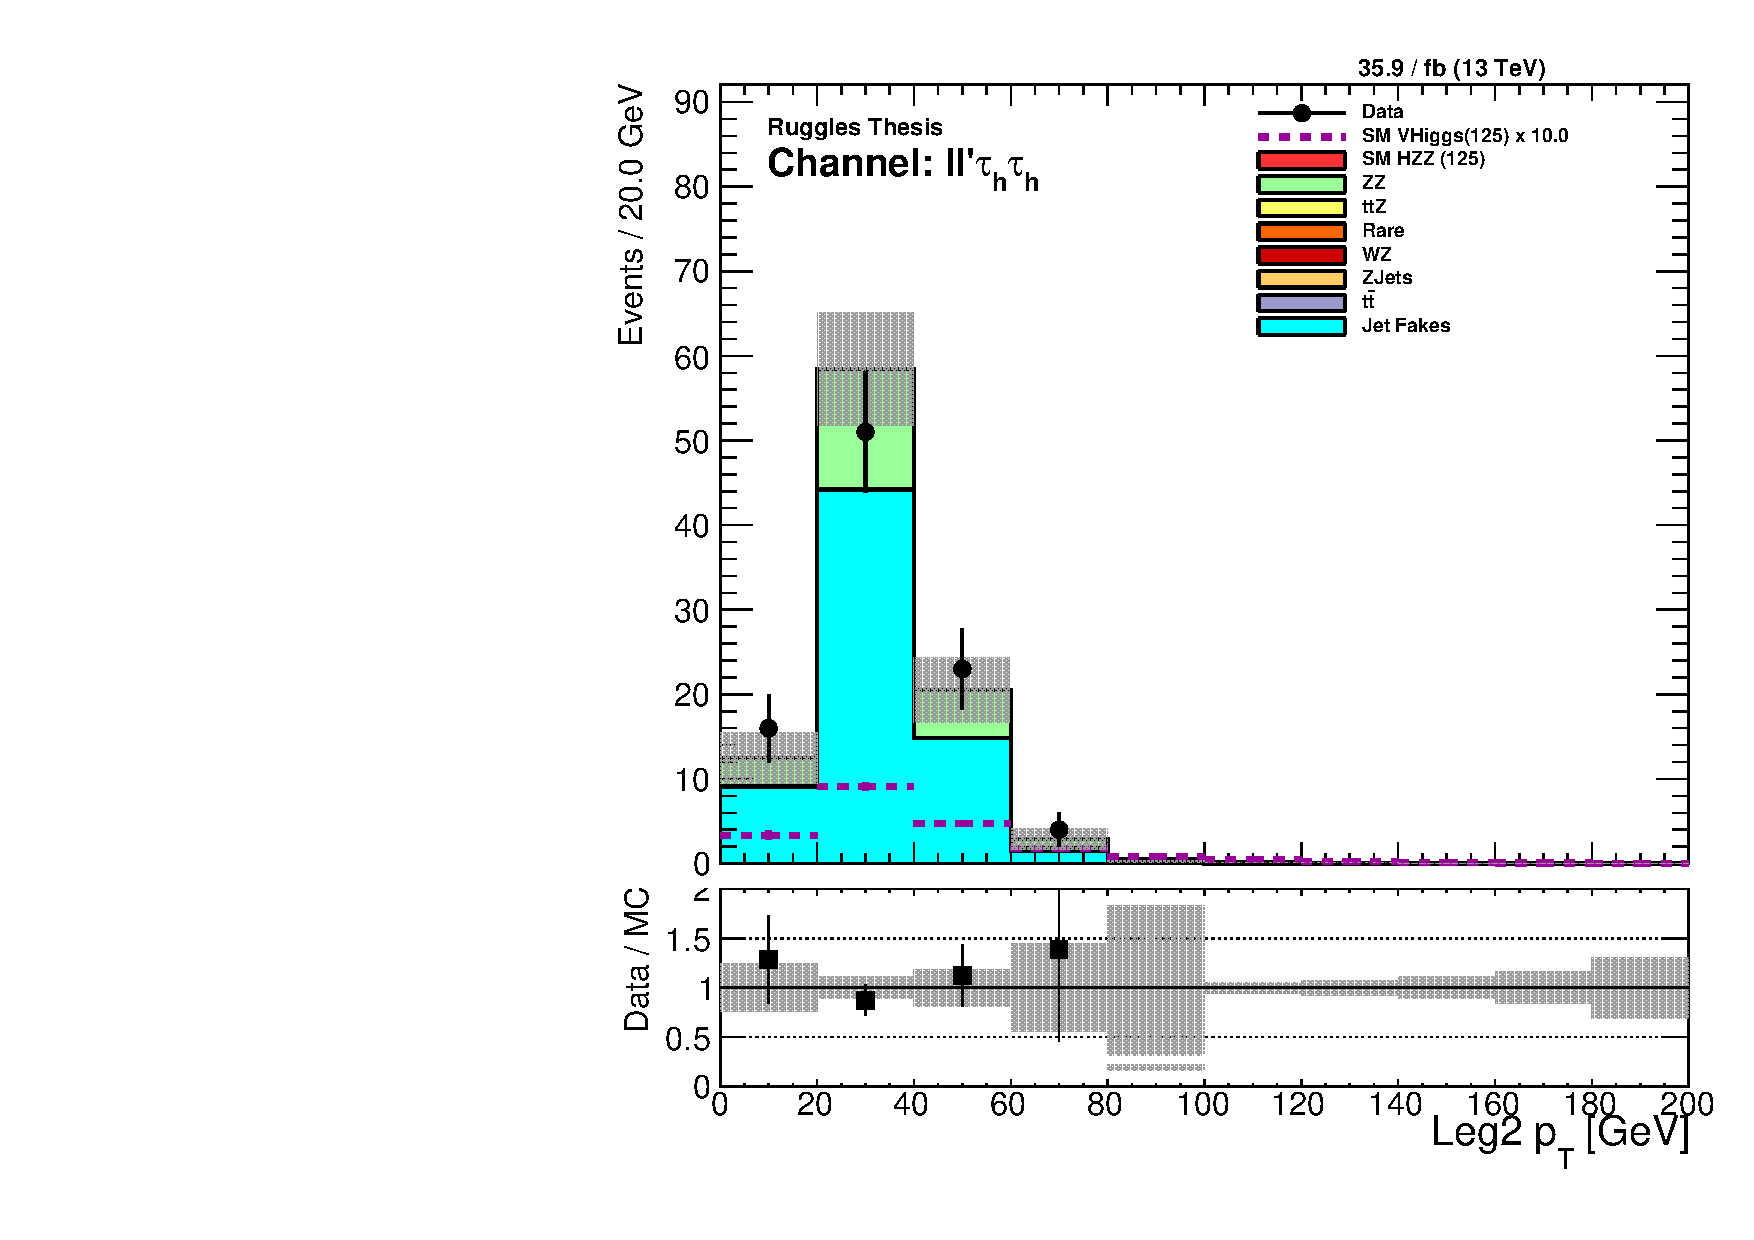
\includegraphics[width=0.49\textwidth]{higgs_to_taus_vh/plots/zh/fr_OS_control/LLTT/pt_2.pdf}
     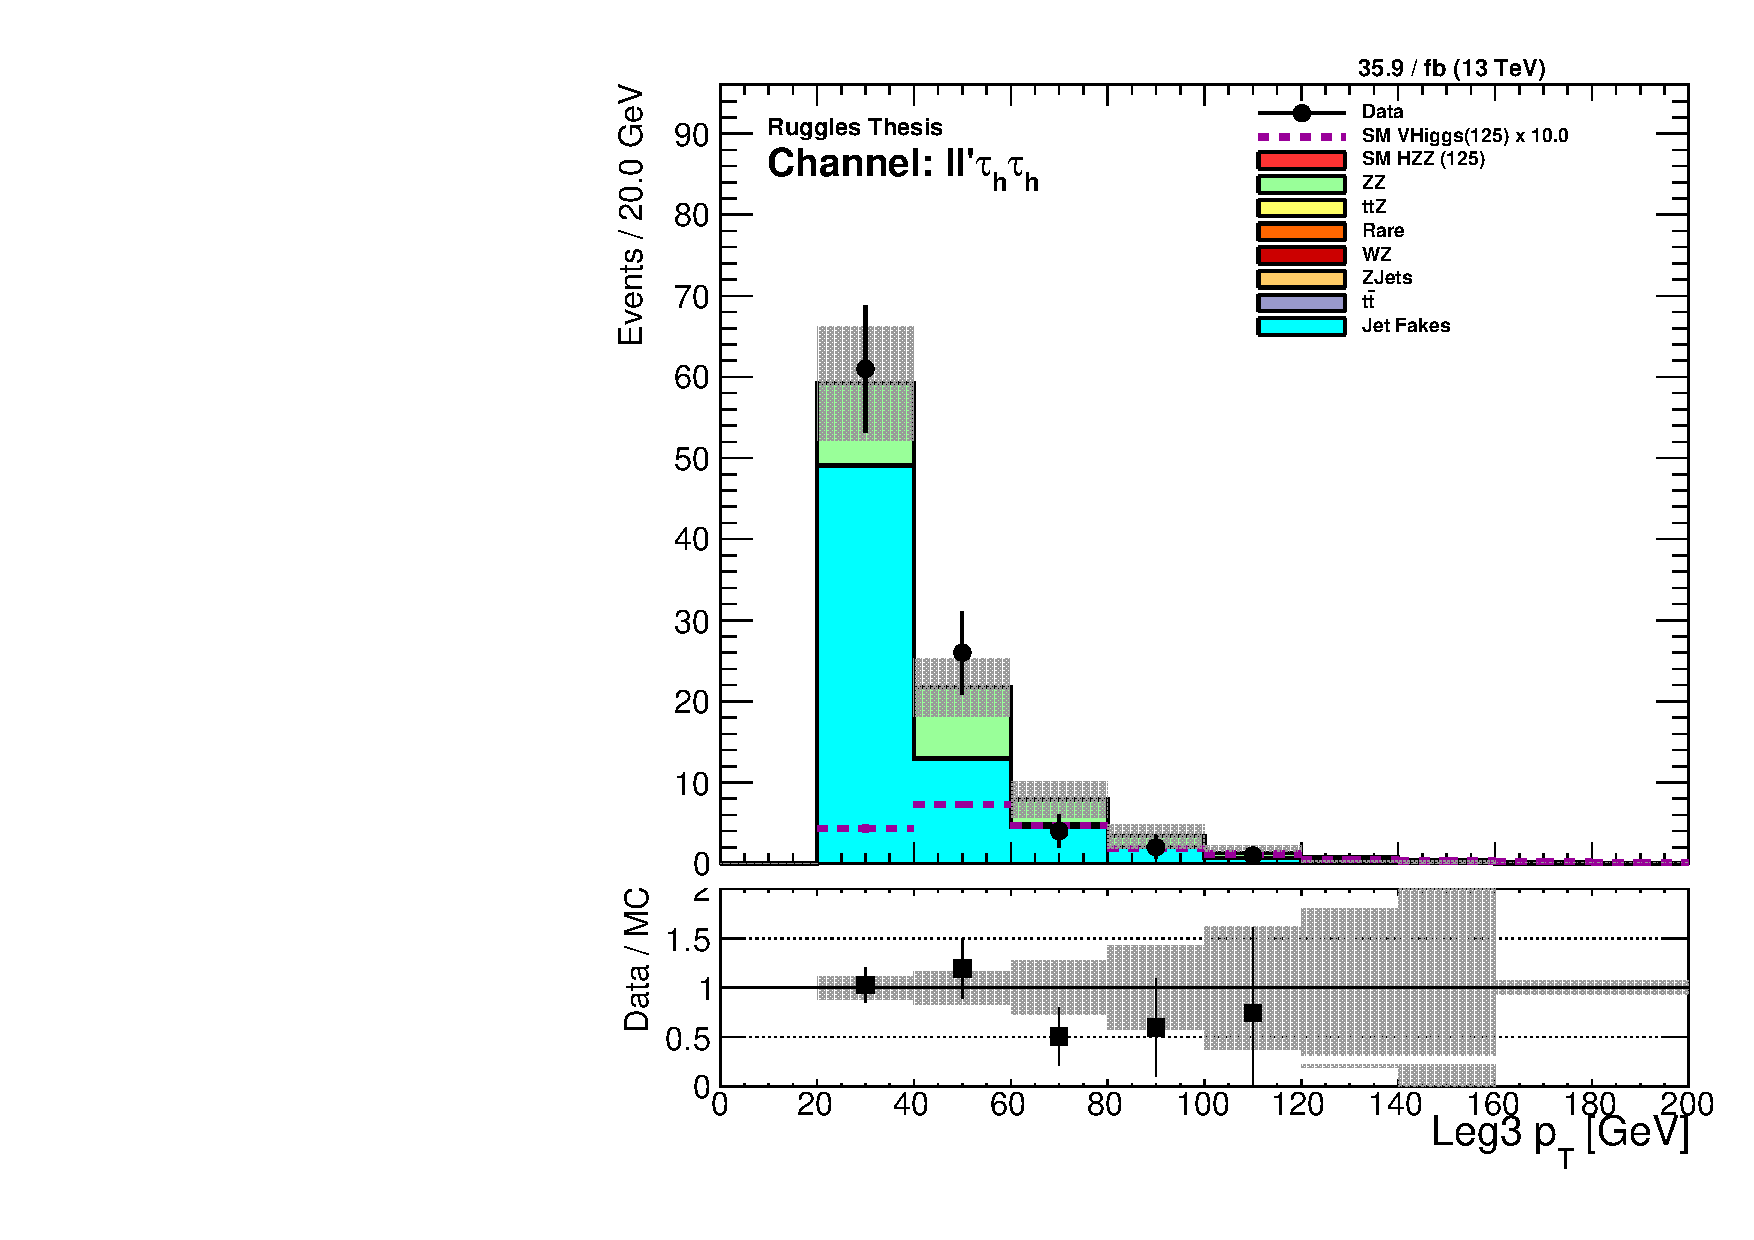
\includegraphics[width=0.49\textwidth]{higgs_to_taus_vh/plots/zh/fr_OS_control/LLTT/pt_3.pdf}
     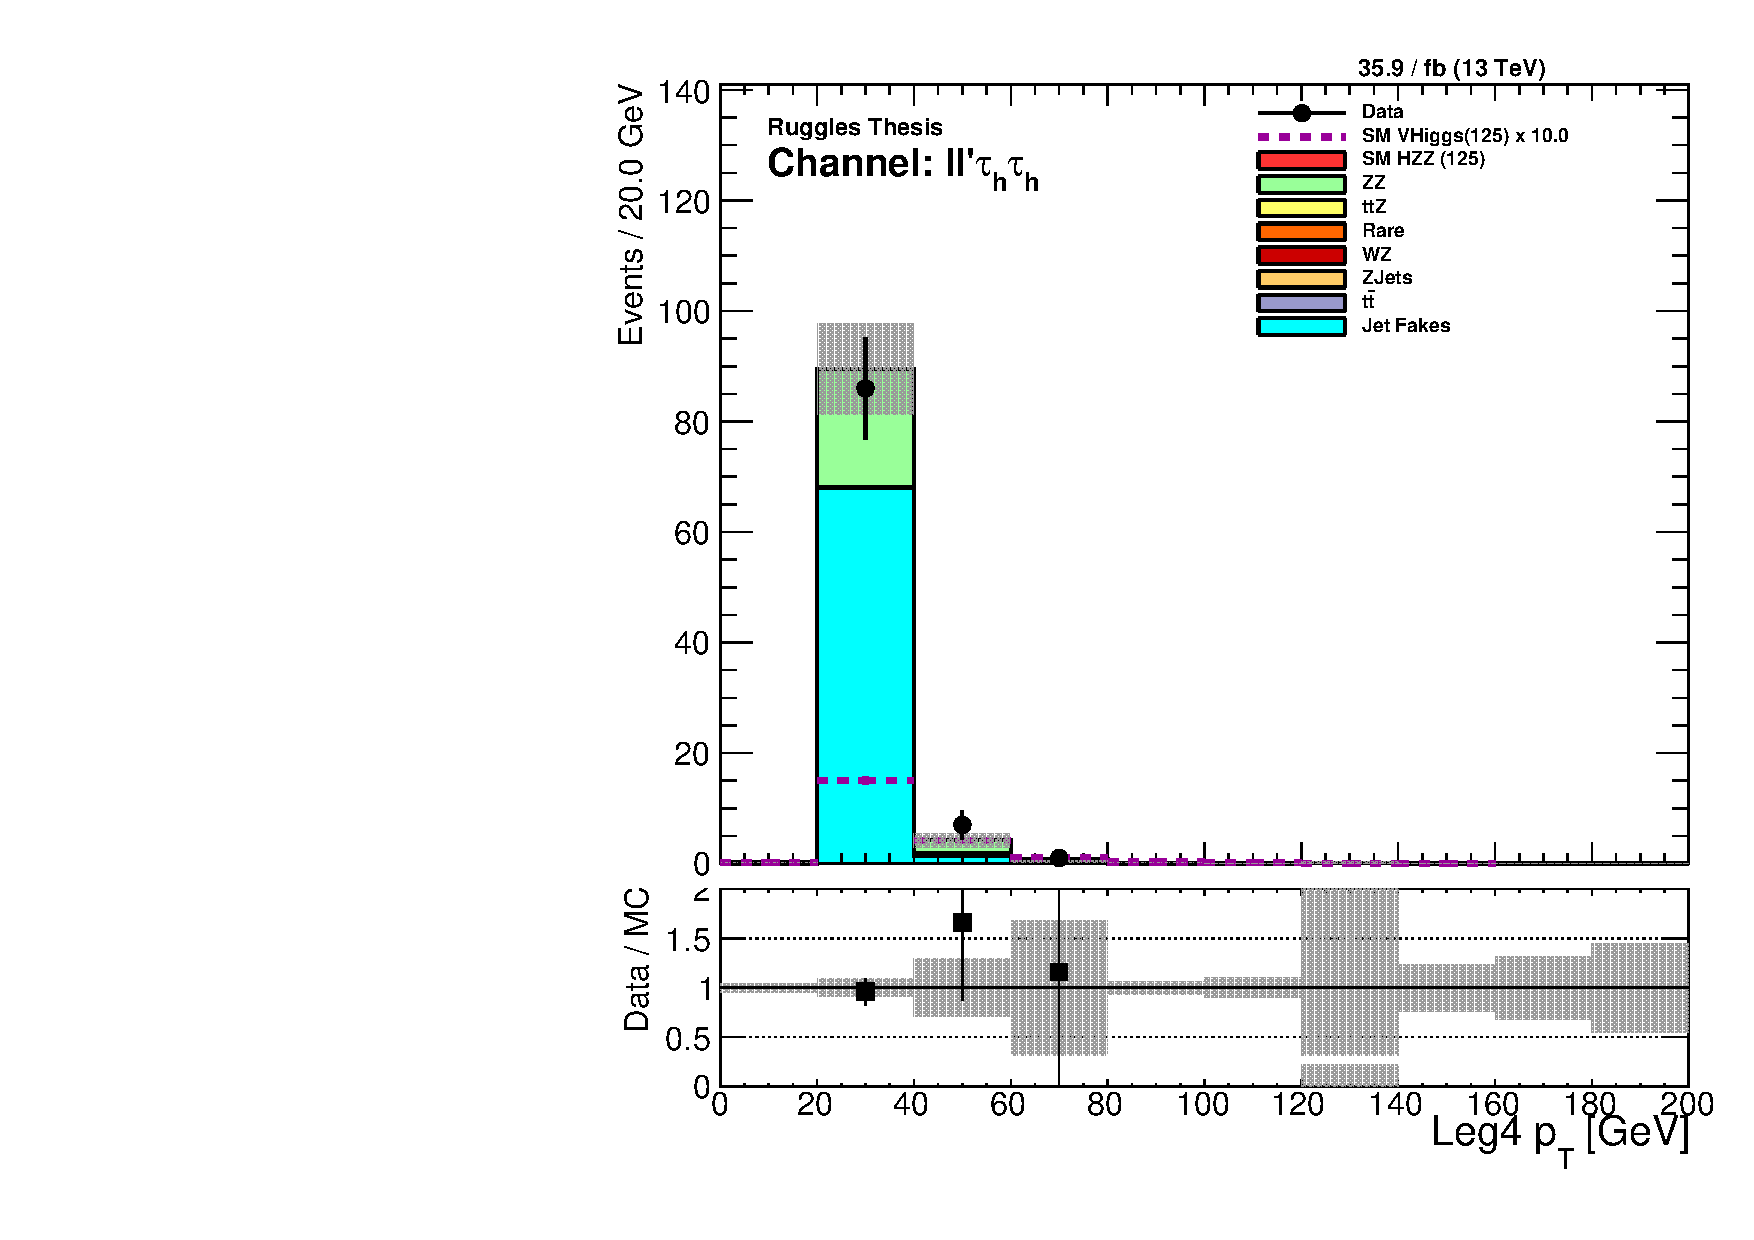
\includegraphics[width=0.49\textwidth]{higgs_to_taus_vh/plots/zh/fr_OS_control/LLTT/pt_4.pdf}
     \caption{
Pre-fit $\pt$ distributions showing statistical uncertainties only for the 
four leptons in the $\ell\ell\tauh\tauh$ final states.
(top left) and (top right) leading and subleading $\ell$ from $\PZ$,
(bottom left) and (bottom right) leading and subleading $\tauh$ from Higgs boson candidate.
The $\PW\PH$ and $\PZ\PH$ signals are summed as $VHiggs$ and multipled by a factor of
10 times their SM expected yield.
     }
     \label{fig:lltt_pts}
\end{figure*}

\begin{figure*}[htbp]
\centering
     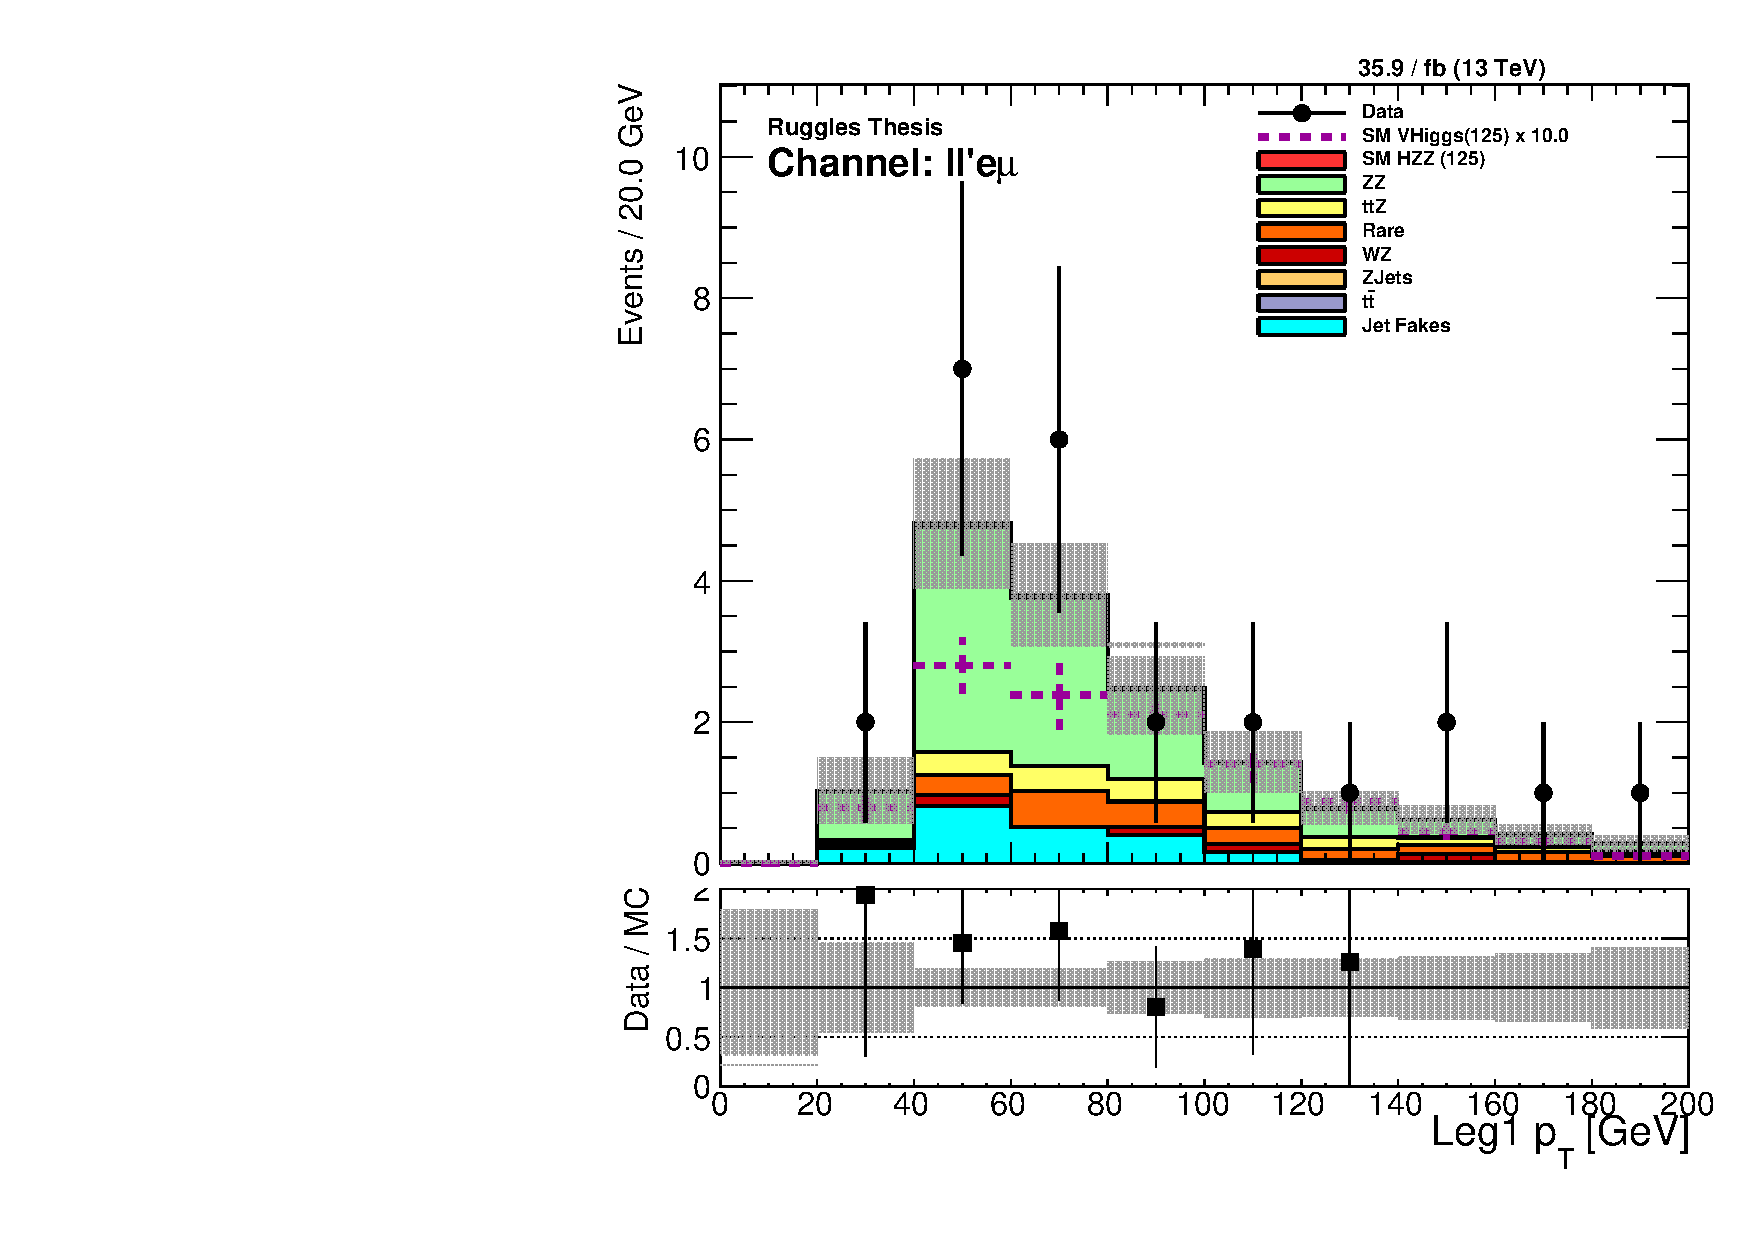
\includegraphics[width=0.49\textwidth]{higgs_to_taus_vh/plots/zh/fr_OS_control/LLEM/pt_1.pdf}
     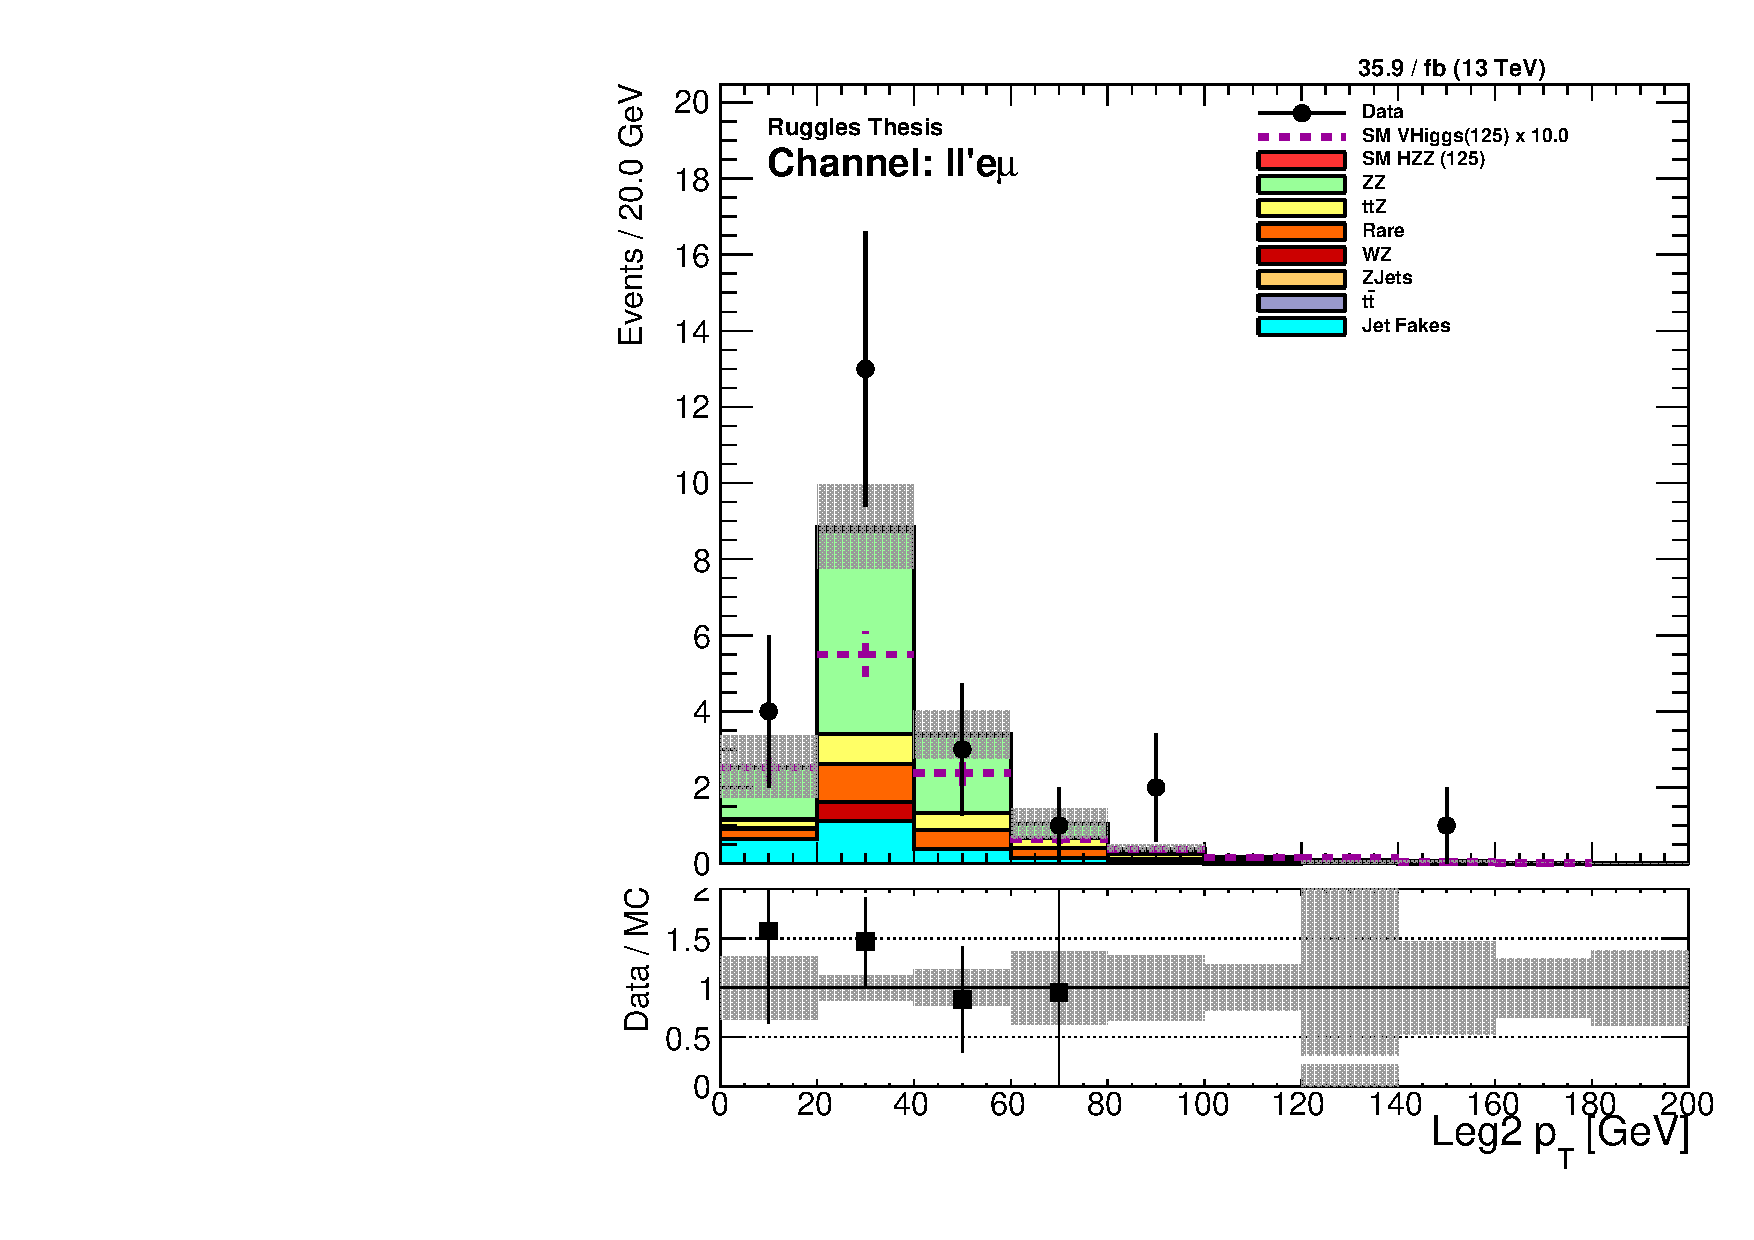
\includegraphics[width=0.49\textwidth]{higgs_to_taus_vh/plots/zh/fr_OS_control/LLEM/pt_2.pdf}
     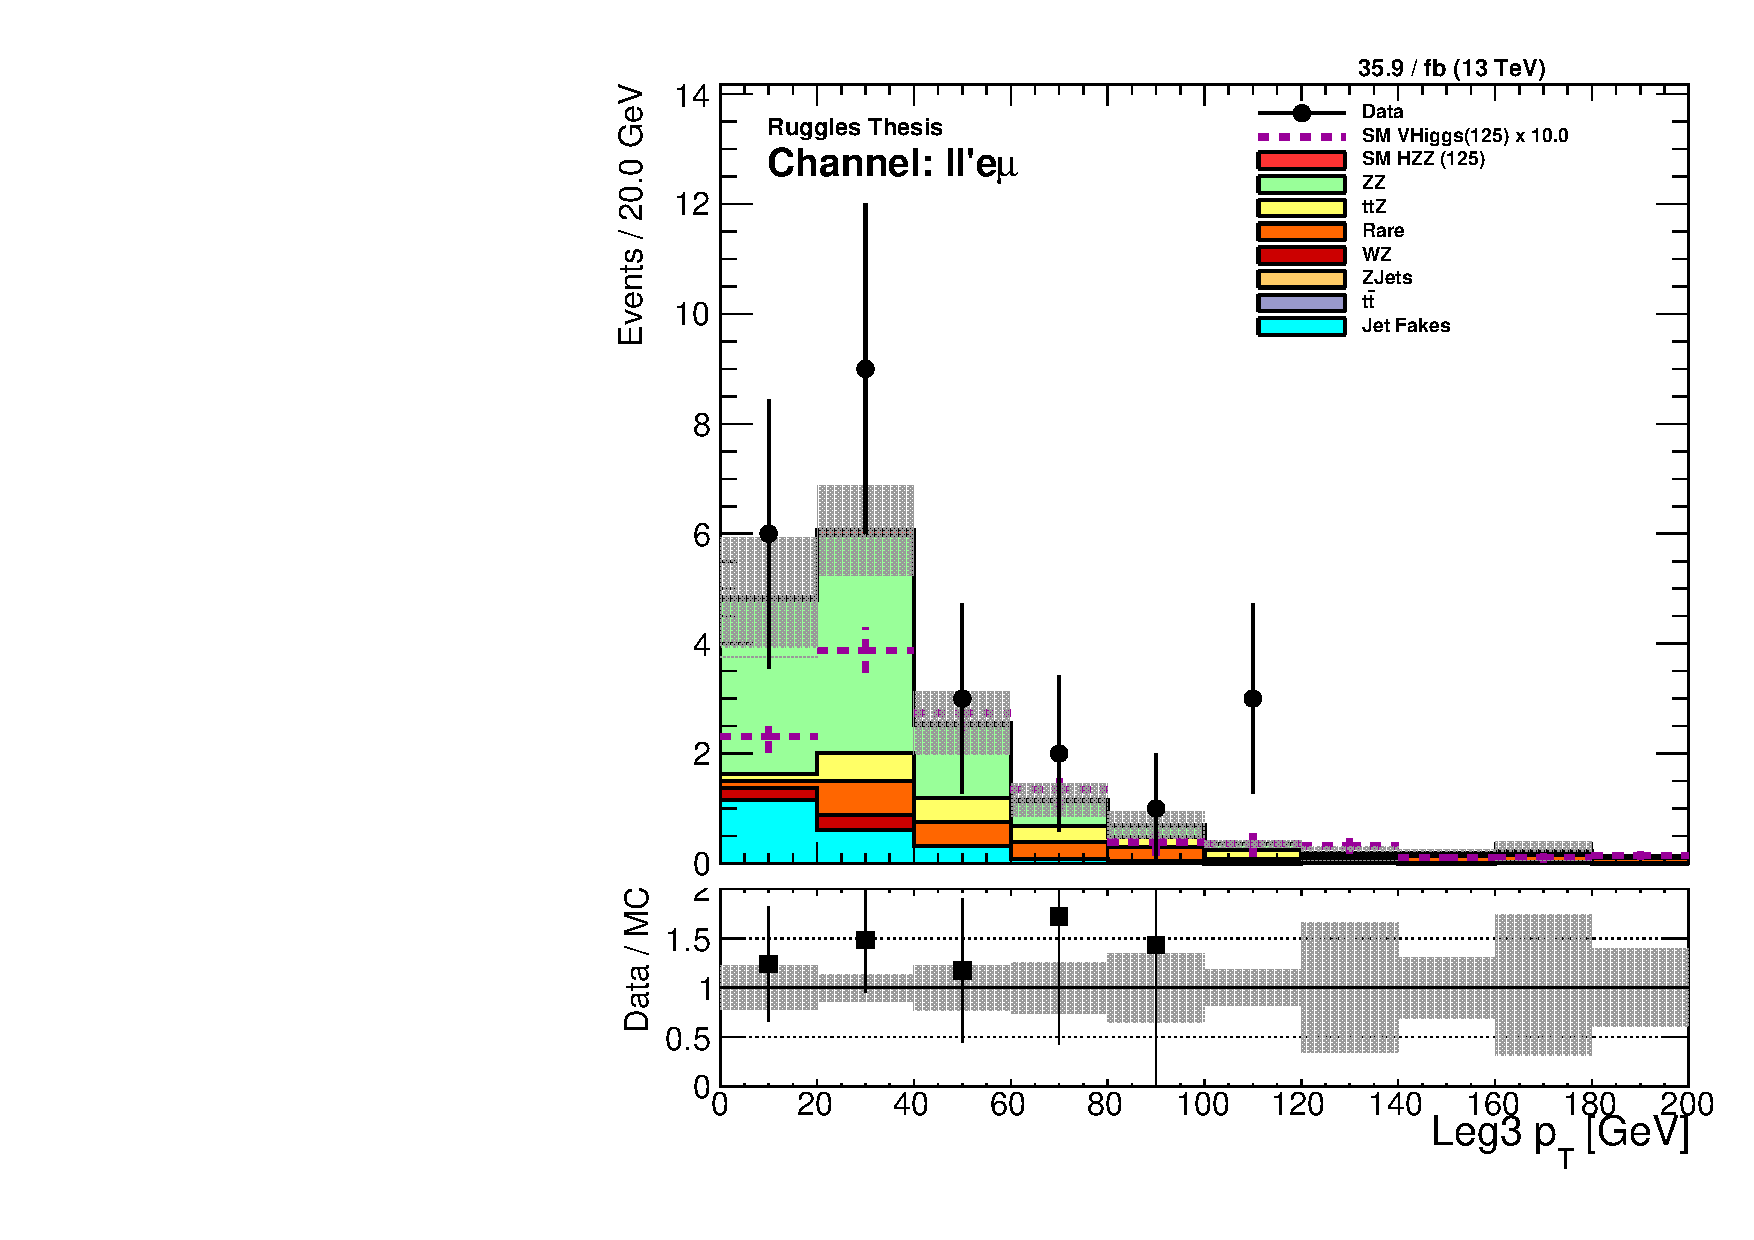
\includegraphics[width=0.49\textwidth]{higgs_to_taus_vh/plots/zh/fr_OS_control/LLEM/pt_3.pdf}
     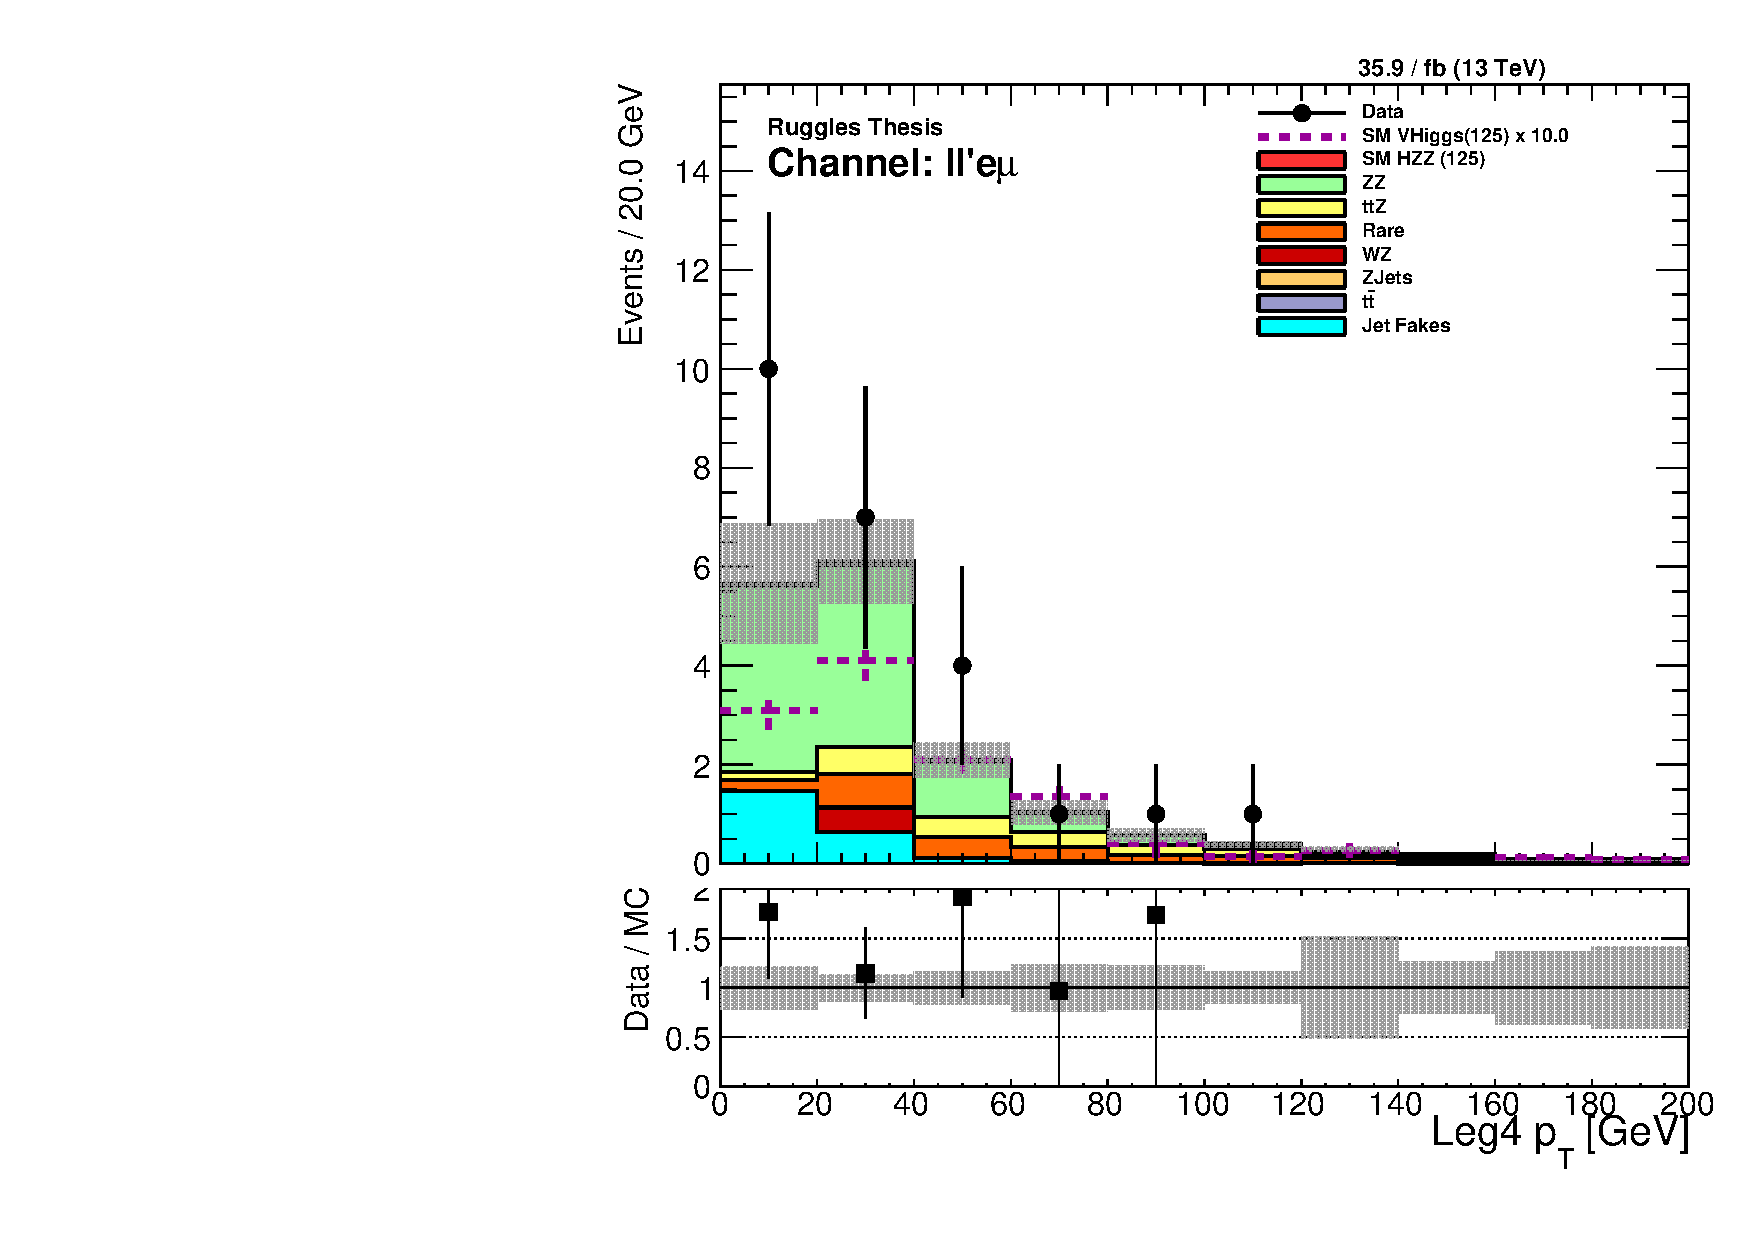
\includegraphics[width=0.49\textwidth]{higgs_to_taus_vh/plots/zh/fr_OS_control/LLEM/pt_4.pdf}
     \caption{
Pre-fit $\pt$ distributions showing statistical uncertainties only for the 
four leptons in the $\ell\ell\Pe\Pgm$ final states.
(top left) and (top right) leading and subleading $\ell$ from $\PZ$,
(bottom left) and (bottom right) $\Pe$ and $\Pgm$ from Higgs boson candidate.
The $\PW\PH$ and $\PZ\PH$ signals are summed as $VHiggs$ and multipled by a factor of
10 times their SM expected yield.
     }
     \label{fig:llem_pts}
\end{figure*}



\section{Monte Carlo Corrections}
\label{sec:vh_mc_corrections}
Corrections are applied to the simulated Monte Carlo samples to help correct for measured differences
between observed data and expectations based on simulation. Many of these corrections are designed
to correct differences in reconstruction and identification efficiencies for leptons between data
and simulation. These corrections are derived in
fully orthogonal regions from the associated production analysis signal regions.
The Monte Carlo corrections applied in the associated production analysis are identical to those
applied in the $ggH$ and VBF targeted analysis when applicable, see 
Section~\ref{sec:mc_corrections} for details.



\section{Systematic Uncertainties}
\label{sec:vh_systematics}
The systematic uncertainty model used for the associated production analysis share many
similarities with the uncertainty model used for the $ggH$ and VBF targeted analysis
considering the many shared object definitions, simulated backgrounds, and simulated $\htt$
signal samples.
Specific nuisances with identical treatment are:
\begin{itemize}
\item Uncertainty of the $\tauh$ identification efficiency for genuine $\tauh$
\item Uncertainty on the visible energy scale of genuine $\tauh$ leptons
\item Uncertainties in the muon and electron identification, isolation, and trigger efficiencies
\item Uncertainty related to discarding events with a b-tagged jet
\item \etvecmiss scale uncertainties; these uncertainties are skipped for the
$\PW\PH$ semileptonic final states where \etvecmiss is not used
\item Uncertainty on the finite number of simulated events
\item Uncertainty in the integrated luminosity
\end{itemize}
The full details of how these identical nuisances are treated can be found in
Section~\ref{sec:htt_systematics}.


\subsection{Simulated Background Estimation Uncertainties}
Uncertainties from the renormalization and the factorization scales, and from the 
choice of the PDF set (Section~\ref{sec:sim_pdf}), are taken into account for the $\PZ\PZ$ and $\PW\PZ$ 
background processes. The uncertainty from the renormalization and factorization 
scales is determined by varying these scales between 0.5 and 2 times their nominal 
value and computing the change in acceptance. This leads to yield uncertainties 
of $^{+3.2\%}_{-4.2\%}$ for the $\Pq\Pq\rightarrow \PZ\PZ$ background, and $\pm 3.2\%$ 
for the $\PW\PZ$ process. The uncertainty from the PDF set is determined following 
the PDF4LHC recommendations~\cite{Butterworth:2015oua}, and leads to yield uncertainties of $^{+3.1\%}_{-4.2\%}$ for 
the $\Pq\Pq\rightarrow \PZ\PZ$ background, and $\pm 4.5\%$ for the $\PW\PZ$ process. 
In addition, a 10\% uncertainty in the k-factor used for the $\Pg\Pg \rightarrow 
\PZ\PZ$ prediction is considered. The uncertainty in the cross section of the 
rare $\ttbar\PW$ and $\ttbar\PZ$ processes amounts to 25\%.

\subsection{Reducible Background Estimation Uncertainties}
The reducible backgrounds are estimated using the measured rates for jets to be 
misidentified as electrons, muons, or $\tauh$ discussed in 
Section~\ref{sec:vh_background_estimation}. The misidentification rates are 
measured in different bins of lepton $\pt$, and are further split between 
reconstructed decay modes for the $\tauh$. In the $\PW\PH$ final states where
the shape of the reducible background is estimated using the misidentification rate
method, the statistical uncertainty in every 
bin is considered as an independent uncertainty, which is propagated to the mass 
distributions and to the yields of the reducible background estimate. Rate
uncertainties applied in the $\PZ\PH$ final states cover the possible fluctuation
in rate from these types of uncertainties. Additionally, the shape is taken from the same charge
region and has previously been validated as compatible (Section~\ref{sec:vh_background_estimation}) 
thus no specific uncertainty is applied to the shape selection.

In both the $\PW\PH$ and $\PZ\PH$ final states, an additional
uncertainty on the misidentification rates due to mismodeling of simulated
samples is incorporated. The yields of the simulated prompt contributions, which are subtracted from
data, are adjusted within their uncertainty and the effect is propagated forward. This
creates a set of misidentification rates corresponding to an upwards shift in the
normalization of the prompt simulated events as well as a downwards shifted set. These
shifted misidentification rates are then used to estimate the reducible background yield and 
mass distributions corresponding to this 1$\sigma$ shift in the prompt simulated 
background normalization.

In the $\PW\PH$ final states, an 
additional uncertainty comes from potentially different misidentification rates 
in $\PZ+\textrm{jets}$ events, where the rates are measured, and in $\PW+\textrm{jets}$ or 
$\ttbar$ events, which constitute a large fraction of the reducible background 
in the signal region. To cover this, a 20\% yield uncertainty for the reducible 
background is applied in each $\PW\PH$ final state. In the $\PZ\PH$ final
states a similar uncertainty is applied based on potential differences in the
measurement region versus the application region. These uncertainties
range from 26\% in the $\ell\ell\Pgm\tauh$ final states to 100\% in the
$\ell\ell\Pe\Pgm$ final states. The large uncertainty in the $\ell\ell\Pe\Pgm$ 
final states results from the very low expected reducible background yields, 
which makes any comparison of the method susceptible to large statistical fluctuations.


\subsection{Theoretical Uncertainties for Higgs Boson}
The rate and acceptance uncertainties for the signal processes related to the 
theoretical calculations are due to uncertainties in the PDFs, variations of 
the QCD renormalization and factorization scales, and uncertainties in the 
modeling of parton showers. 
The magnitude of the rate uncertainty depends on the production process.
The rate uncertainties are found to be statistically insignificant when
measuring the rate of Higgs boson production.
The inclusive uncertainty related to the PDFs amounts to 1.9 and 1.6\%, 
respectively, for the $\PW\PH$, and $\PZ\PH$ production modes~\cite{deFlorian:2016spz}. The
corresponding uncertainty for the variation of the renormalization and 
factorization scales is 0.7 and 3.8\%, respectively~\cite{deFlorian:2016spz}.

The systematic uncertainties considered in the associated production
targeted analysis are summarized in Table~\ref{tab:vh_uncertainties}.

\begin{table*}[!ht]
\centering
\newcolumntype{x}{D{,}{\text{--}}{2.2}}
\begin{tabular}{ll}
Source of uncertainty & Magnitude \\
\hline
 $\tauh$ energy scale                & 1.2\% in energy scale\\
 $\Pe$ energy scale               & 1--2.5\%  in energy scale \\
 $\etvecmiss$ energy scale              & Dependent upon $\pt$ and $\eta$ \\
 $\tauh$ ID \& isolation & 5\% per $\tauh$  \\
 $\Pe$ ID \& isolation \& trigger  &   2\%  \\
 $\Pgm$ ID \& isolation \& trigger & 2\%  \\
 Diboson normalization & 5\% \\
 Integrated luminosity     & 2.5\%  \\
 b-tagged jet rejection & 4.5\% heavy flavor, 0.15\% light flavor \\
 Limited number of events                & Statistical uncertainty in individual bins  \\
 Signal theoretical uncertainty  & Up to 20\% \\
 Reducible background uncertainties & $\PW\PH$: shape and yield based \\
                                    & $\PW\PH$: 20\% yield \\
                                    & $\PZ\PH$: 26--100\% yield \\
\hline
\end{tabular}
\caption{Sources of systematic uncertainty}
\label{tab:vh_uncertainties}
\end{table*}



\section{Results}
\label{sec:vh_results}

The extraction of the results uses a global maximum likelihood fit based on a 
simultaneously fit of all the $\PW\PH$ and $\PZ\PH$ final state signal regions. 
Section~\ref{sec:vh_sr} shows the twelve signal region distributions
used in the global maximum likelihood fit. 
The global maximum likelihood fit results in a best fit signal
strength for this dedicated $\PW\PH$ and $\PZ\PH$ associated production analysis of
$\mu = 2.5 ^{+1.4} _{-1.3}$. This corresponds to 
a significance of 2.3 standard deviations while a significance of 1.0 standard deviation was expected.
%Chapter~\ref{sec:cmb_results} discusses results for the combination of the
%$ggH$ and VBF targeted analysis with the associated production targeted
%analysis.

\subsection{Signal Region Details}
\label{sec:vh_sr}

In the $\PZ\PH$ final states, the $\mtt$ distribution is
used for signal extraction. The Low-$L_{\text{T}}^{\textrm{Higgs}}$ and
High-$L_{\text{T}}^{\textrm{Higgs}}$ regions are plotted side-by-side
in the following distributions. Figures~\ref{fig:zh_all_eight1}, ~\ref{fig:zh_all_eight2}, 
and \ref{fig:zh_results_svFitAll} show the $\mtt$ distributions 
for each of the $\PZ\PH$ final states and the combined distribution for 
all eight $\PZ\PH$ final states summed together. The eight $\PZ\PH$ final states are each 
fit separately in the global fit; combining them together helps reduce statistical
fluctuations for visualization purposes only.
The distributions are post-fit and show full uncertainties.
The $\PW\PH$ and $\PZ\PH$ signals are shown as 5x larger than their best-fit
value $\mu = 2.5$.

\begin{figure}[h!]
 \begin{center}
  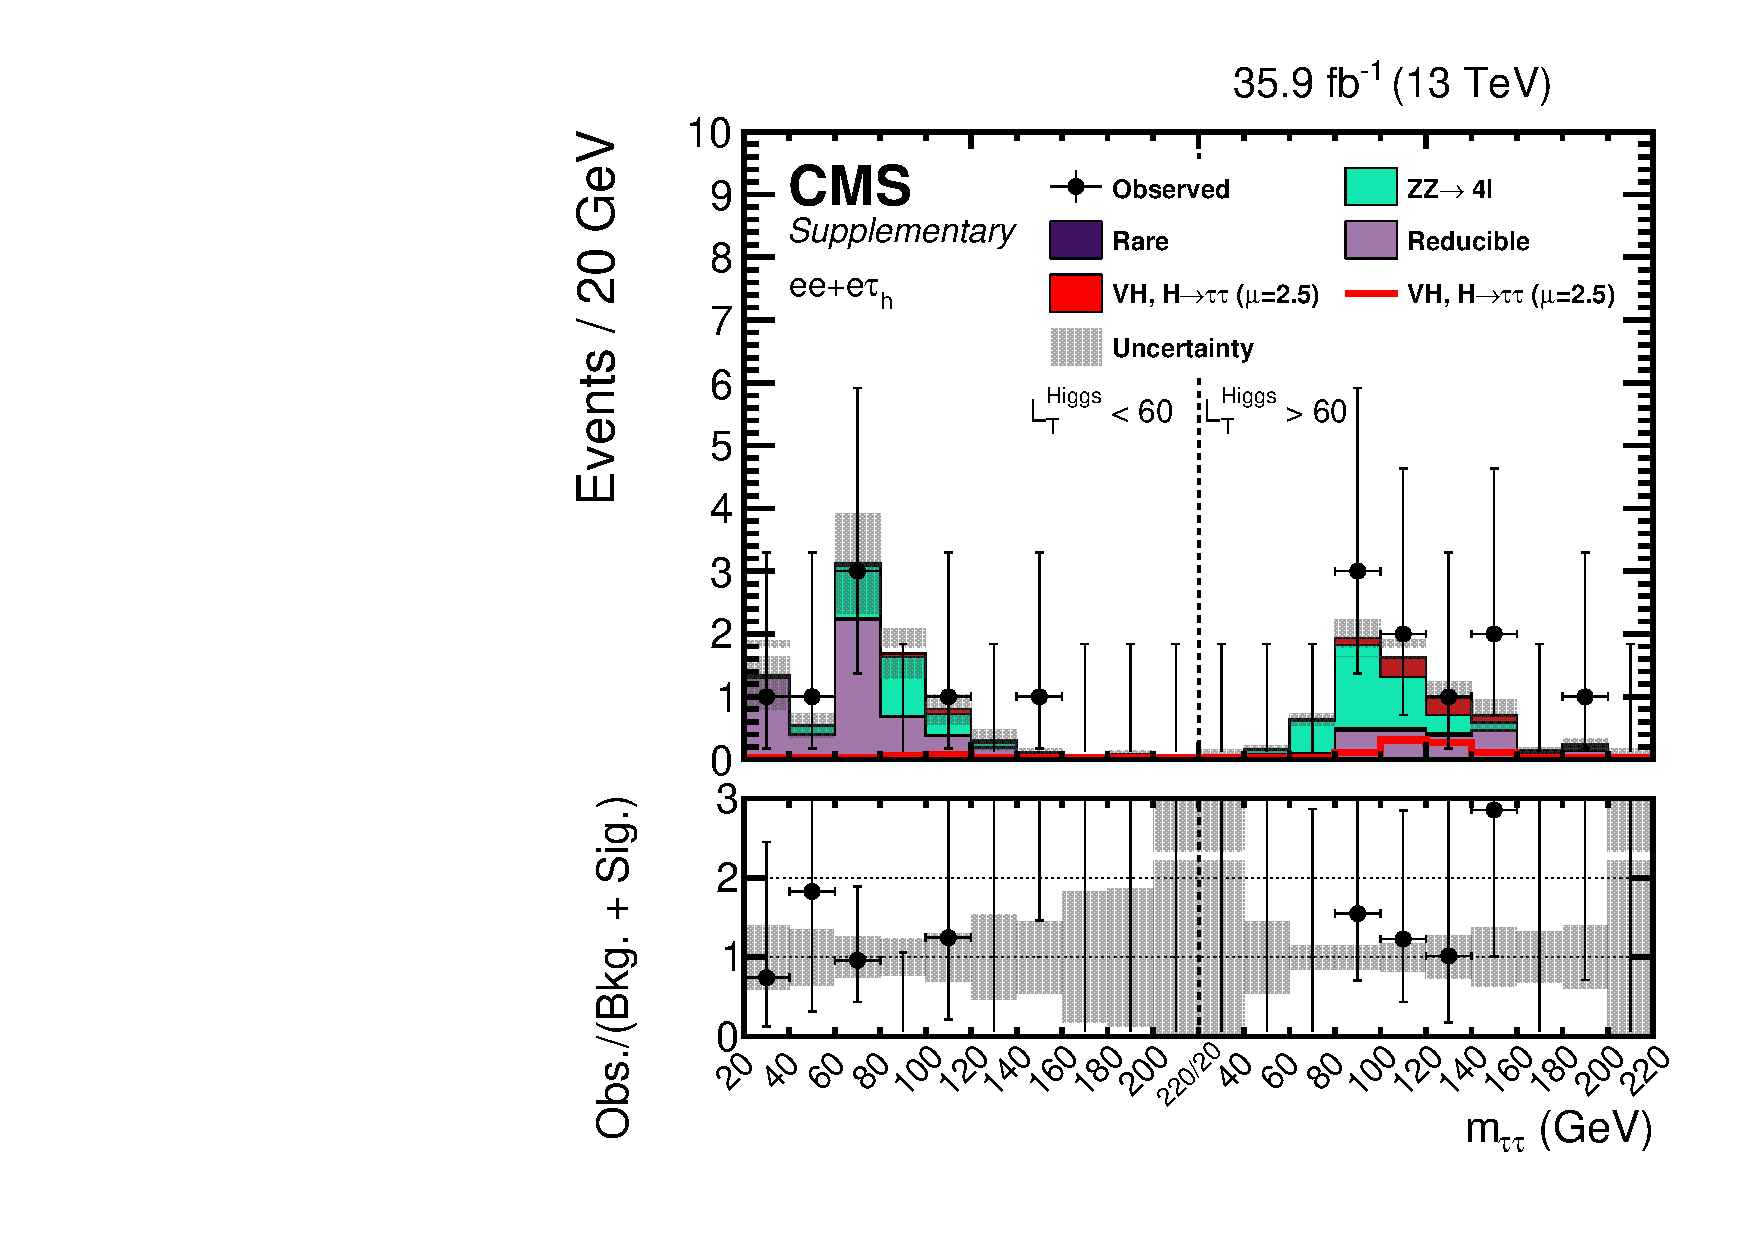
\includegraphics[width=0.49\textwidth]{higgs_to_taus_vh/plots/zh/eeet_postfit.pdf}
  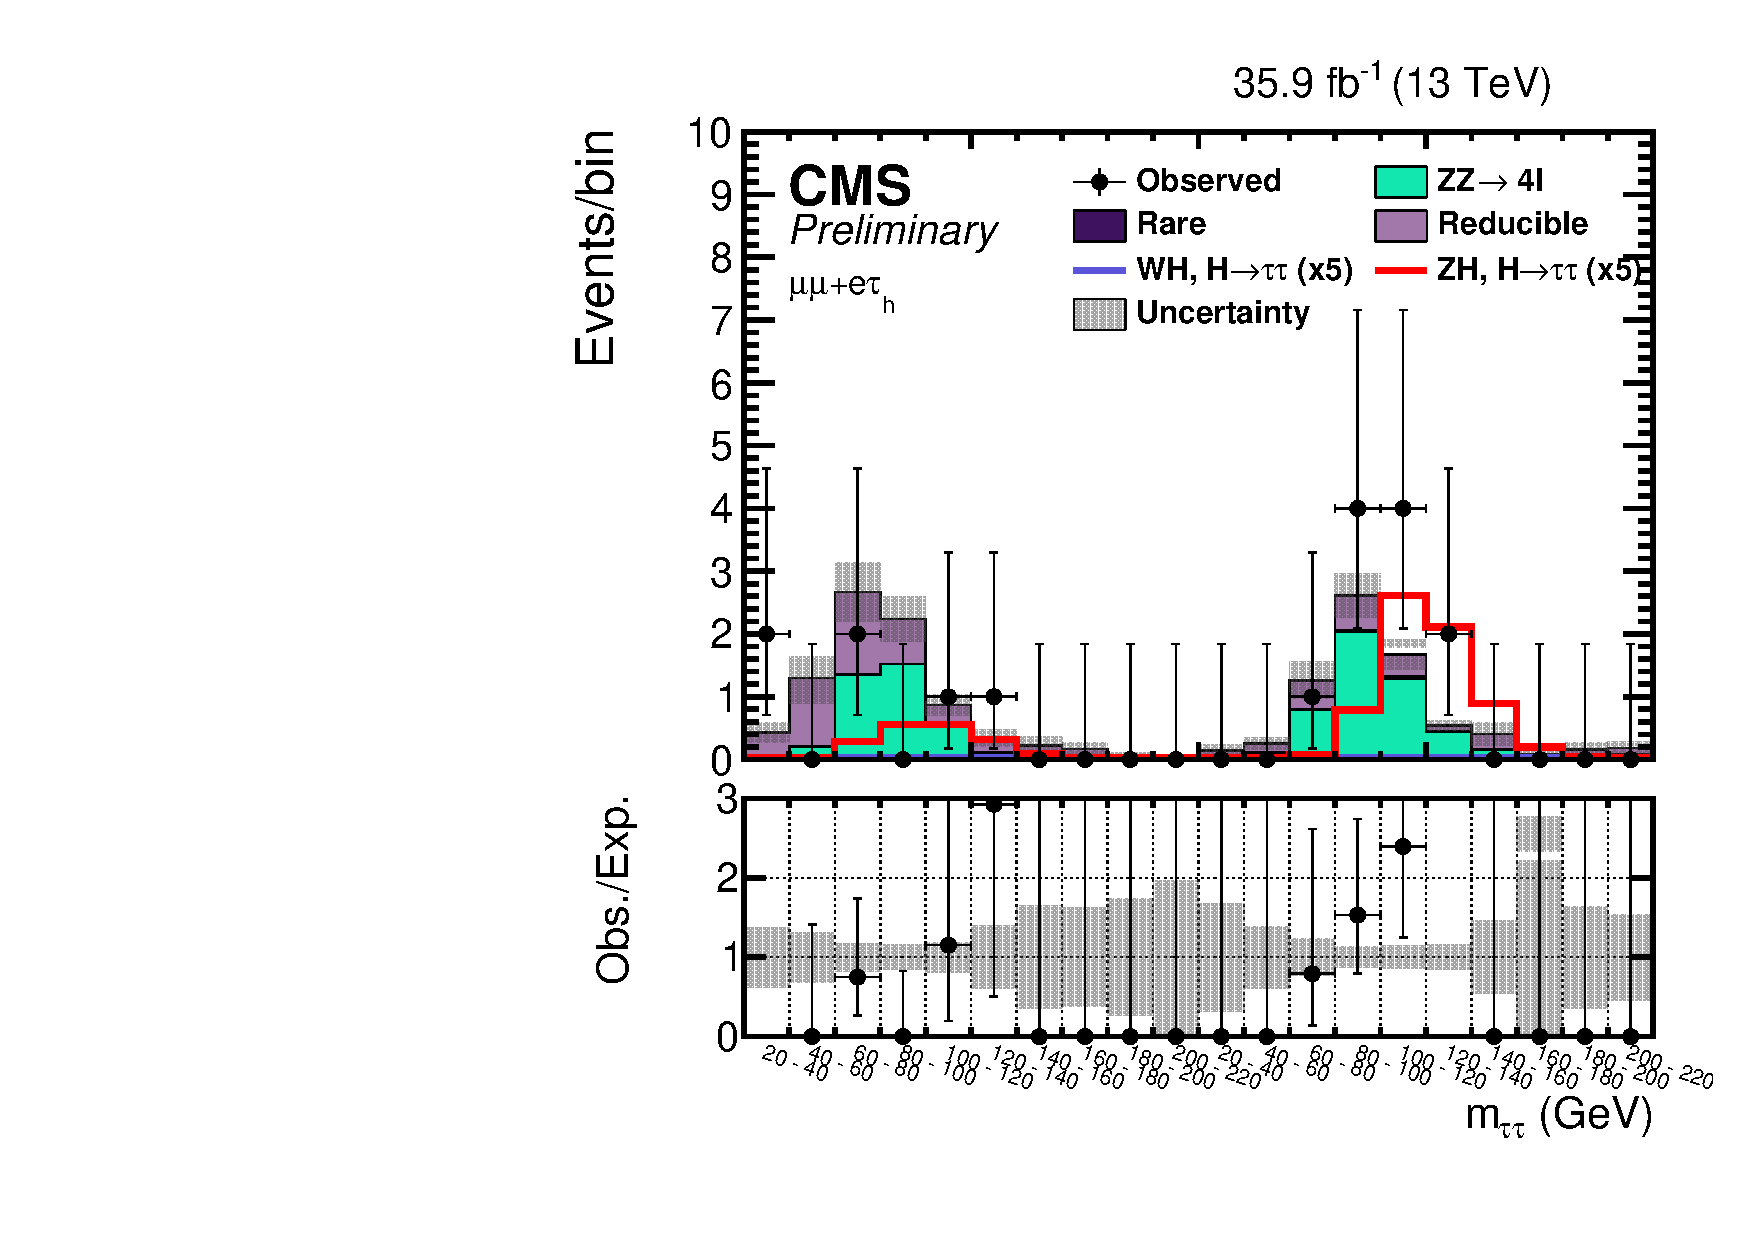
\includegraphics[width=0.49\textwidth]{higgs_to_taus_vh/plots/zh/emmt_postfit.pdf}
  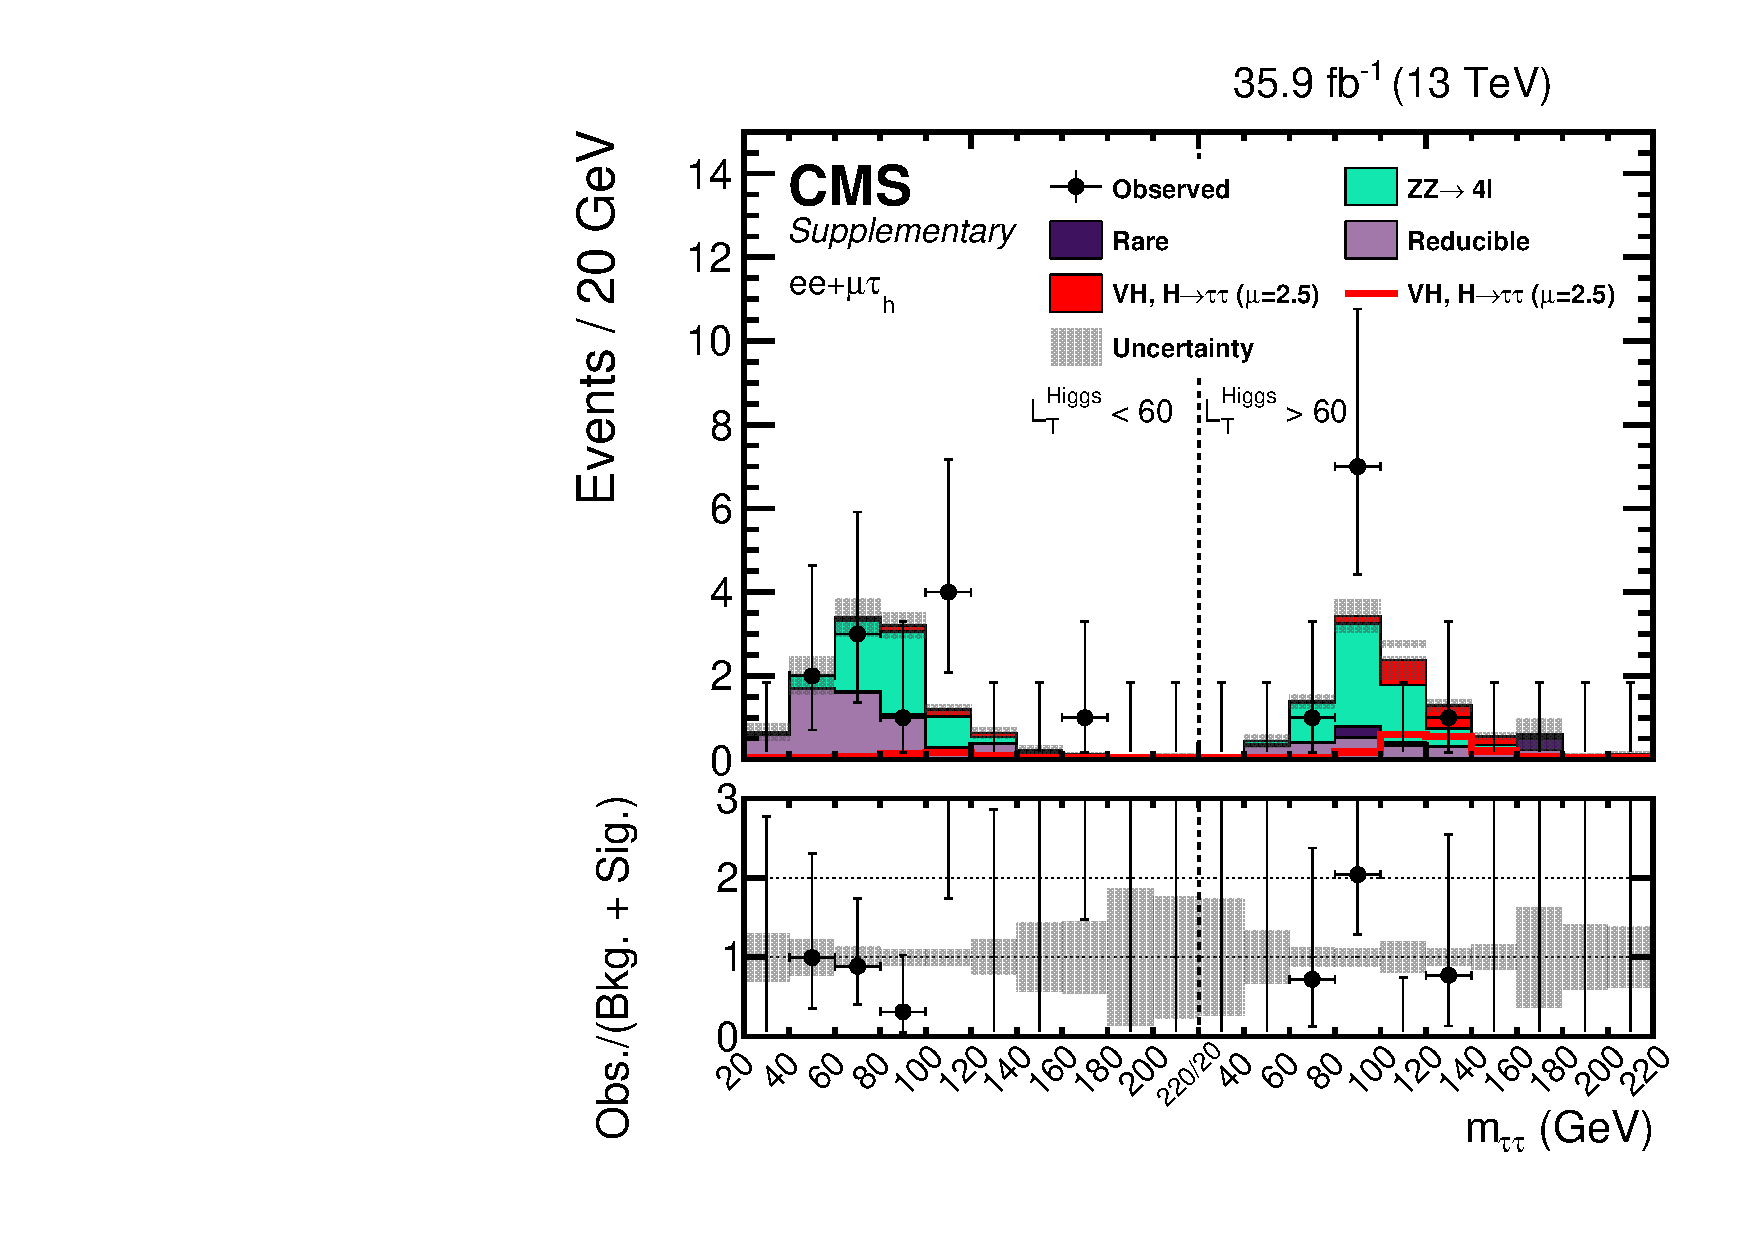
\includegraphics[width=0.49\textwidth]{higgs_to_taus_vh/plots/zh/eemt_postfit.pdf}
  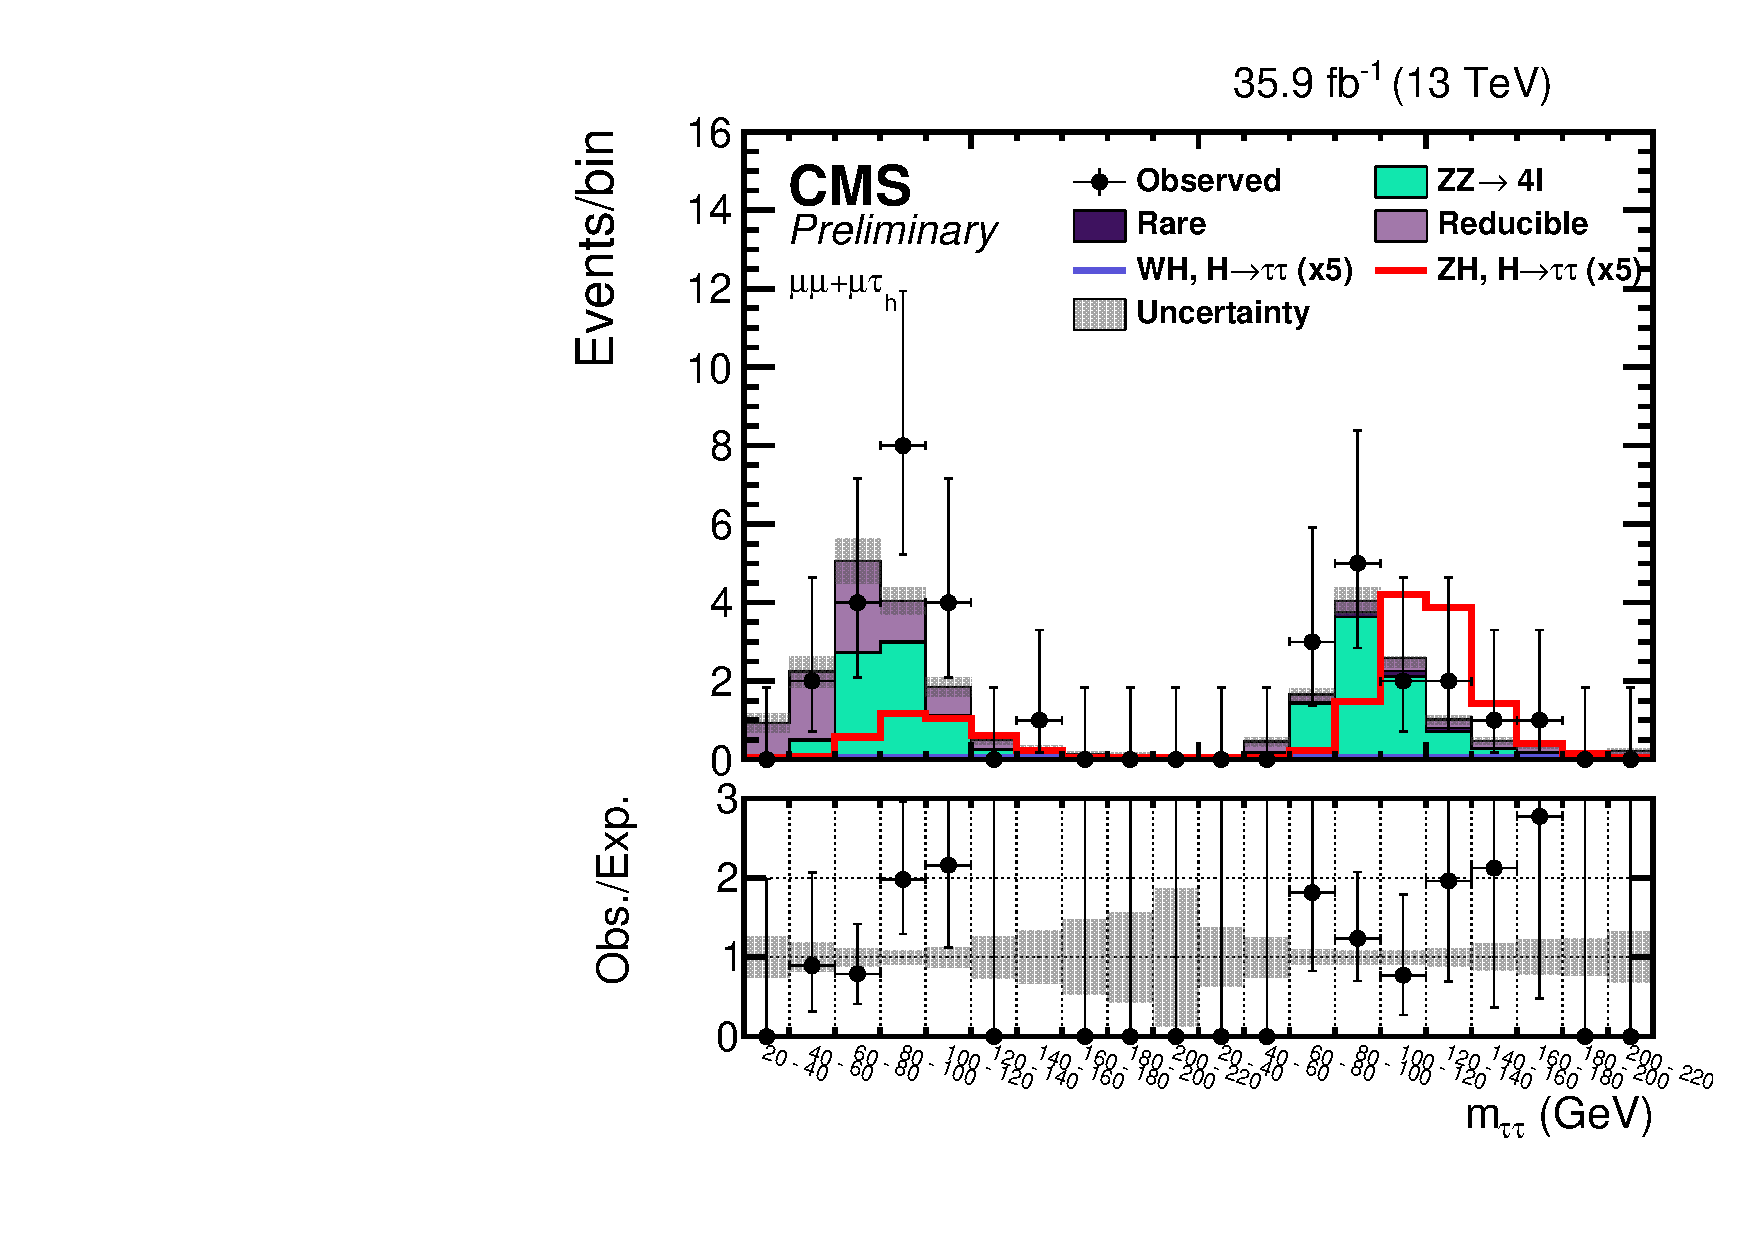
\includegraphics[width=0.49\textwidth]{higgs_to_taus_vh/plots/zh/mmmt_postfit.pdf}
 \end{center}
 \caption{The postfit $\mtt$ distributions used to extract the signal shown
  for the (top left) $\Pe\Pe\Pe\tauh$, (top right) $\Pgm\Pgm\Pe\tauh$, 
  (bottom left) $\Pe\Pe\Pgm\tauh$, and (bottom right) $\Pgm\Pgm\Pgm\tauh$
  final states. The distributions show full uncertainties.
  The $\PW\PH$ and $\PZ\PH$, $\htt$ signal processes are summed together and 
  shown as $\VH$, $\htt$ with a best-fit $\mu = 2.5$. $\VH$, $\htt$ is shown both as 
  a stacked filled histogram and an open overlaid histogram. In these distributions 
  the $\PZ\PH$, $\htt$ process contributes more than 99\% of the total of $\VH$, $\htt$.
 }
 \label{fig:zh_all_eight1}
\end{figure}

\begin{figure}[h!]
 \begin{center}
  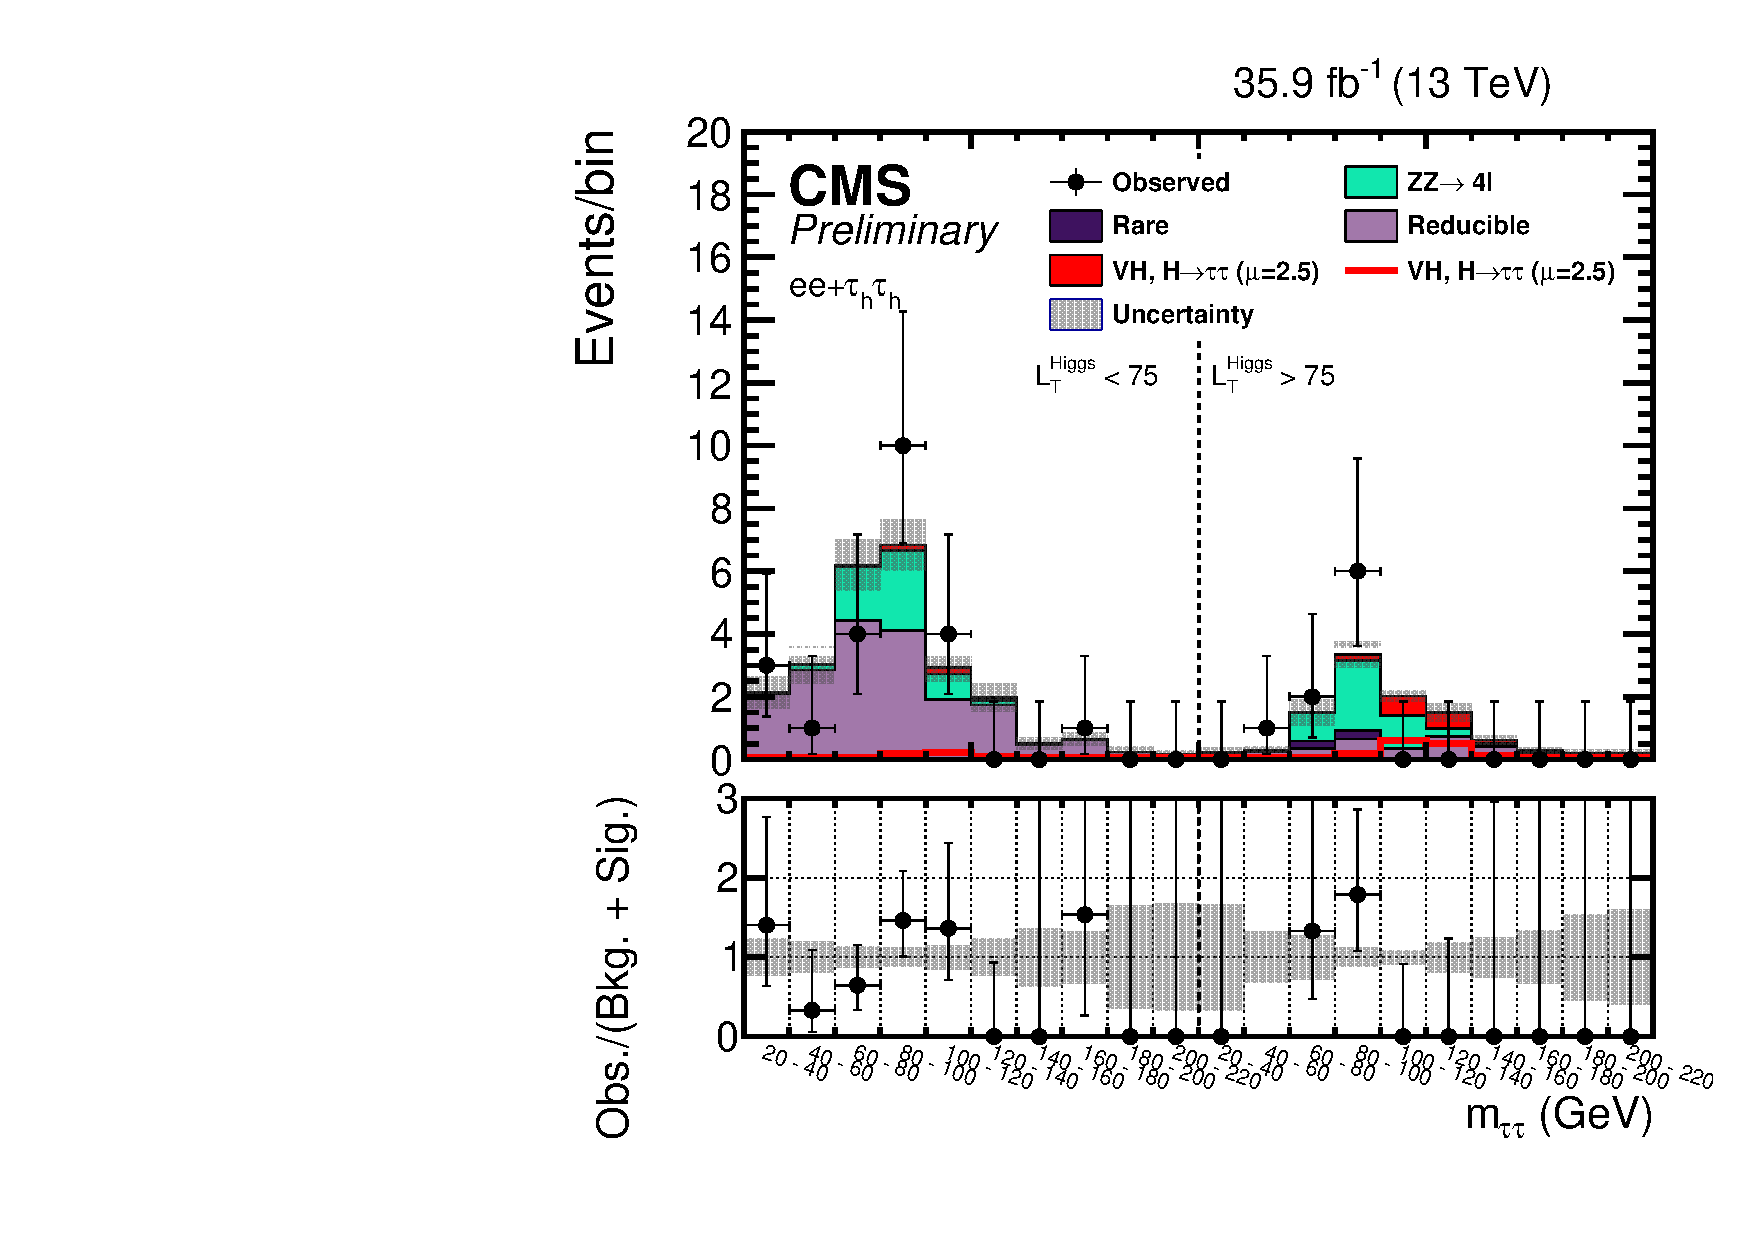
\includegraphics[width=0.49\textwidth]{higgs_to_taus_vh/plots/zh/eett_postfit.pdf}
  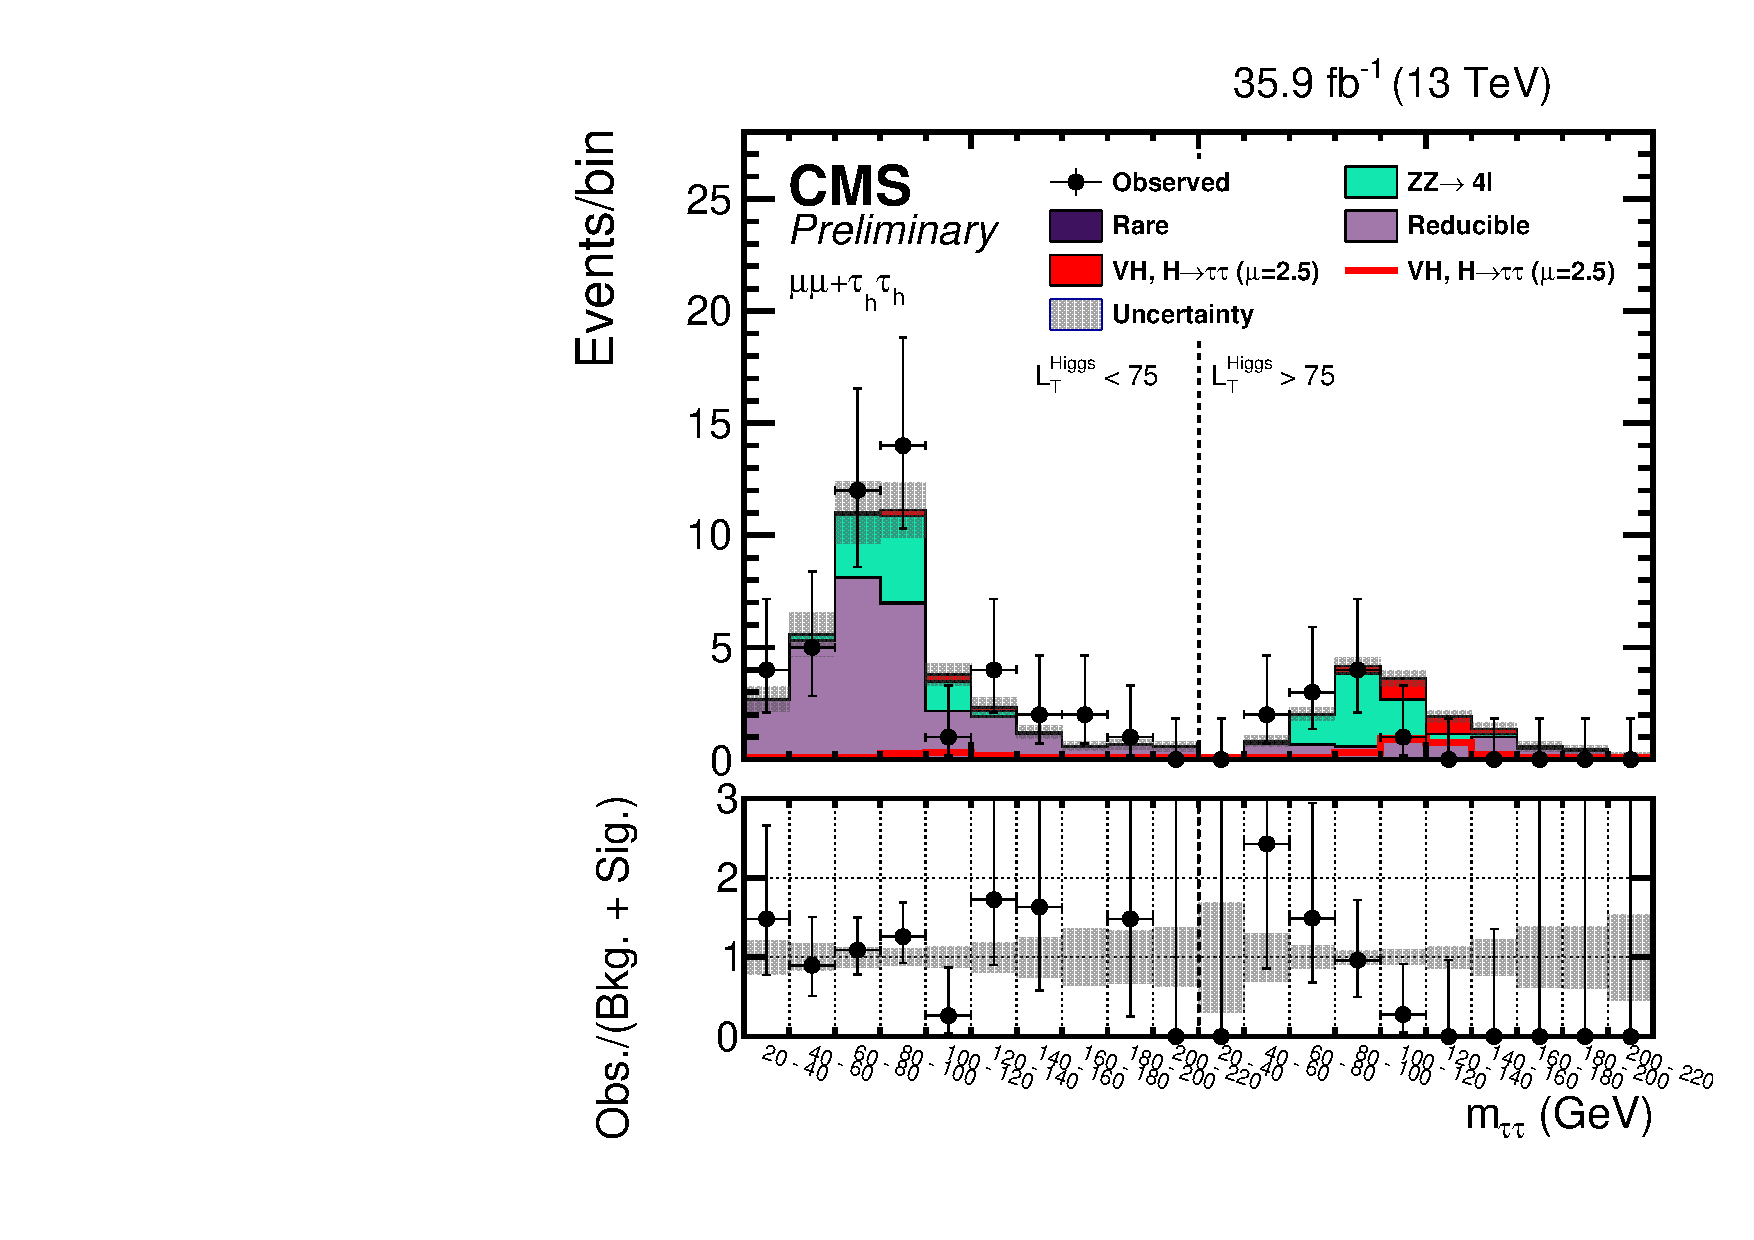
\includegraphics[width=0.49\textwidth]{higgs_to_taus_vh/plots/zh/mmtt_postfit.pdf}
  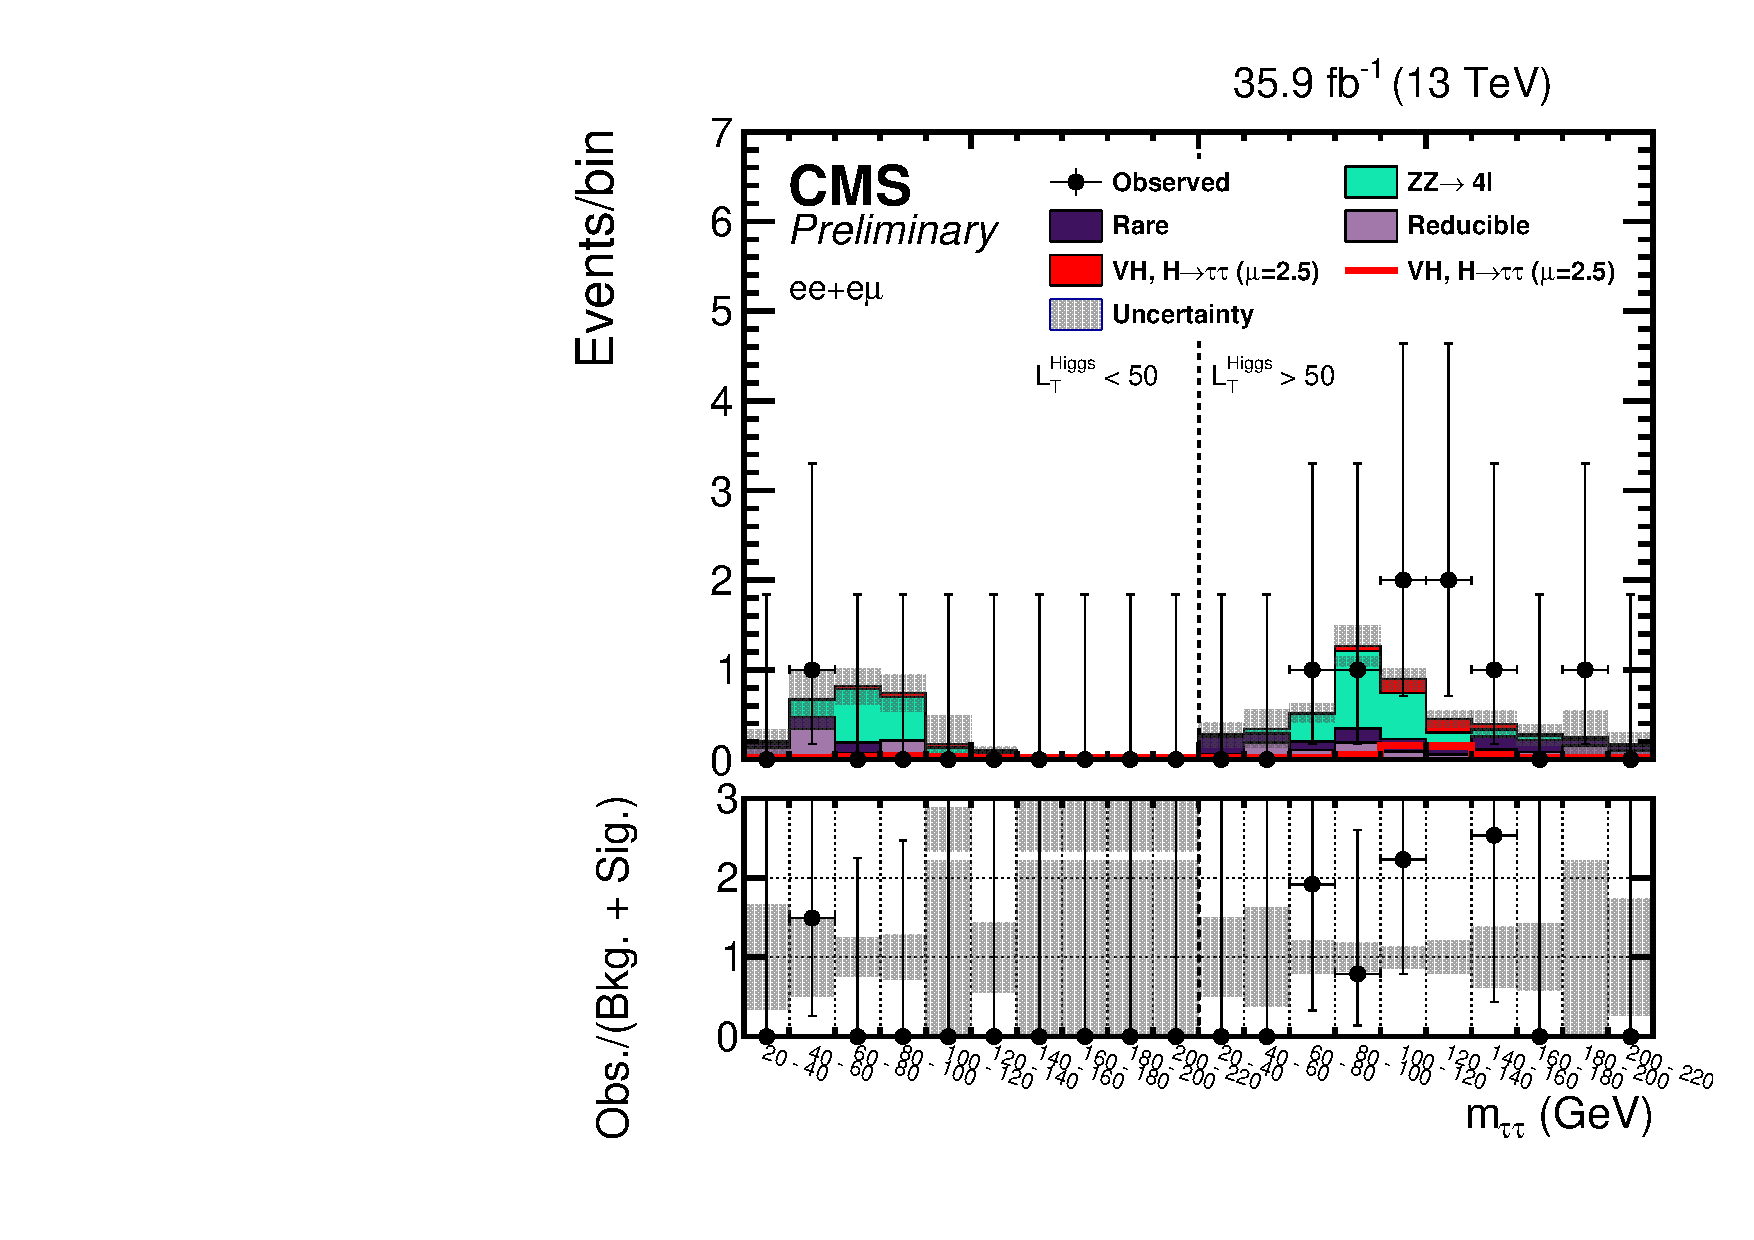
\includegraphics[width=0.49\textwidth]{higgs_to_taus_vh/plots/zh/eeem_postfit.pdf}
  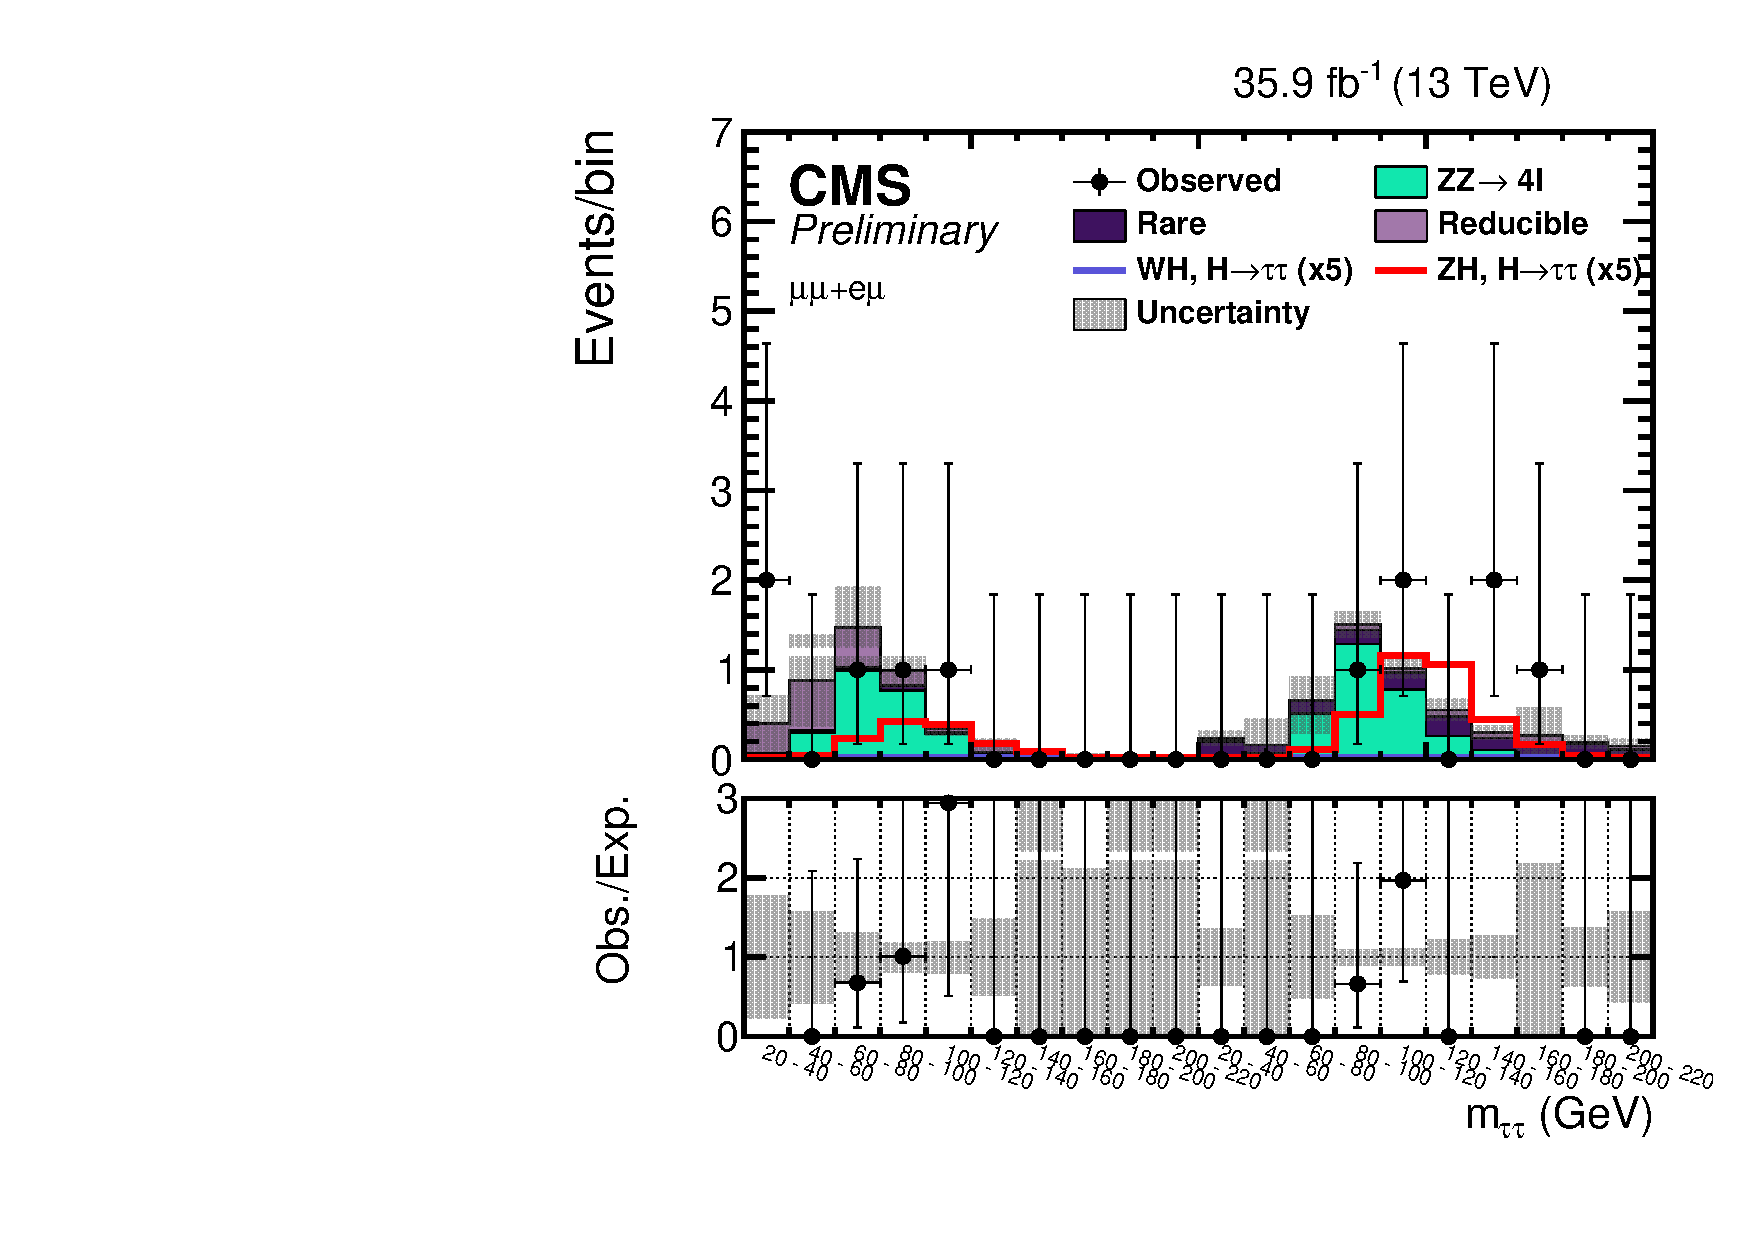
\includegraphics[width=0.49\textwidth]{higgs_to_taus_vh/plots/zh/emmm_postfit.pdf}
 \end{center}
 \caption{The postfit $\mtt$ distributions used to extract the signal shown
  for the (top left) $\Pe\Pe\tauh\tauh$, (top right) $\Pgm\Pgm\tauh\tauh$, 
  (bottom left) $\Pe\Pe\Pe\Pgm$, and (bottom right) $\Pgm\Pgm\Pe\Pgm$
  final states. The distributions show full uncertainties.
  The $\PW\PH$ and $\PZ\PH$, $\htt$ signal processes are summed together and 
  shown as $\VH$, $\htt$ with a best-fit $\mu = 2.5$. $\VH$, $\htt$ is shown both as 
  a stacked filled histogram and an open overlaid histogram. In these distributions 
  the $\PZ\PH$, $\htt$ process contributes more than 99\% of the total of $\VH$, $\htt$.
 }
 \label{fig:zh_all_eight2}
\end{figure}

%\begin{figure}[h!]
% \begin{center}
%  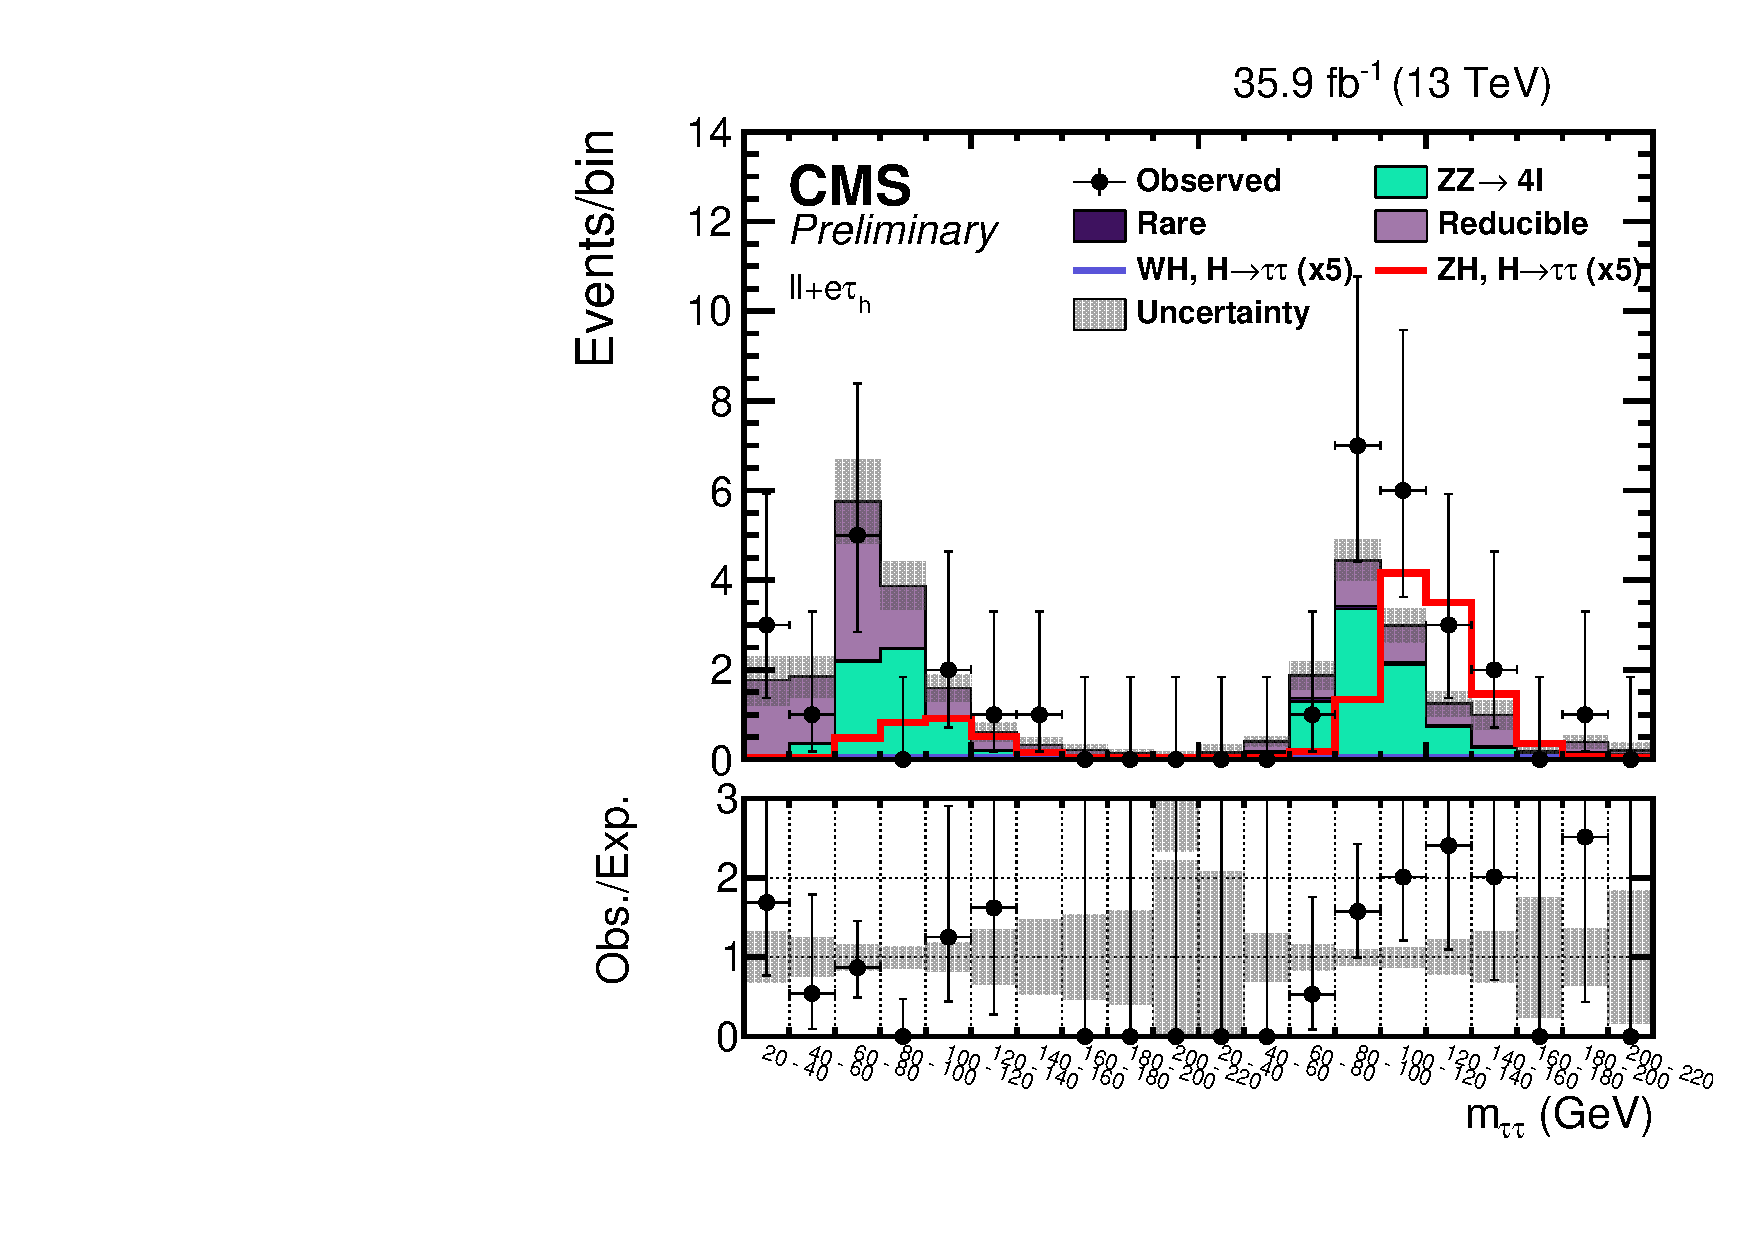
\includegraphics[width=0.45\textwidth]{higgs_to_taus_vh/plots/zh/llet_postfit.pdf}
%  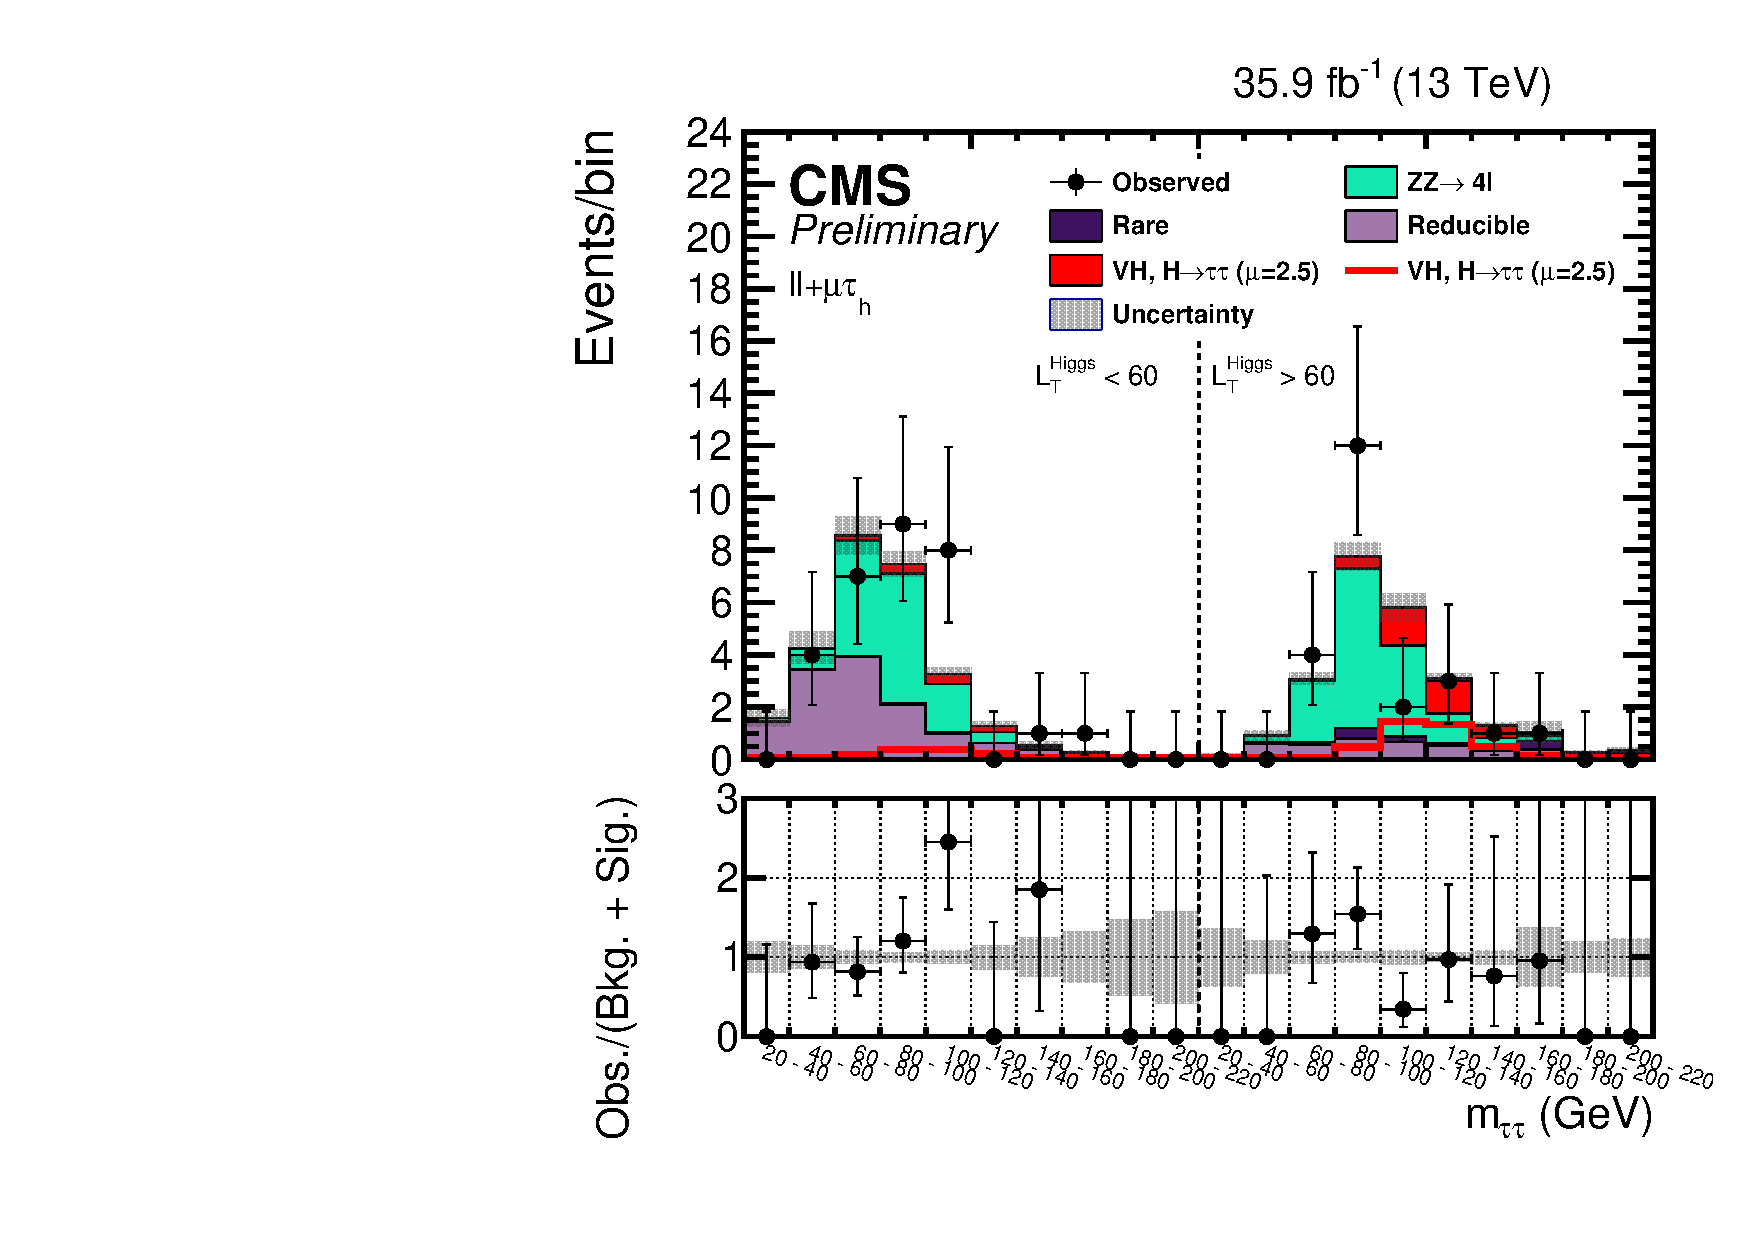
\includegraphics[width=0.45\textwidth]{higgs_to_taus_vh/plots/zh/llmt_postfit.pdf}
%  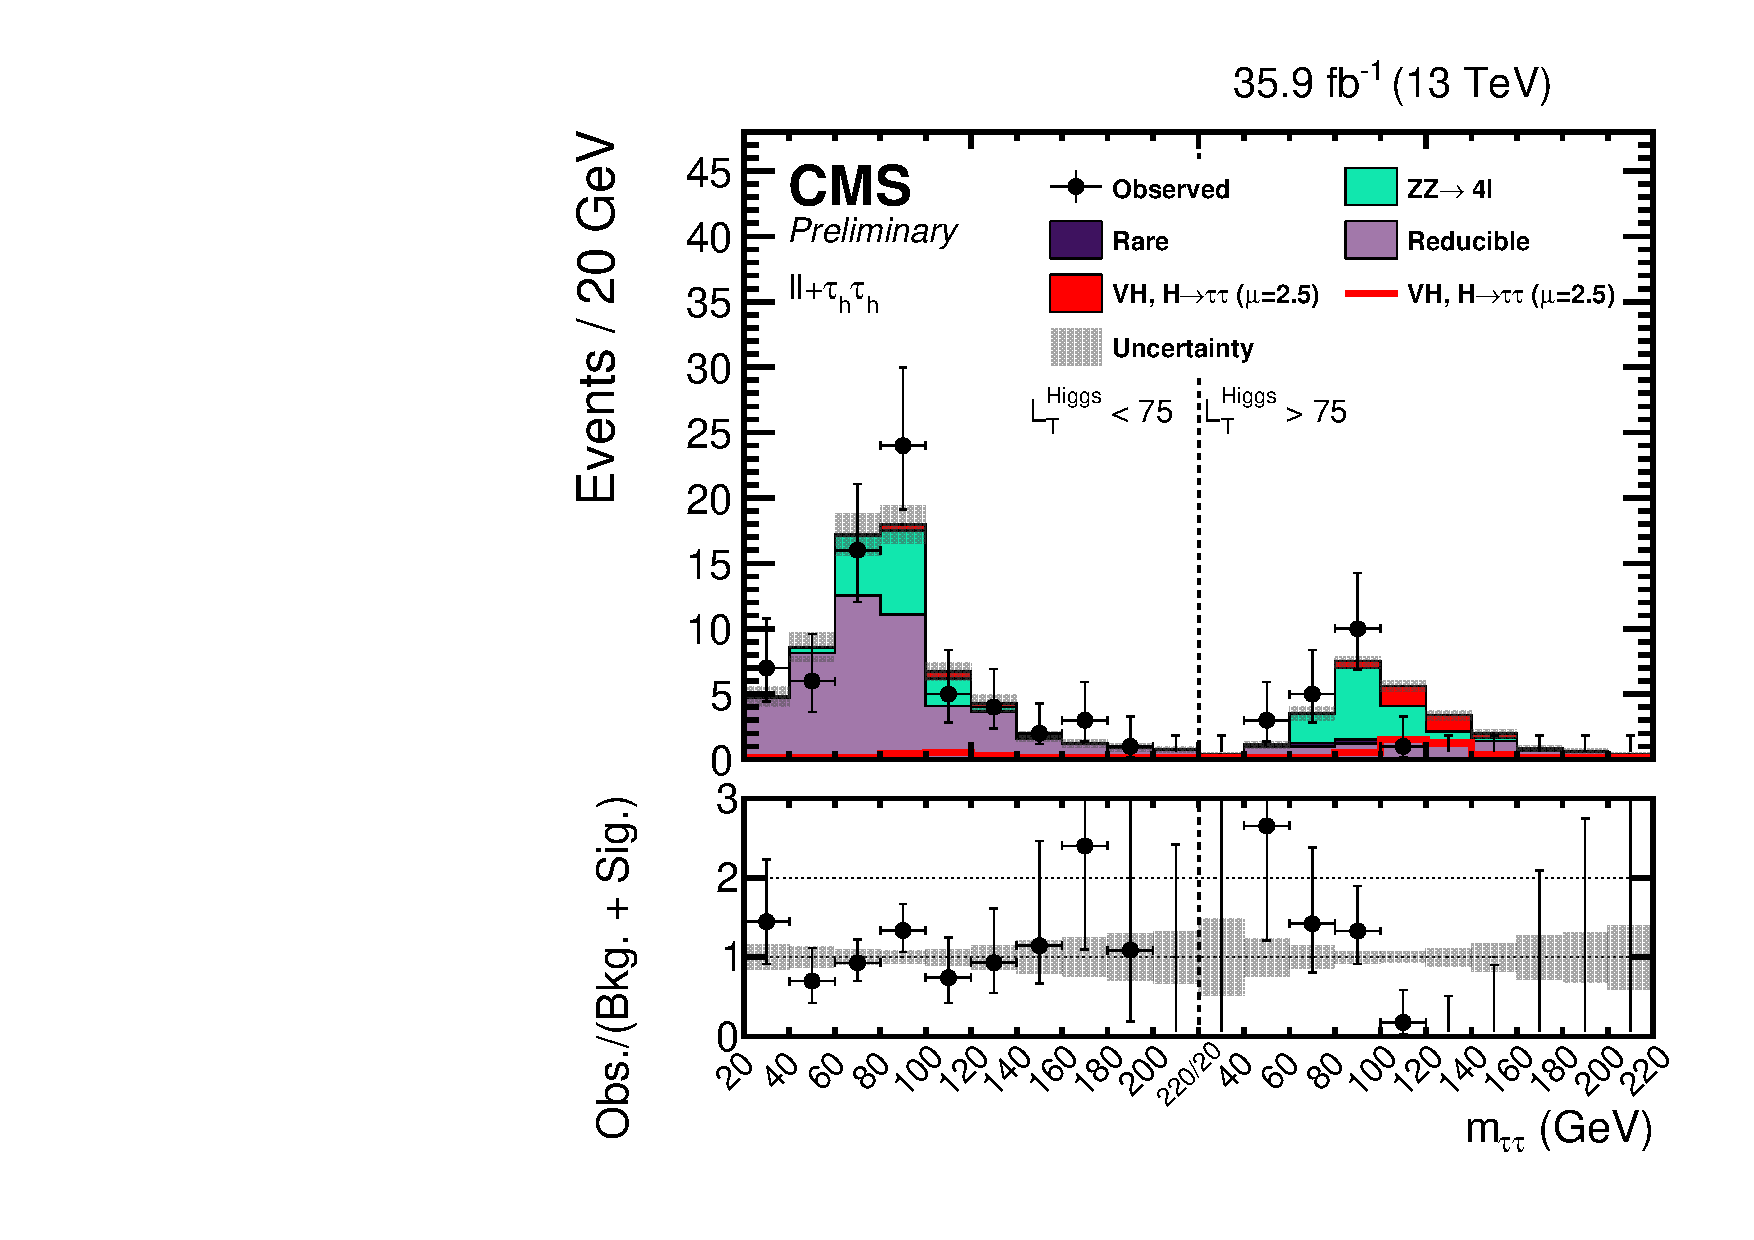
\includegraphics[width=0.45\textwidth]{higgs_to_taus_vh/plots/zh/lltt_postfit.pdf}
%  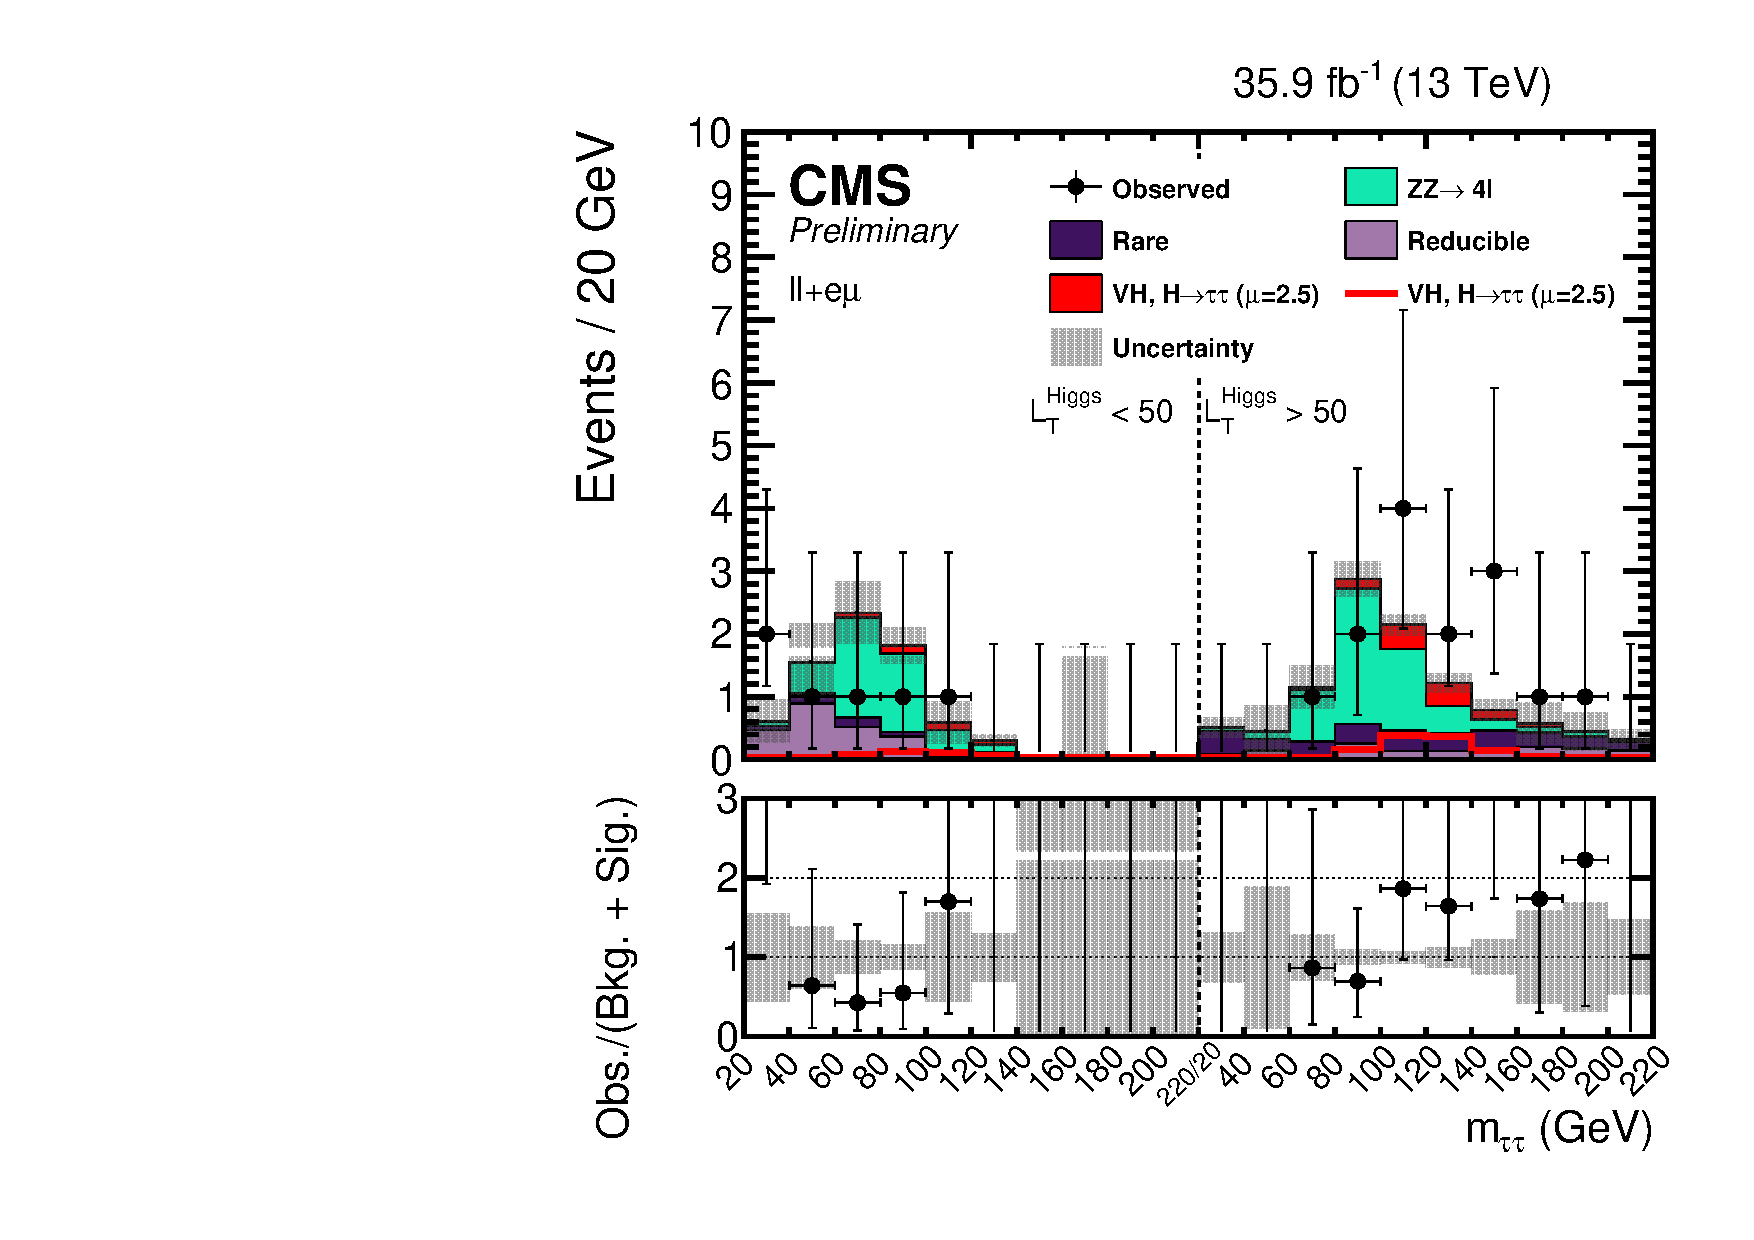
\includegraphics[width=0.45\textwidth]{higgs_to_taus_vh/plots/zh/llem_postfit.pdf}
% \end{center}
% \caption{The postfit $\mtt$ distributions used to extract the signal shown
%  for (top left) $\ell\ell\Pe\tauh$, (top right) $\ell\ell\Pgm\tauh$, 
%  (bottom left) $\ell\ell\tauh\tauh$, and (bottom right) $\ell\ell\Pe\Pgm$.
%  The left half of each distribution is the Low-$L_{\text{T}}^{\textrm{Higgs}}$ region
%  while the right half of each distribution is the High-$L_{\text{T}}^{\textrm{Higgs}}$ region.
%  $\ell\ell$ covers both $\PZ \to \Pgm\Pgm$ and $\PZ \to \Pe\Pe$ events.
%  The distributions show full uncertainties.
%  The $\PW\PH$ and $\PZ\PH$, $\htt$ signal processes are summed together and 
%  shown as $\VH$, $\htt$ with a best-fit $\mu = 2.5$. $\VH$, $\htt$ is shown both as 
%  a stacked filled histogram and an open overlaid histogram. In these distributions 
%  the $\PZ\PH$, $\htt$ process contributes more than 99\% of the total of $\VH$, $\htt$.
% }
% \label{fig:zh_results_svFitLLXX}
%\end{figure}


\begin{figure}[h!]
 \begin{center}
  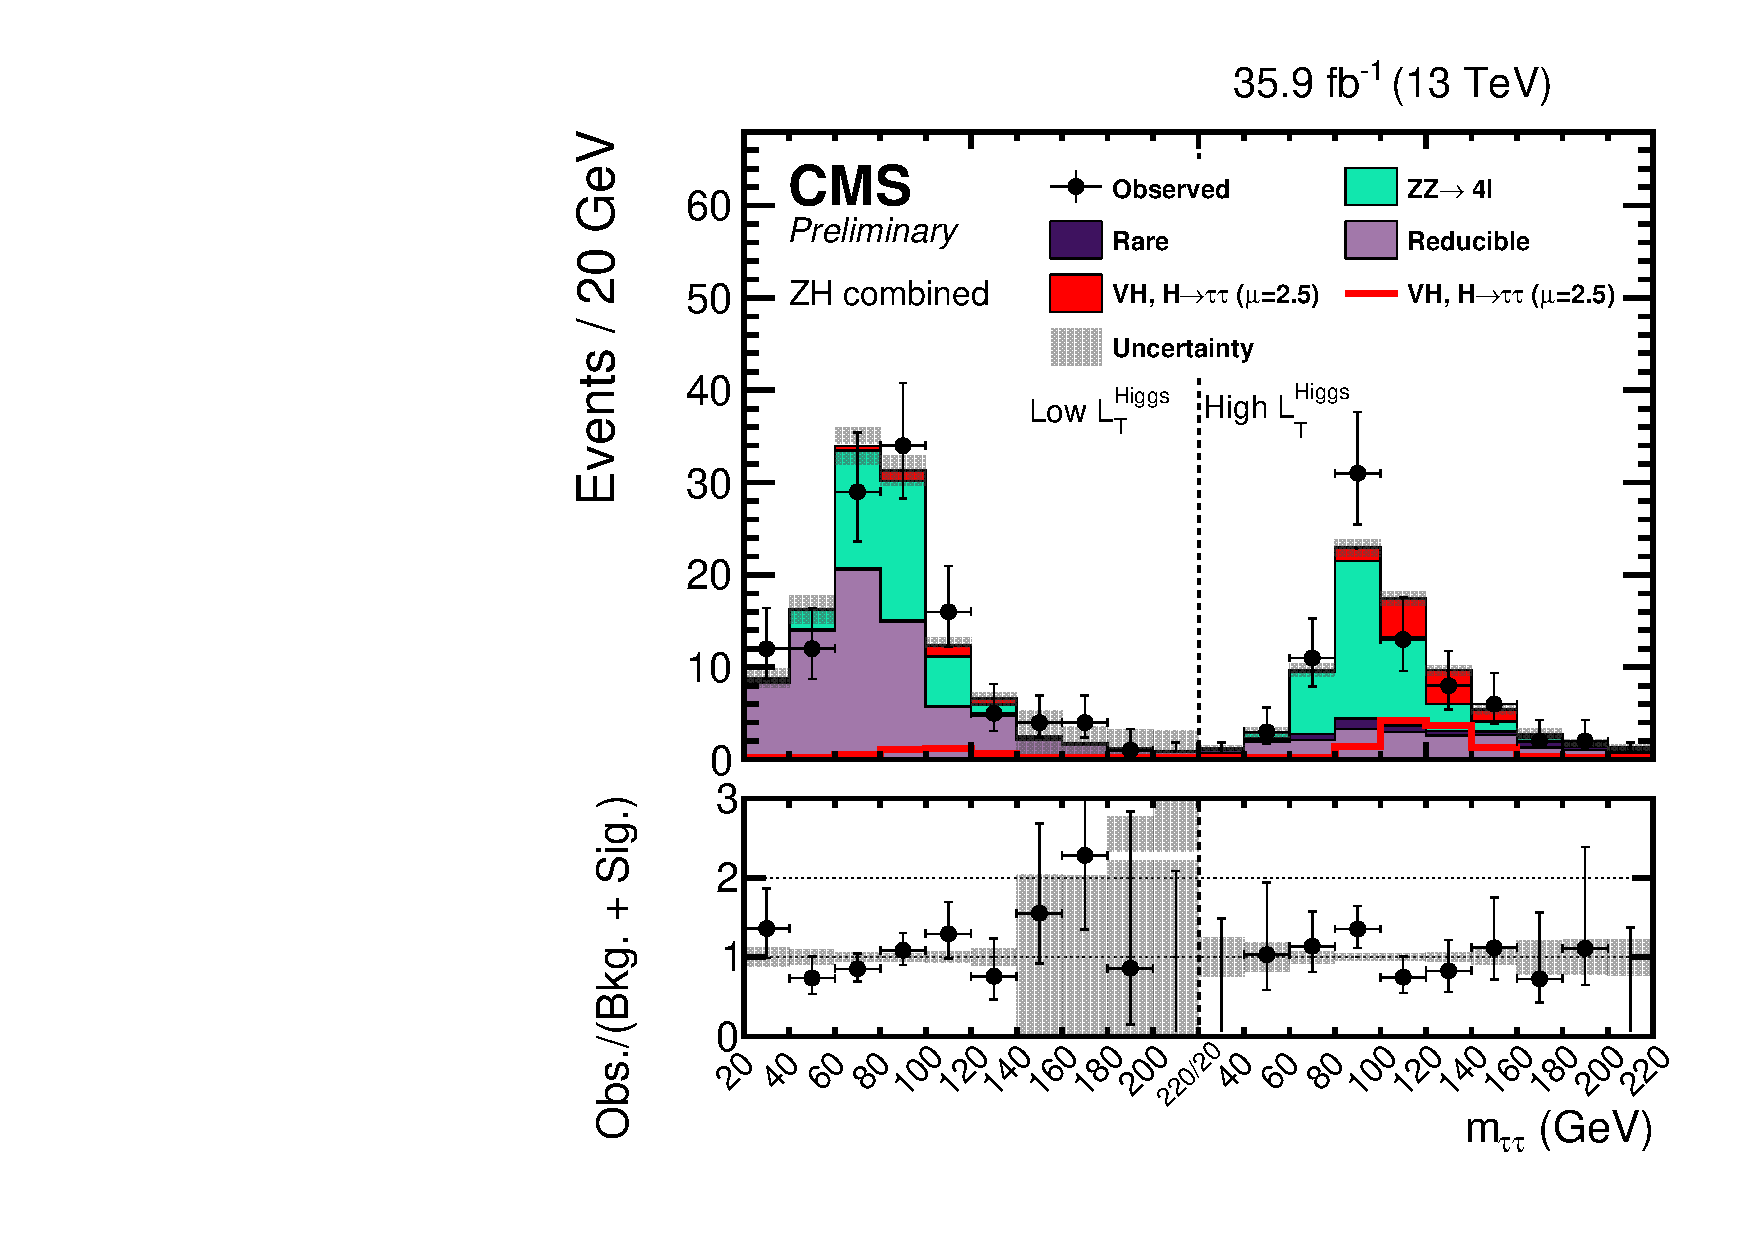
\includegraphics[width=0.65\textwidth]{higgs_to_taus_vh/plots/zh/zh_postfit.pdf}
 \end{center}
 \caption{The postfit $\mtt$ distributions used to extract the signal shown
  for all 8 $\PZ\PH$ final states combined.
  The distribution shows full uncertainties.
  The left half of the distribution is the Low-$L_{\text{T}}^{\textrm{Higgs}}$ region
  while the right half corresponds to the High-$L_{\text{T}}^{\textrm{Higgs}}$ region.
  The definitions of the $L_{\text{T}}^{\textrm{Higgs}}$ regions in this distribution 
  are the same as those used in Figures~\ref{fig:zh_all_eight1} 
  and ~\ref{fig:zh_all_eight2} and are final state dependent.
  The $\PW\PH$ and $\PZ\PH$, $\htt$ signal processes are summed together and 
  shown as $\VH$, $\htt$ with a best-fit $\mu = 2.5$. $\VH$, $\htt$ is shown both as 
  a stacked filled histogram and an open overlaid histogram. In this distribution 
  the $\PZ\PH$, $\htt$ process contributes more than 99\% of the total of $\VH$, $\htt$.
 }
 \label{fig:zh_results_svFitAll}
\end{figure}



The results in the $\PW\PH$ final states are obtained from the distributions of the 
visible mass of the $\tauh$ leptons in the hadronic $\ell\tauh\tauh$ final states, 
and of the visible mass of the $\tauh$ and subleading light lepton in the 
semileptonic $\ell\ell\tauh$ final states. The mass distributions
are shown in Figure~\ref{fig:mass_whs} for the four $\PW\PH$ final states. 
Figure~\ref{fig:mass_wh} shows all four $\PW\PH$ final states combined together
for visualization purposes only.

\begin{figure}[h!]
 \begin{center}
  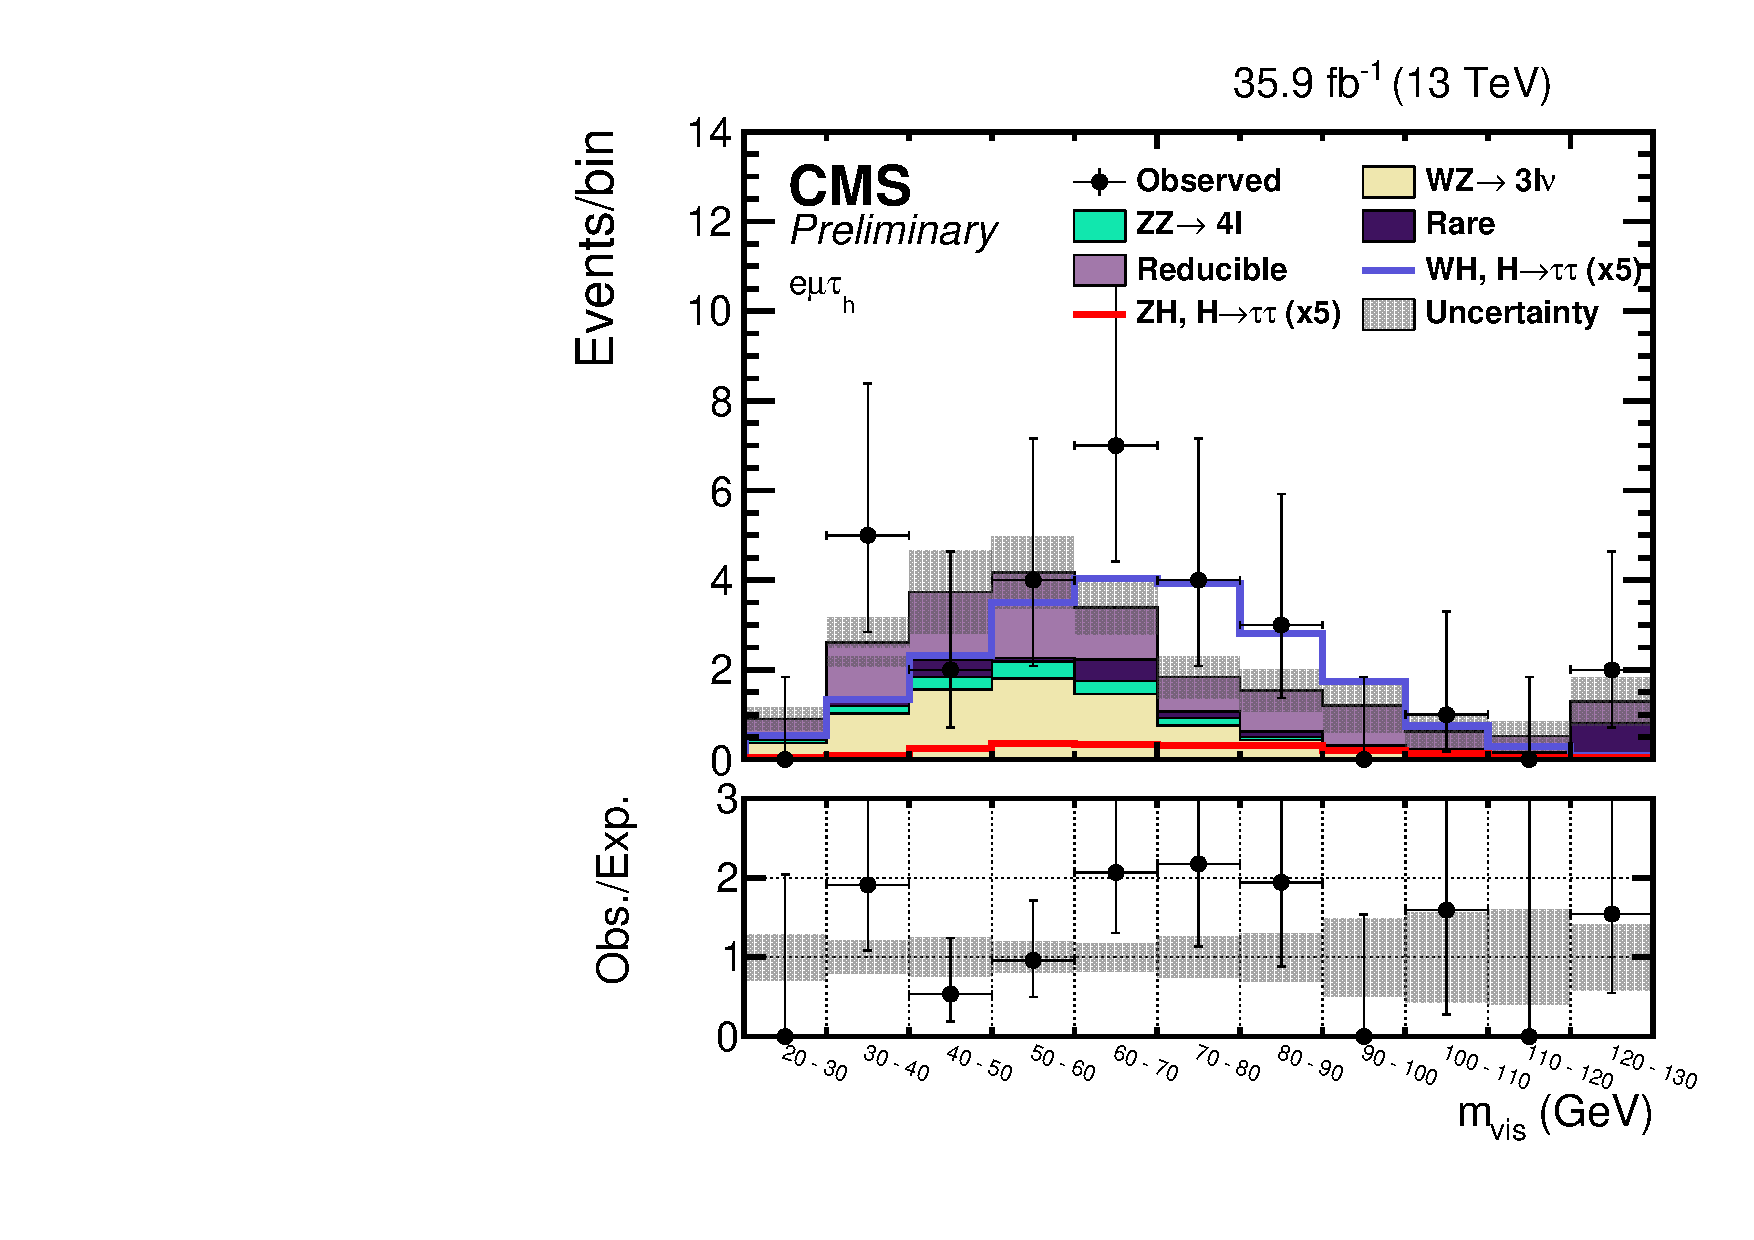
\includegraphics[width=0.49\textwidth]{higgs_to_taus_vh/plots/wh/emt_postfit.pdf}
  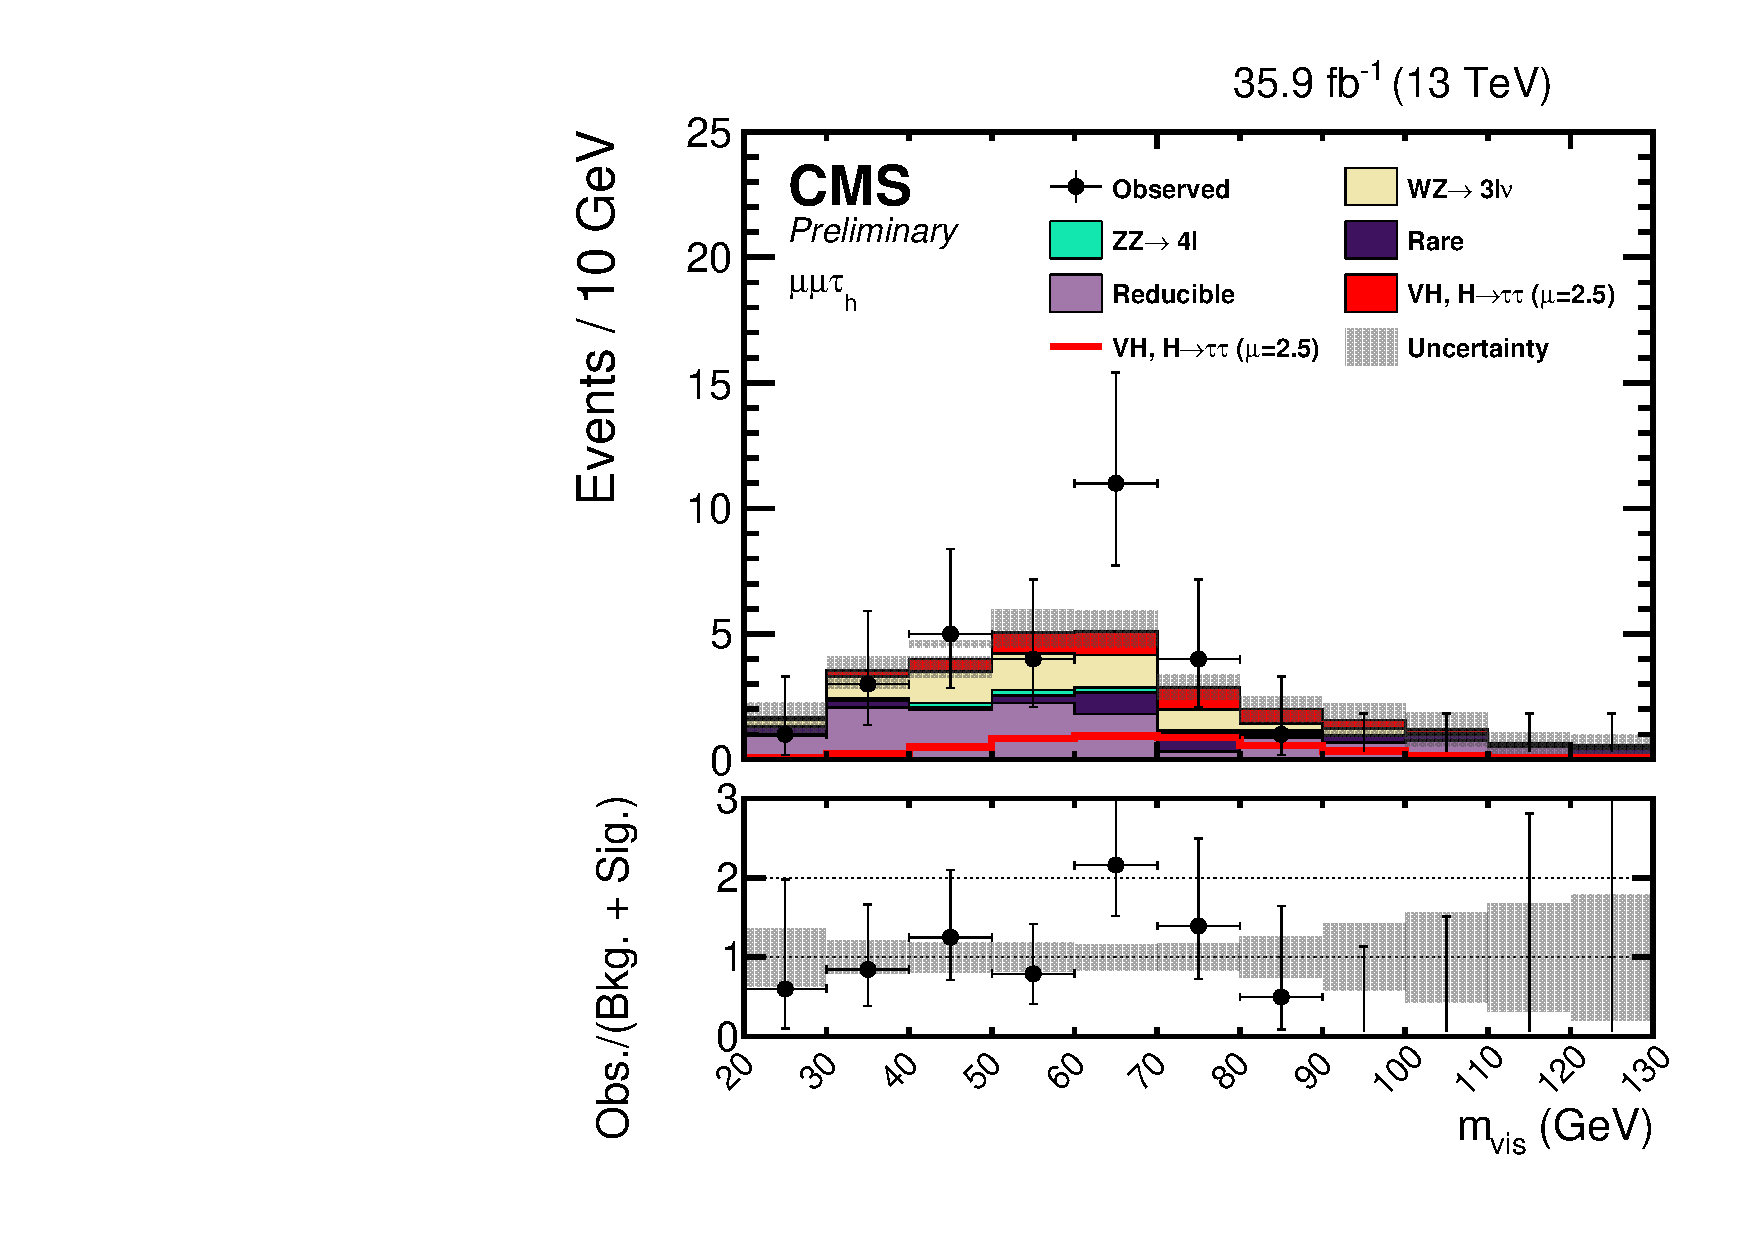
\includegraphics[width=0.49\textwidth]{higgs_to_taus_vh/plots/wh/mmt_postfit.pdf}
  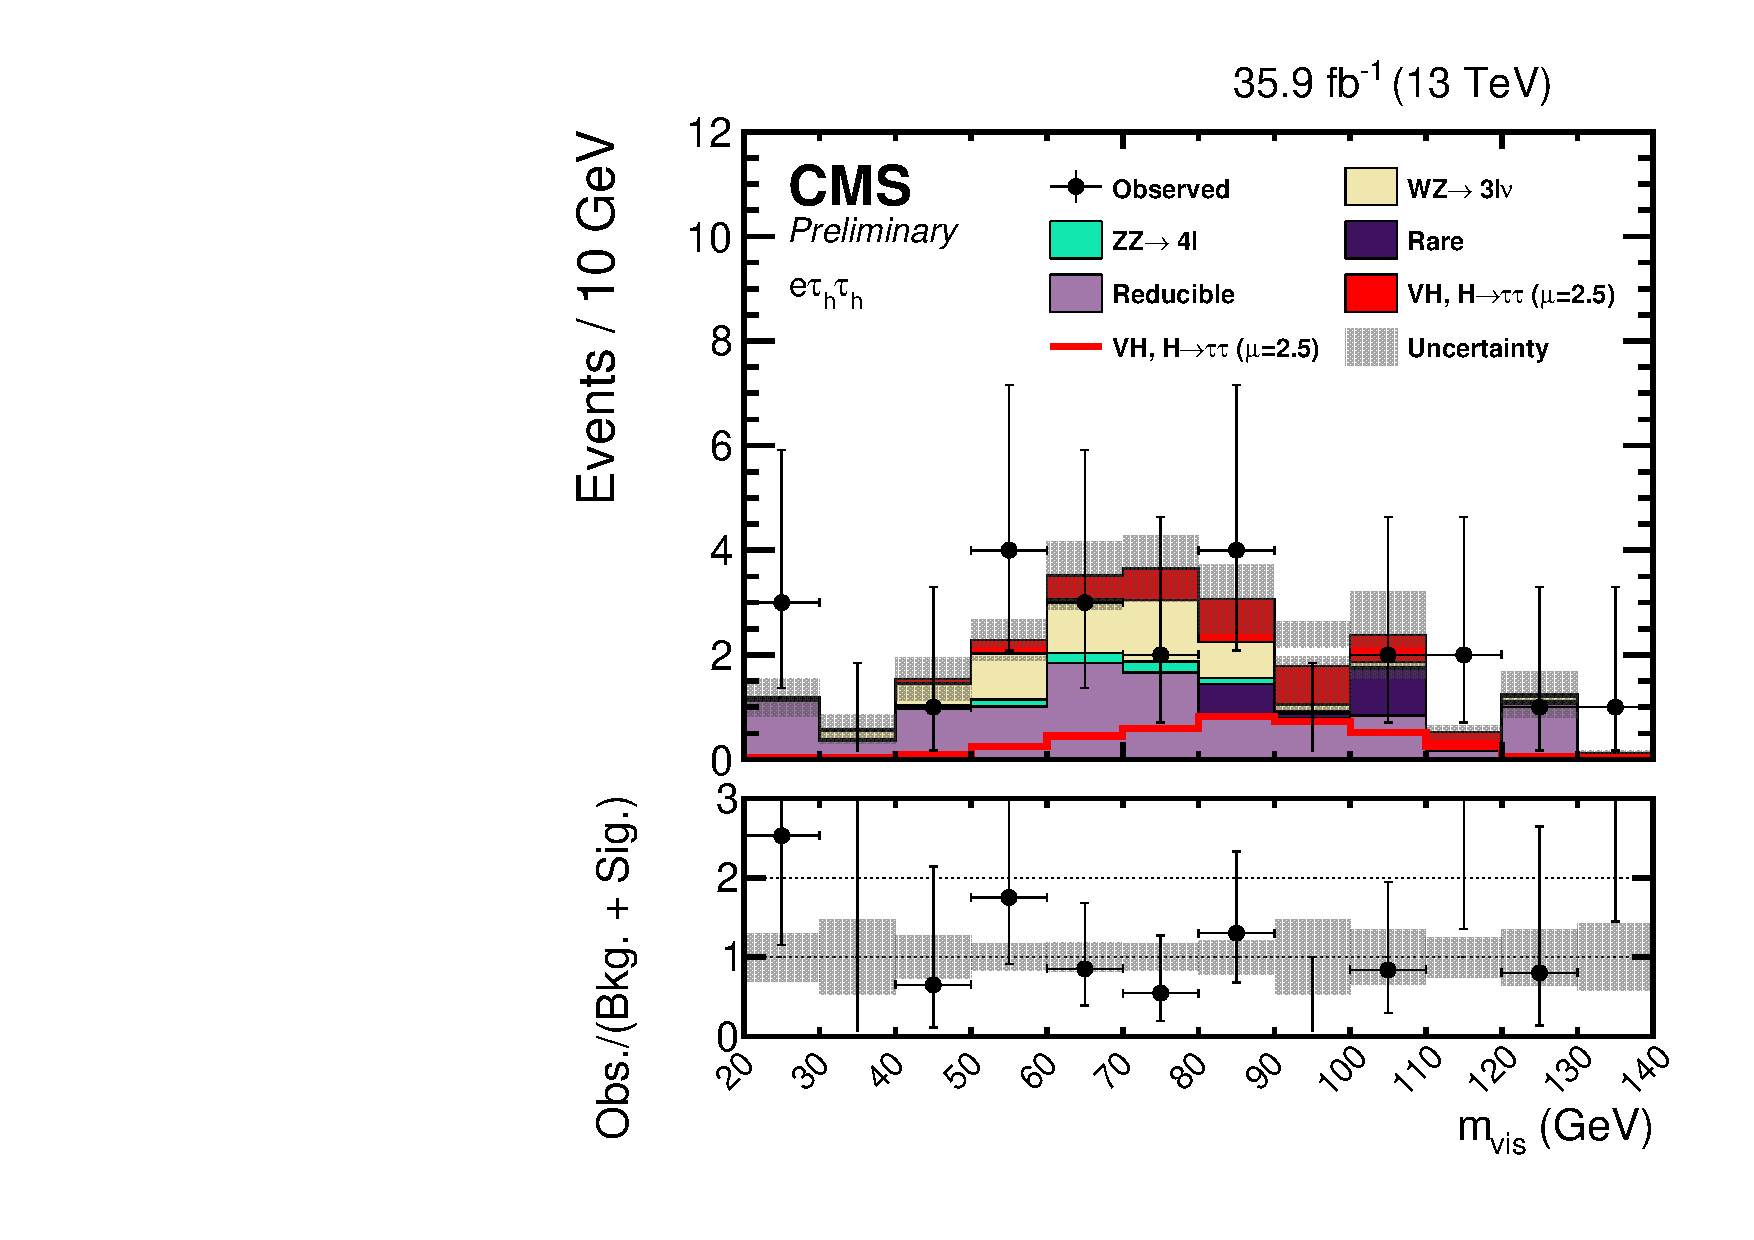
\includegraphics[width=0.49\textwidth]{higgs_to_taus_vh/plots/wh/ett_postfit.pdf}
  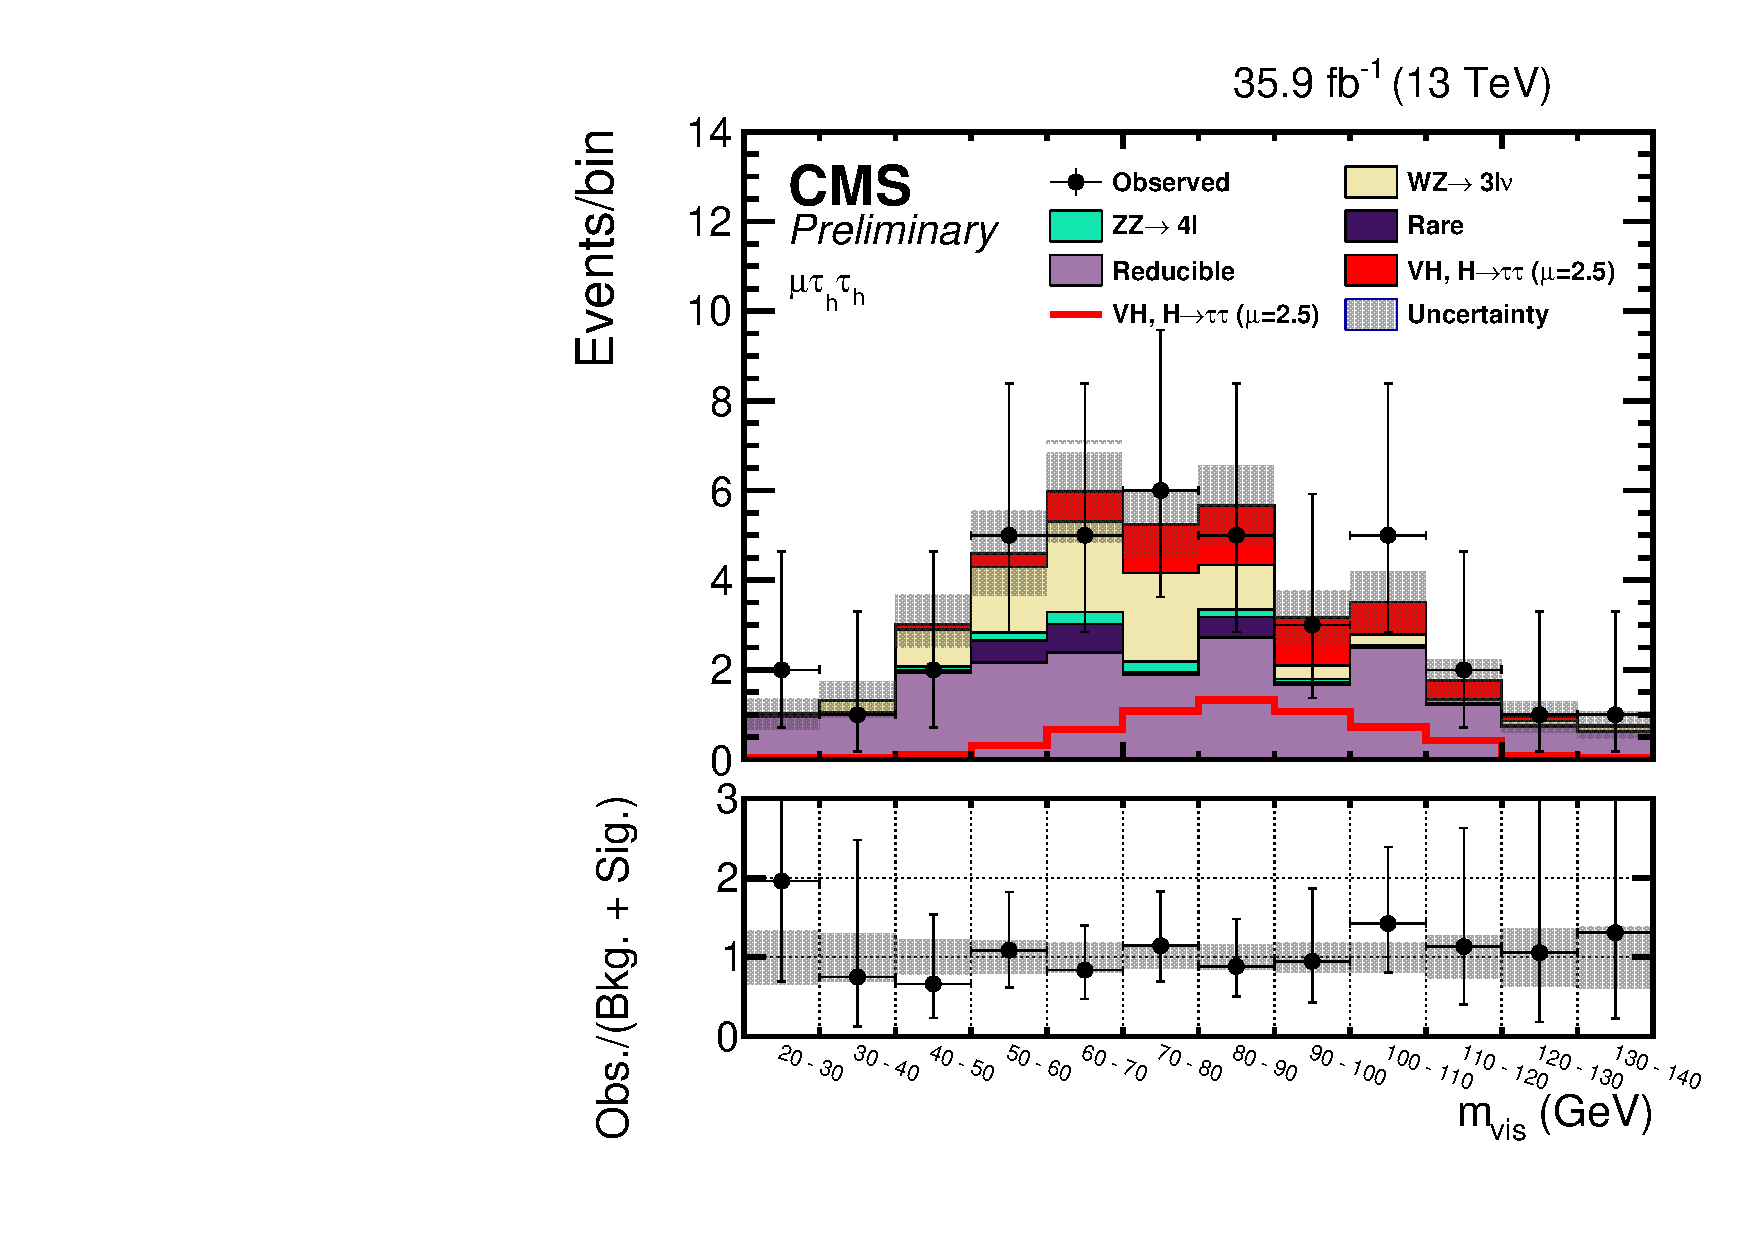
\includegraphics[width=0.49\textwidth]{higgs_to_taus_vh/plots/wh/mtt_postfit.pdf}
 \end{center}
 \caption{Postfit mass distributions in the $\Pe\Pgm\tauh$ (top left),
 $\Pgm\Pgm\tauh$ (top right), $\Pe\tauh\tauh$ (bottom left), and
 $\Pgm\tauh\tauh$ (bottom right) final states.
 The distributions show full uncertainties.
 The $\PW\PH$ and $\PZ\PH$, $\htt$ signal processes are summed together and 
 shown as $\VH$, $\htt$ with a best-fit $\mu = 2.5$. $\VH$, $\htt$ is shown both as 
 a stacked filled histogram and an open overlaid histogram. In these distributions 
 the $\PW\PH$, $\htt$ process contributes between 91\%--93\% of the total of $\VH$, $\htt$.
 }
 \label{fig:mass_whs}
\end{figure}

\begin{figure}[h!]
 \begin{center}
  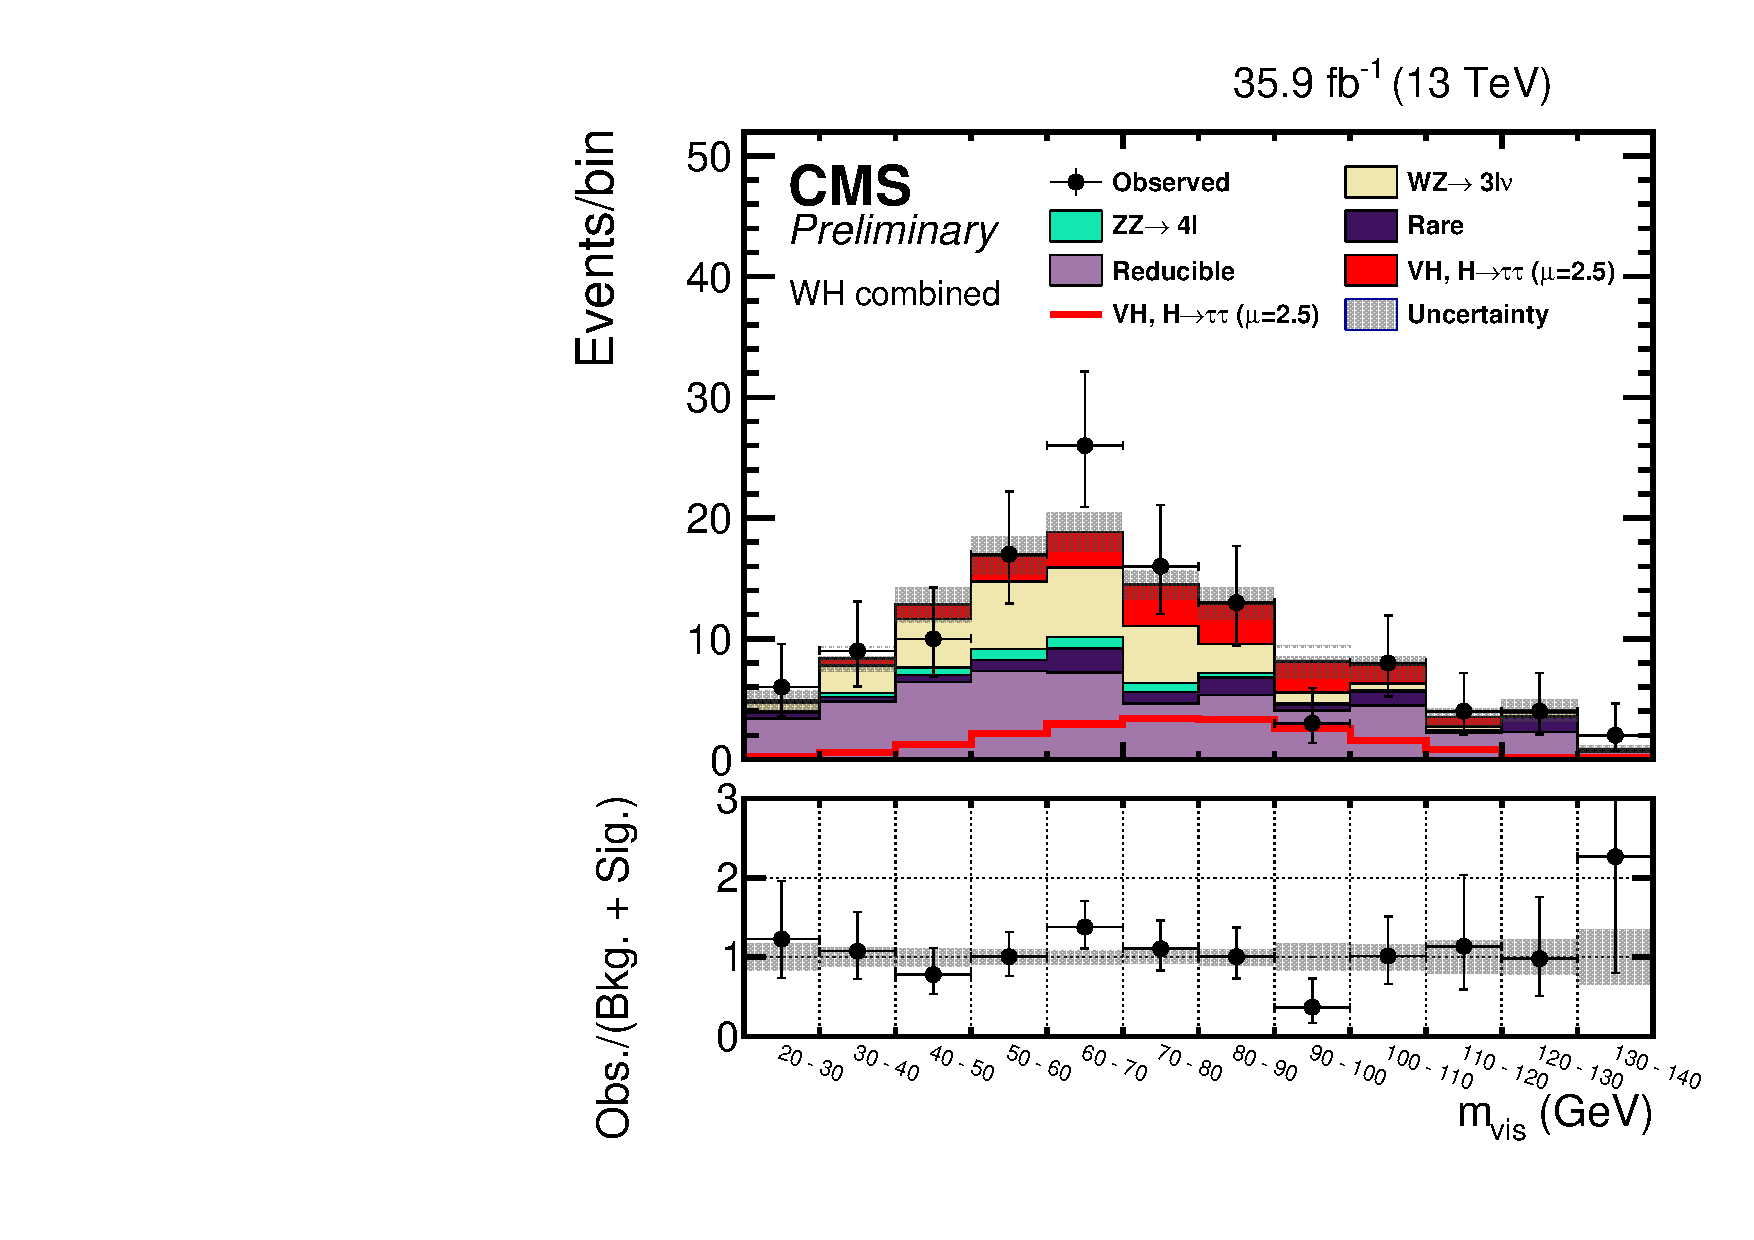
\includegraphics[width=0.65\textwidth]{higgs_to_taus_vh/plots/wh/wh_postfit.pdf}
 \end{center}
 \caption{Postfit mass distributions of the four $\PW\PH$ final states
 combined together. 
 The distributions show full uncertainties.
 The $\PW\PH$ and $\PZ\PH$, $\htt$ signal processes are summed together and 
 shown as $\VH$, $\htt$ with a best-fit $\mu = 2.5$. $\VH$, $\htt$ is shown both as 
 a stacked filled histogram and an open overlaid histogram. In this distribution 
 the $\PW\PH$, $\htt$ process contributes 92\% of the total of $\VH$, $\htt$.
 }
 \label{fig:mass_wh}
\end{figure}


\subsection{Analysis Sensitivity Details}
An excess of observed events with respect to the SM background expectation is 
visible in the most sensitive bins of the analysis, Figure~\ref{fig:sb}.
This distribution is created by grouping events in the signal regions 
by their decimal logarithm of the ratio of the 
signal ($S$) to signal-plus-background ($S+B$) in each bin

The postfit background and signal yields and the observed yields for the
$\PW\PH$ final states are shown in Table~\ref{tab:sb_wh} while those
for the $\PZ\PH$ final states are shown in Table~\ref{tab:sb_zh}. 
The $\PZ\PH$ final states are grouped according to the Higgs boson decay.

\begin{figure}[!ht]
 \begin{center}
  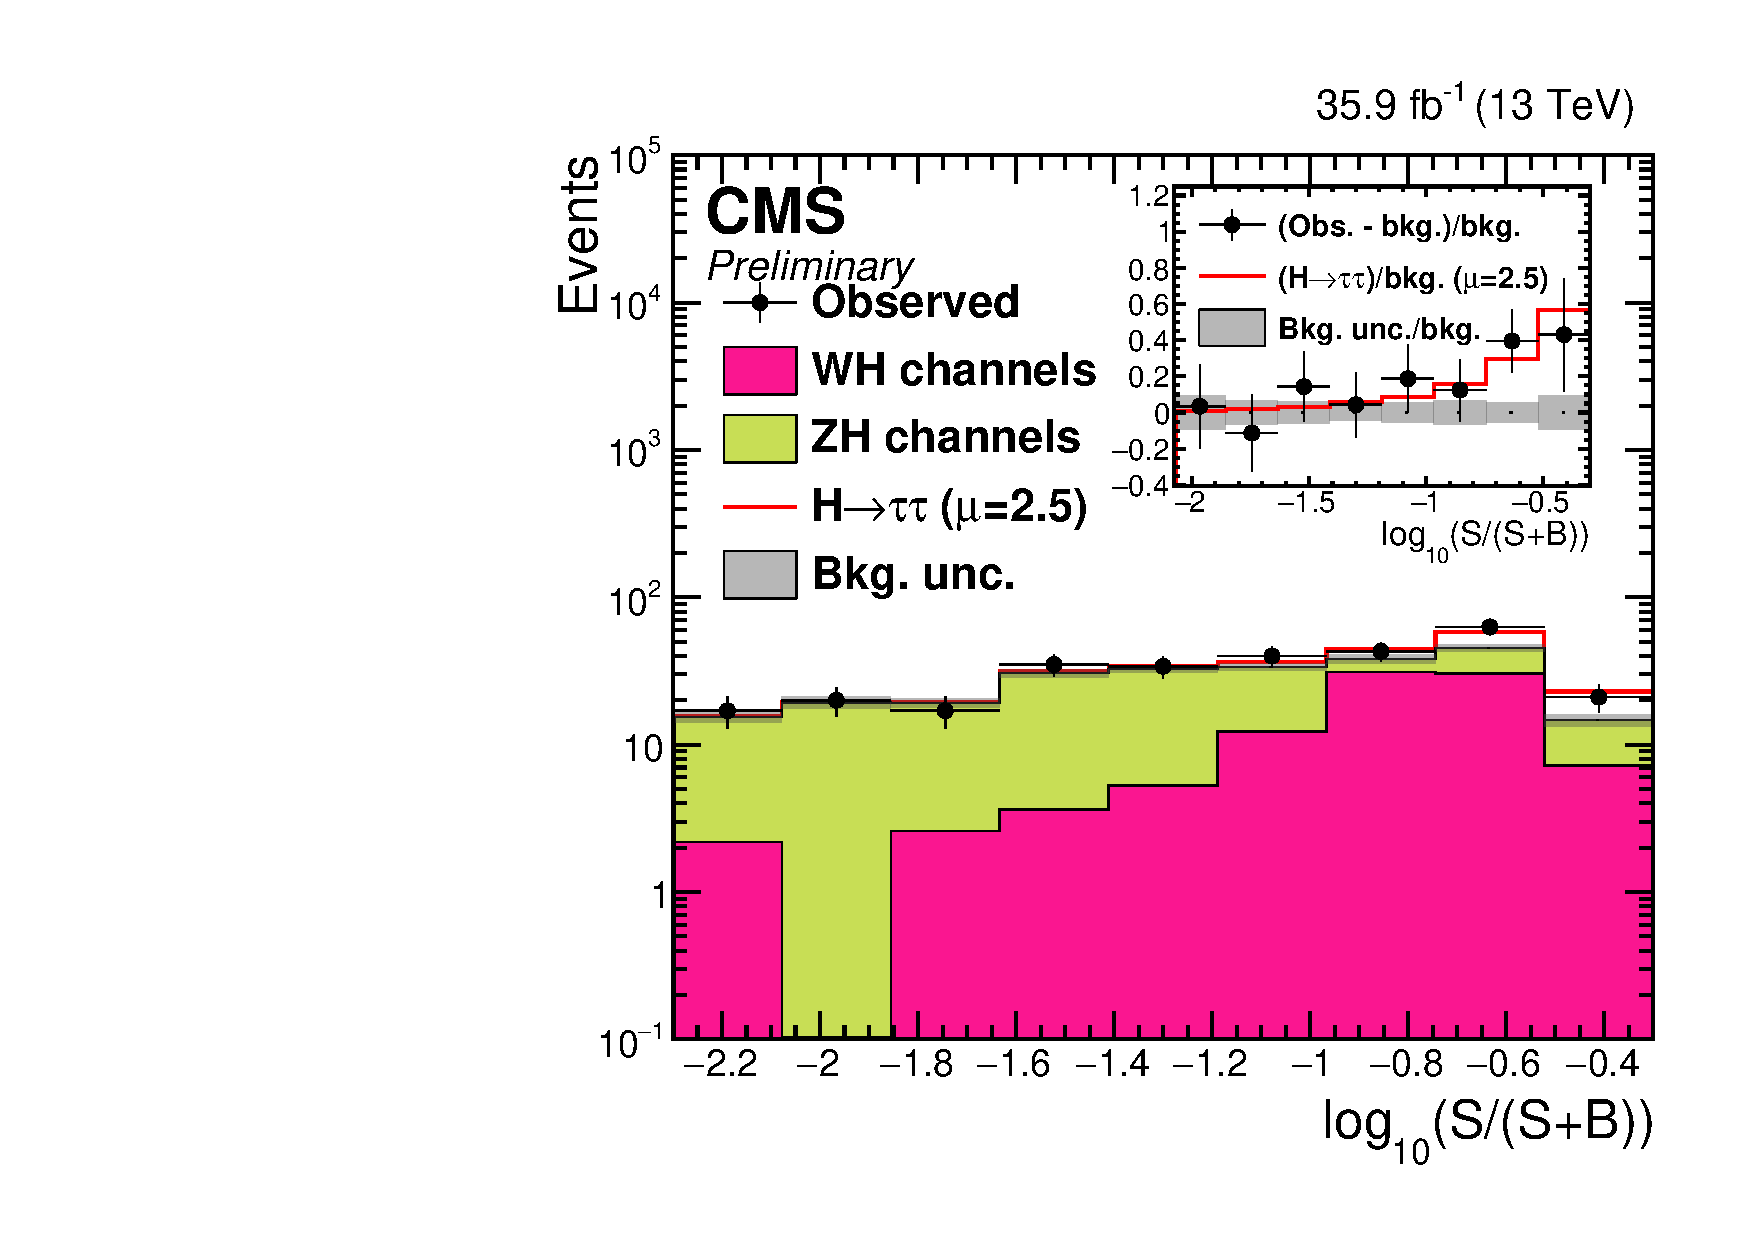
\includegraphics[width=0.55\textwidth]{higgs_to_taus_vh/plots/combined/wh_vs_zh_sbweight.pdf}
 \end{center}
 \caption{
 Distribution of the decimal logarithm of the ratio between the expected signal, 
 corresponding to the best fit value $\mu=2.5$, and the 
 sum of expected signal and expected background in each bin of the mass distributions 
 used to extract the results, in all signal regions. The background contributions are 
 separated based on the final states, $\PW\PH$ versus $\PZ\PH$. The inset 
 shows the corresponding difference between the 
 observed data and expected background distributions divided by the background expectation, 
 as well as the signal expectation divided by the background expectation.
 }
 \label{fig:sb}
\end{figure}

\begin{table*}
\centering
\begin{small}
\newcolumntype{x}{D{,}{\,\pm\,}{5.5}}
\begin{tabular}{lxxxx}
Process & \multicolumn{1}{c}{$\PW\PH, \Pe\Pgm\tauh$ } & \multicolumn{1}{c}{$\PW\PH, \Pgm\Pgm\tauh$ } & \multicolumn{1}{c}{$\PW\PH, \Pe\tauh\tauh$} & \multicolumn{1}{c}{$\PW\PH, \Pgm\tauh\tauh$}  \\
\hline
$\PZ\PZ$                  & 1.56, 0.05    & 0.93, 0.03  & 0.82, 0.04  & 1.18, 0.05   \\
$\PW\PZ$                  & 7.92, 0.28    & 6.69, 0.24  & 4.83, 0.25  & 8.38, 0.42   \\
Jet Fakes                 & 10.09, 1.61   & 12.19, 1.72 & 10.68, 1.27 & 19.80, 1.87  \\
Rare                      & 2.28, 0.61    & 3.77, 0.84  & 1.71, 1.08  & 1.76, 0.90   \\
Total backgrounds         & 21.85, 1.75   & 23.58, 1.92 & 18.04, 1.67 & 31.12, 2.12  \\
\hline
$\PW\PH, \PH \to\Pgt\Pgt$ & 4.28, 0.72    & 4.25, 0.73  & 3.51, 0.62  &  5.45, 0.97  \\
$\PZ\PH, \PH \to\Pgt\Pgt$ & 0.42, 0.07    & 0.40, 0.08  & 0.33, 0.07  &  0.44, 0.10  \\
Total signal              & 4.70, 0.72    & 4.65, 0.73  & 3.84, 0.92  &  5.98, 0.98  \\
\hline
%Observed &  \multicolumn{1}{c}{28 $\pm$ 5.3} &  \multicolumn{1}{c}{29 $\pm$ 5.4} &  \multicolumn{1}{c}{23 $\pm$ 4.8} &  \multicolumn{1}{c}{38 $\pm$ 6.2}  \\
Observed &  \multicolumn{1}{c}{28} &  \multicolumn{1}{c}{29} &  \multicolumn{1}{c}{23} &  \multicolumn{1}{c}{38}  \\
\hline
\end{tabular}
\end{small}
\caption{Background and signal expectations for the $\PW\PH$ final states, 
together with the number of observed 
events, for the post-fit signal region distributions.
The background uncertainty accounts for all sources of background uncertainty, 
systematic as well as statistical, after the global fit. The contribution from 
``Rare'' includes events from triboson, $\ttbar\PW$, $\ttbar\PZ$, $\ttbar\PH$ production,
and other rare processes.
}
\label{tab:sb_wh}
\end{table*}


\begin{table*}
\centering
\begin{small}
\newcolumntype{x}{D{,}{\,\pm\,}{5.5}}
\begin{tabular}{lxxxx}
Process & \multicolumn{1}{c}{$\ell\ell\Pe\tauh$} &  \multicolumn{1}{c}{$\ell\ell\Pgm\tauh$} &  \multicolumn{1}{c}{$\ell\ell\tauh\tauh$} &  \multicolumn{1}{c}{$\ell\ell\Pe\Pgm$} \\
\hline
$\PZ\PZ$                        & 14.40, 0.36 & 26.91, 0.55 & 25.58, 1.05 & 9.33, 0.18 \\   
Jet Fakes                       & 14.01, 1.55 & 17.58, 1.17 & 58.05, 2.87 & 3.66, 4.60 \\
Rare                            & 0.62, 0.08  & 1.54, 0.61  & 0.81, 0.42  & 3.02, 0.23 \\
Total backgrounds               & 29.03, 1.59 & 46.03, 1.43 & 84.44, 3.08 & 16.01, 4.61\\             
\hline
$\PW\PH, \PH \to\Pgt\Pgt$       & 0.008, 0.002  & 0.01, 0.003  & 0.016, 0.005  & 0.002, 0.001 \\
$\PZ\PH, \PH \to\Pgt\Pgt$       & 2.83, 0.39  & 5.31, 1.30  & 5.29, 1.17  & 1.62, 0.20 \\
Total signal                    & 2.84, 0.39  & 5.32, 0.70  & 5.31, 1.17  & 1.62, 0.20 \\
\hline
%Observed &  \multicolumn{1}{c}{33 $\pm$ 5.75} &  \multicolumn{1}{c}{53 $\pm$ 7.28} &  \multicolumn{1}{c}{87 $\pm$ 9.33} &  \multicolumn{1}{c}{20 $\pm$ 4.47}  \\
Observed &  \multicolumn{1}{c}{33} &  \multicolumn{1}{c}{53} &  \multicolumn{1}{c}{87} &  \multicolumn{1}{c}{20}  \\
\hline
\end{tabular}
\end{small}
\caption{Background and signal expectations for the $\PZ\PH$ final states, 
together with the number of observed 
events, for the post-fit signal region distributions. The $\PZ\PH$ final states
are each grouped according to the Higgs boson decay products. 
$\ell\ell$ covers both $\PZ \to \Pgm\Pgm$ and $\PZ \to \Pe\Pe$ events.
The background uncertainty accounts for all sources of background uncertainty, 
systematic as well as statistical, after the global fit. The contribution from 
``Rare'' includes events from triboson, $\ttbar\PZ$, $\ttbar\PH$ production,
and other rare processes.
}
\label{tab:sb_zh}
\end{table*}



\clearpage
